\documentclass[uplatex, a4paper, 12pt, openany, oneside]{jsbook}

\usepackage[dvipdfmx]{graphicx}
\usepackage[dvipdfmx]{color}
\usepackage[dvipdfmx, bookmarks=true, setpagesize=false]{hyperref}
\usepackage{subcaption} 
\usepackage{pxjahyper}
\usepackage{thesis}
\usepackage{here}
\usepackage{url}

\thesis{修 士 論 文}
% \title{
%   \centering
%     % \scalebox{1.0}{視覚と行動のend-to-end学習により経路追従行動を}\\
%     % \scalebox{1.0}{をオンラインで模倣する手法の提案}\\
%     % \scalebox{1.0}{-経路選択機能の追加とシナリオに基づく}\\
%     % \scalebox{1.0}{目的地へのナビゲーション-}\\
%     視覚と行動の end-to-end 学習により経路追従行動をオンラインで模倣する手法の提案\\
% -経路選択機能の追加とシナリオに基づく目的地へのナビゲーション-\\
% A proposal for an online imitation method of path-tracking behavior by end-to-end learning of vision and action\\
% -Adding route selection function and scenario-based navigation to the destination-\\
% }
\title{
  \centering
    \scalebox{0.7}{視覚と行動のend-to-end学習により}\\
    \vspace{-1.0zh}
    \scalebox{0.7}{経路追従行動をオンラインで模倣する手法の提案}\\
    \scalebox{0.7}{-経路選択機能の追加とシナリオに基づく目的地へのナビゲーション-}\\
    % \vspace{-0.3zh}
    \scalebox{0.7}{A proposal for an online imitation method of}\\
    \vspace{-1.0zh}
    \scalebox{0.7}{path-tracking behavior by end-to-end learning of vision and action}\\
    \scalebox{0.7}{-Adding route selection function and scenario-based}\\
    \vspace{-1.0zh}
    \scalebox{0.7}{navigation to the destination-}\\
    \vspace{-10zh}
}
\setlength{\textwidth}{\fullwidth}
\setlength{\evensidemargin}{\oddsidemargin}
\vspace{-30.0zh}
\date{2024年 3月}
\vspace{-30.0zh}
\teacher{林原 靖男 教授}
\vspace{-30zh}
\organization{千葉工業大学 先進工学研究科 未来ロボティクス専攻}
\author{22S1031  春山健太}
\vspace{-15zh}

\renewcommand{\baselinestretch}{1.2}
\begin{document}

%% Front Matter
\frontmatter{}
%
\chapter{動的に経路を選択して移動する機能の追加}
\label{chap:path_select}

\section{概要}
本章では,岡田らの従来手法に対して,目標とする進行方向のデータ
を加えることで,動的に経路を選択して移動する機能の追加を試みる.これにより,視覚に基づくナビゲーション
において,分岐路で「直進」「左折」などの任意の経路への移動
が可能となることを目指す.
以後,この動的に経路を選択して移動する機能を「経路選択機能」と呼ぶ
% \section{手法}
入力に目標方向を足した話
% \section{シミュレータを用いた実験}
シミュレータを用いて
経路選択機能の実験したよ.
% \section{実験結果}
同一の分岐路で,
選択できた

\section{経路選択機能を追加したシステム}
経路選択機能の追加を目的として,
データセットと学習器の入力へ,目標とする進行方向のデータ(以後,目標方向と呼ぶ)を新たに追加した.
\figref{fig:haru_mech_sys}に経路選択機能を追加したシステムを示す.
なお,上記の追加した要素を除き,他の部分は岡田らの従来手法と同様である.
学習時は,カメラ画像とメトリックマップに基づくルールベースの制御器から出力される
目標方向を入力としてデータセットへ加える.
岡田らの従来手法では,データセットの収集法に関して,いくつかバリエーションがある.
本論文では,その中で,最も経路追従の成功率が高い,学習器の出力とルールベース制御器の出力を比較し,
差の絶対値が閾値(0.05rad/s)を超えた場合のみ訓練データへ加える方法\cite{okada2021}を用いる.
学習後は,\figref{fig:path_select_abs}に示すように学習器へ外部から目標方向を入力する.
ロボットは視覚に基づくナビゲーションにおいて,入力された目標方向に従った経路を選択して移動する.

% 場所のデータのみ選択して訓練データに加える.
% 学習器の出力を監視して, 経路追従できない場所のデータのみ選択してデータセッ
% トに追加する手法を用いる.
\begin{figure}[htbp]
    \centering
     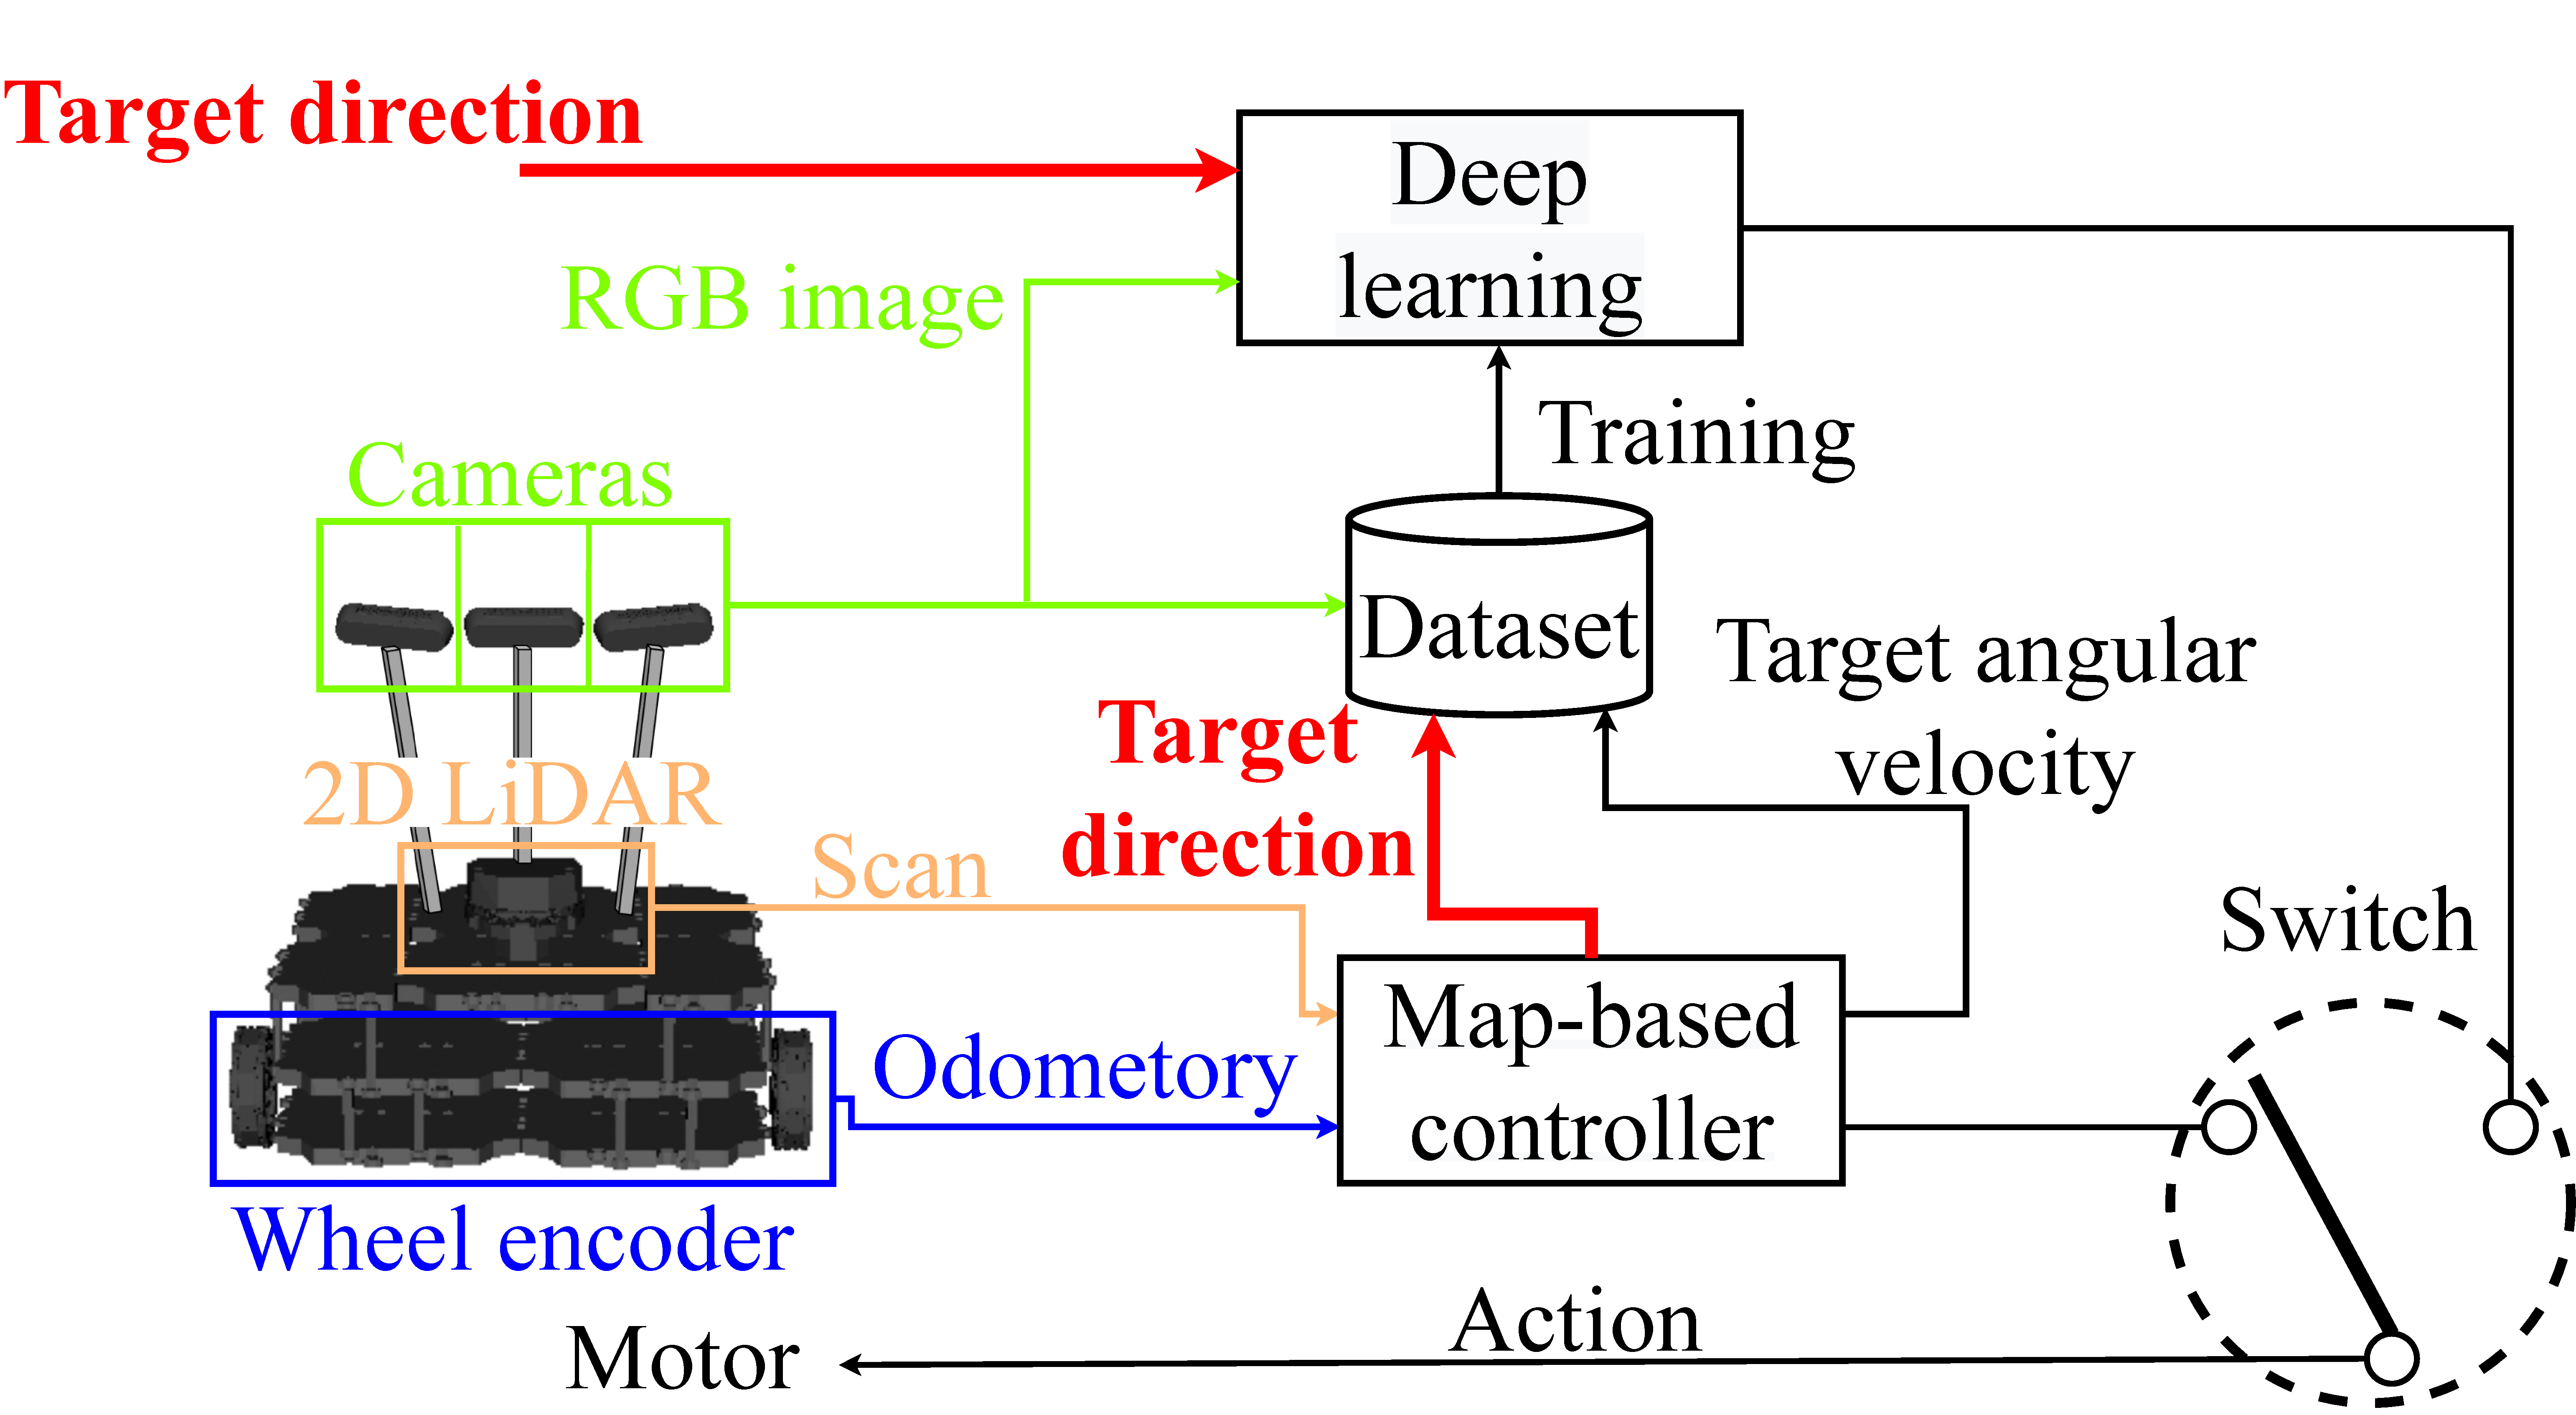
\includegraphics[width=130mm]{images/pdf/haru_mech_sys.pdf}
     \caption{System of the imitation learning with added function of
     selecting path}
     \label{fig:haru_mech_sys}
\end{figure}
\begin{figure}[htbp]
    \centering
     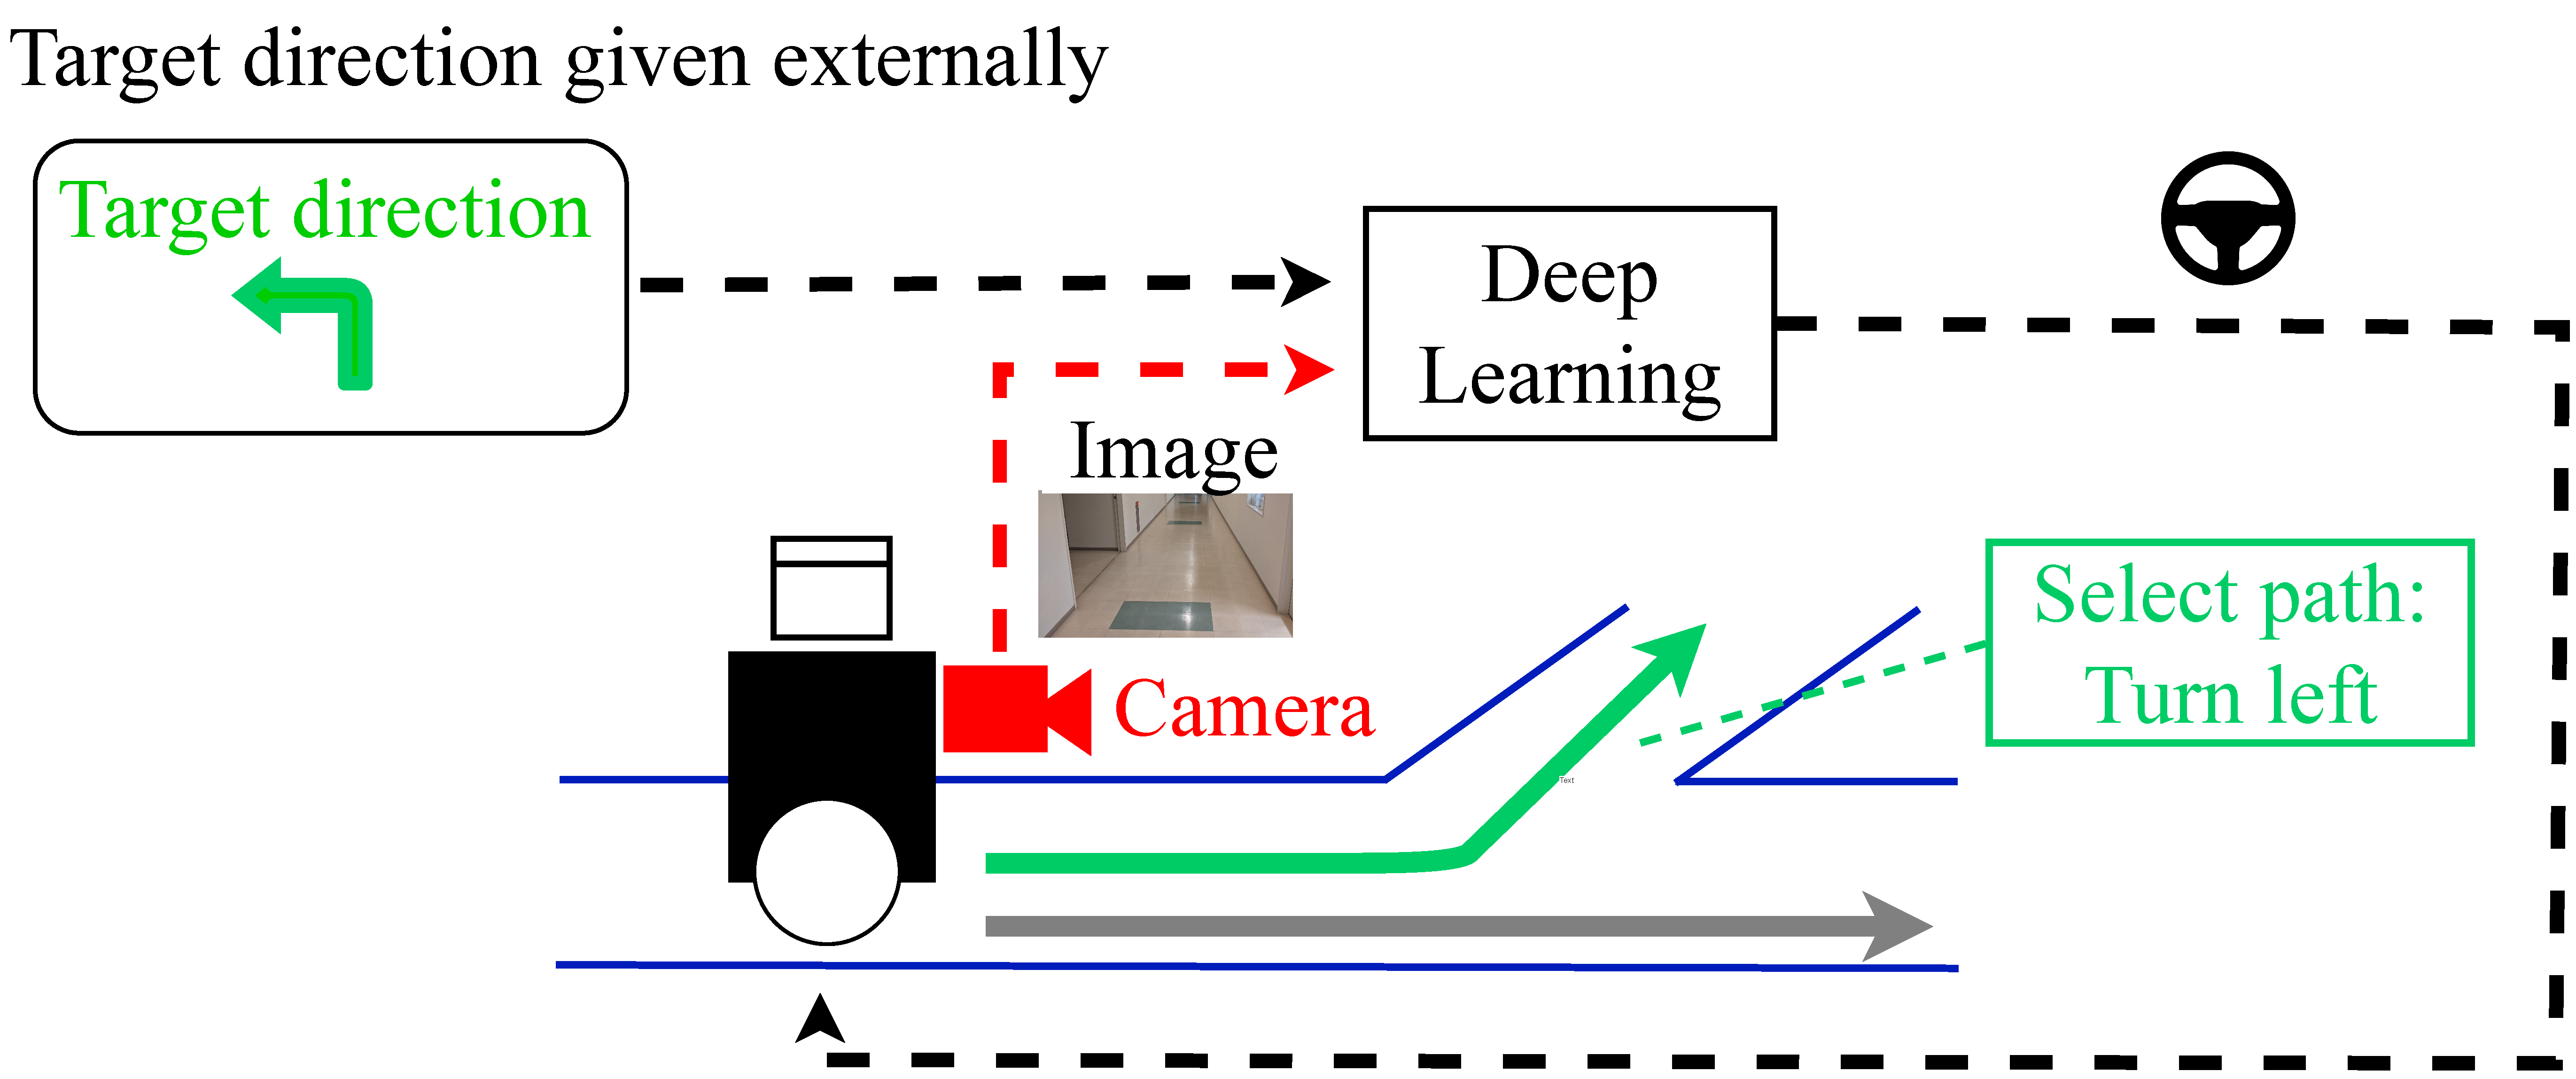
\includegraphics[width=130mm]{images/pdf/learning_gamma.pdf}
     \caption{Path selection and following behavior based on camera images 
     and target direction by imitation learning (Quoted from \cite{haruyama2023})}
     \label{fig:path_select_abs}
\end{figure}

\clearpage
\subsubsection{ネットワークの構造と目標方向のデータ形式}
経路選択機能を追加した学習器のネットワークの構造を\figref{fig:haru_mech_net}に示す.
岡田らの従来手法で用いたネットワークの出力部に,目標方向の入力部を追加した.
この層に\tabref{tab:target_old}に示すワンホットベクトルの
データを入力する.
ネットワークは,画像を処理するCNNアーキテクチャ,
CNNの出力と目標方向を入力とする全結合層で構成されている.
損失関数や活性化関数などのパラメータは岡田らの従来手法と同様である.

学習器はRGB画像と,目標方向を入力,ヨー方向の角速度を出力として
end-to-endで学習する.
つまり,視覚を入力とした行動を.目標方向によって条件付けながら学習する.
% 目標方向の
% 継続,直進,左折,右折の4つを
% ワンホットベクトルで表現する.
\begin{figure}[htbp]
    \centering
     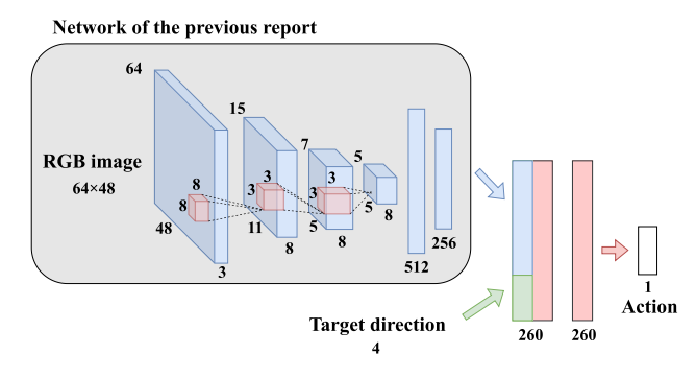
\includegraphics[width=130mm]{images/pdf/haru_mech.pdf}
     \caption{Structure of network with added function of
     selecting path}
     \label{fig:haru_mech_net}
\end{figure}

\begin{table}[htbp]
    \centering
    \caption{Target direction and data for imitation learning}\label{tab:target_old}
    \begin{tabular}{|c|c|}
    \hline
    Target direction & Data        \\
    \hline
    Continue   & {[}100,0,0,0{]} \\
    Go straight   & {[}0,100,0,0{]} \\
    Turn left   & {[}0,0,100,0{]} \\
    Turn right   & {[}0,0,0,100{]} \\
    \hline
    \end{tabular}
    \end{table}

\newpage
\section{シミュレータを用いた経路選択機能を確認する実験}
経路選択機能を追加したシステムで,指定した進行方向にロボットが移動できることを
シミュレータを用いた実験により確認する.
\subsubsection{実験装置}
実験はシミュレータ上で行い,シミュレータにはGazebo\cite{Gazebo}を使用し,
ロボットには\figref{fig:turtlebot3}に示すTurtleBot3 Waffle Pi\cite{ROBOTIS}へ3つのカメラを追加したモデルを用いる.
実験環境には,\figref{fig:haru_mech_exp}に示す千葉工業大学津田沼キャンパス2号館3階を模したモデルを用いた.
環境中のA,Bの地点においては,\figref{fig:haru_mech_exp_ab}に示すように侵入する方向が3つ,脱出する経路はそれぞれ2つ
あるため,バリエーションは6つある.
つまり,目標方向に従って適切に経路を選択して移動することが求められる場所となる
\begin{figure}[htbp]
    \centering
     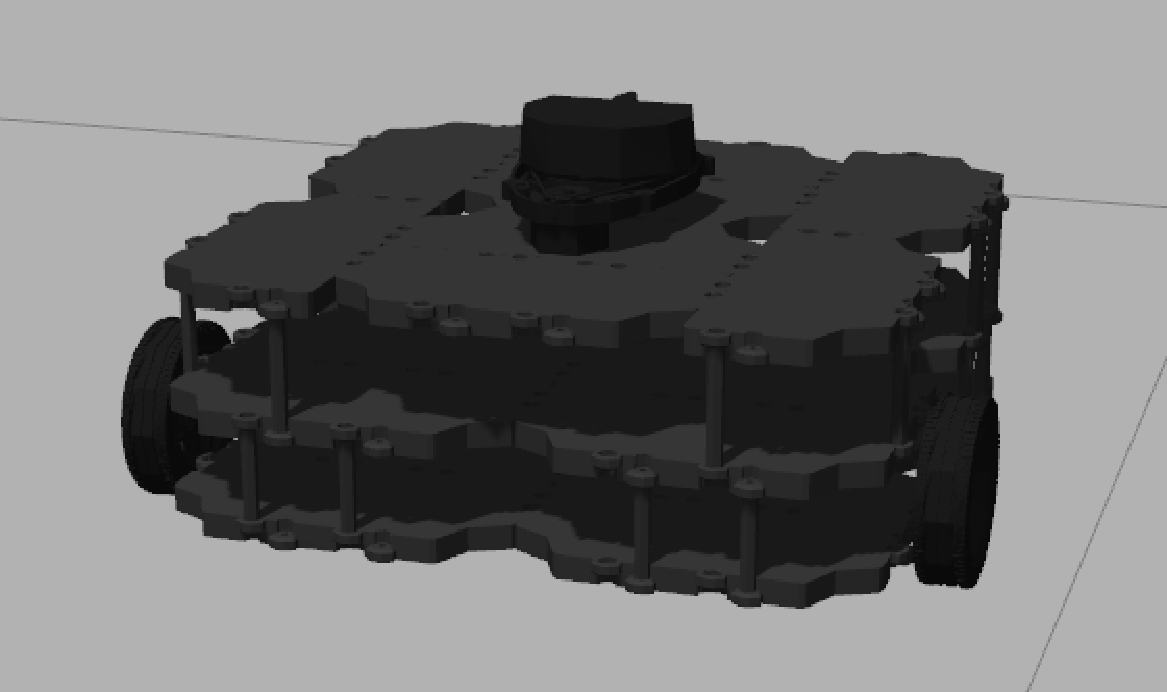
\includegraphics[width=80mm]{images/pdf/turtlebot3.pdf}
     \caption{TurtleBot3 Waffle Pi}
     \label{fig:turtlebot3}
\end{figure}
\begin{figure}[htbp]
    \centering
     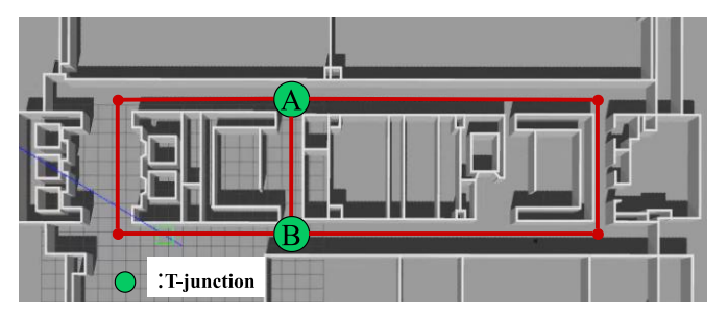
\includegraphics[width=130mm]{images/pdf/haru_mech_exp.pdf}
     \caption{Experimental environment of selecting path (Quoted from \cite{haruyama2022})}
     \label{fig:haru_mech_exp}
\end{figure}
\begin{figure}[htbp]
    \centering
     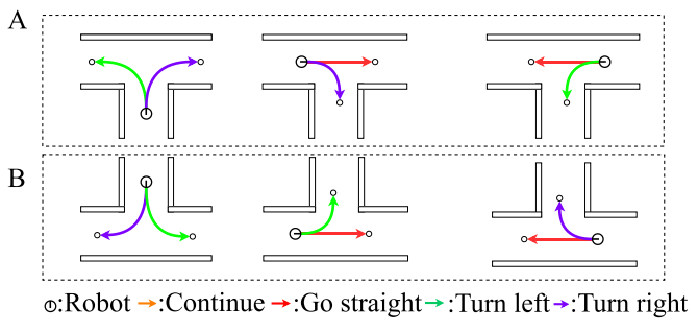
\includegraphics[width=130mm]{images/pdf/haru_mech_exp_ab.pdf}
     \caption{Selecting a path at the T-junction (Quoted from \cite{haruyama2022})}
     \label{fig:haru_mech_exp_ab}
\end{figure}
\vspace{-1zh}
\subsubsection{実験方法}
実験は,\figref{fig:haru_mech_route}に示した経路をaからfの順番で繰り返し走
行しながら,模倣学習を行う.目標方向のデータはメトリックマップに基づくルールベース制御器から出力
され,データセットに加えられる.学習は60000ステップ実行し,
その後視覚に基づくナビゲーションへ移行する.視覚に基づくナビゲーションにおいても
aからfまでの経路をロボットに走行させる.ロボットが壁に衝突した場合は,
ロボットを経路の中央まで戻して実験を継続する.
この実験を10回実施する.

\begin{figure}[htbp]
    \centering
     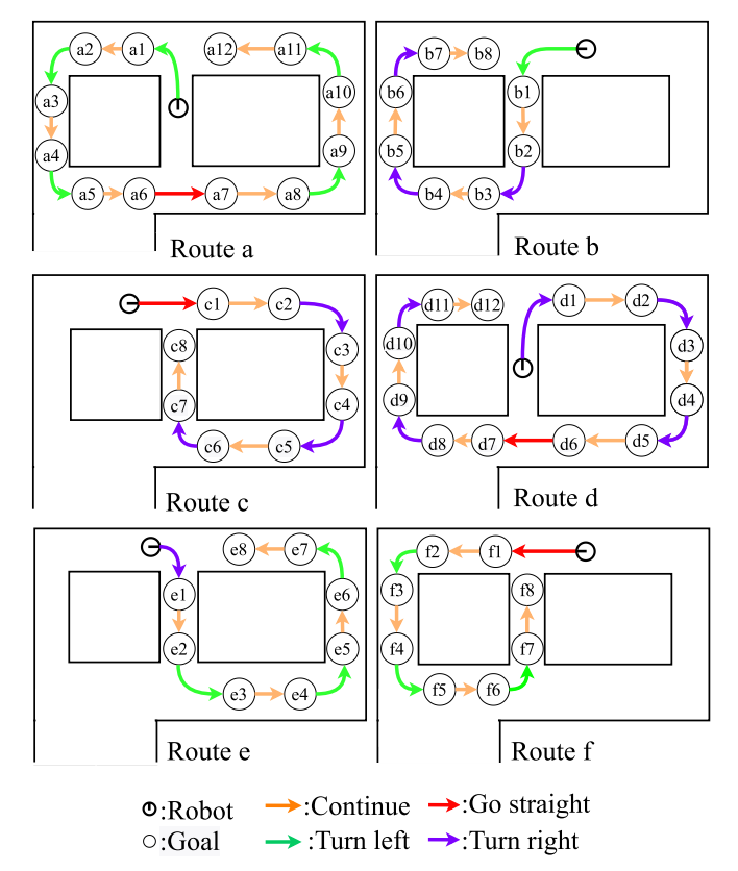
\includegraphics[width=130mm]{images/pdf/haru_mech_route.pdf}
     \caption{Route for experiment of selecting path (Quoted from \cite{haruyama2022})}
     \label{fig:haru_mech_route}
\end{figure}
\clearpage
\subsubsection{実験結果}
実験結果を\figref{fig:haru_mech_ab_res}に示す.
図はA,Bそれぞれの分岐路で,ロボットが正しく経路を選択した回数を示している.
図に示すように,目標方向に従い113/120回適切に経路を選択する様子が
確認できた.ただし,\tabref{tab:path_res}に示した箇所では,壁に衝突するな
どして自律移動が継続できない様子も見られた.

\figref{fig:haru_mech_a_select}にA地
点で目標方向のコマンドに従い,ロボットが経路を選択して
走行する様子を示す.このように,同一の分岐路であっても目
標方向の入力に従い,ロボットが適切に経路を選択して走行
する様子が見られた.
この結果から,岡田らの従来手法に対し,任意の目的地に向けた移動に必要な,動的に経路を選択した移動する機能を
追加できたと考えられる,
% \vspace{5zh}
\begin{figure}[htbp]
    \centering
     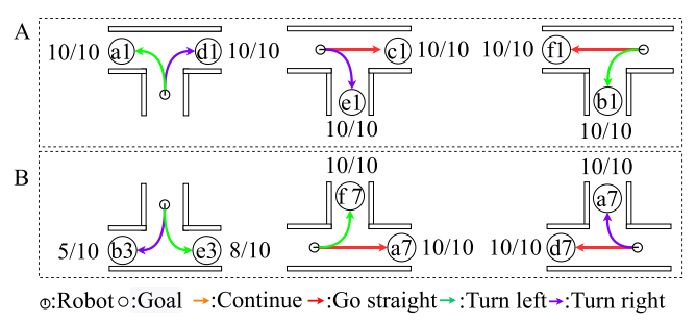
\includegraphics[width=130mm]{images/pdf/haru_mech_res.pdf}
     \caption{Number of times a correct path was selected (Quoted from \cite{haruyama2022})}
     \label{fig:haru_mech_ab_res}
\end{figure}
\vspace{-1zh}
\begin{table}[htbp]
    \centering
    \caption{Location where the robot went off course}\label{tab:path_res}
    \begin{tabular}{|c|c|c|}
    \hline
    Location & Number of Failed        \\
    \hline
    a5   & 2/10 \\
    b3   & 5/10 \\
    d11   & 1/10 \\
    e1  &  2/10 \\
    f5    & 2/10 \\
    \hline
    \end{tabular}
    \end{table}
\begin{figure}[htbp]
    \centering
    %  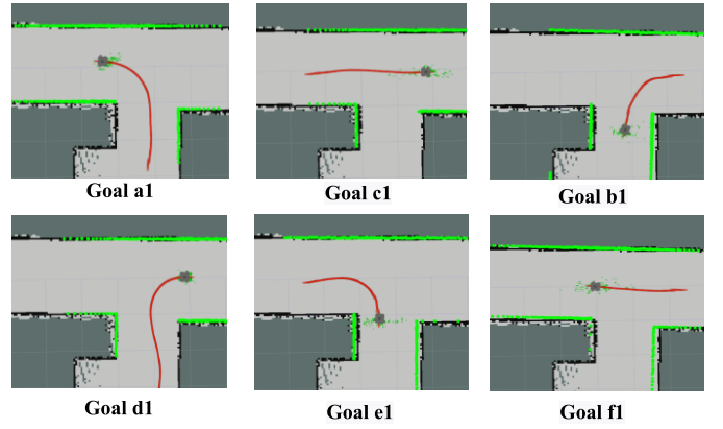
\includegraphics[width=120mm]{images/pdf/haru_mech_a_select.pdf}
     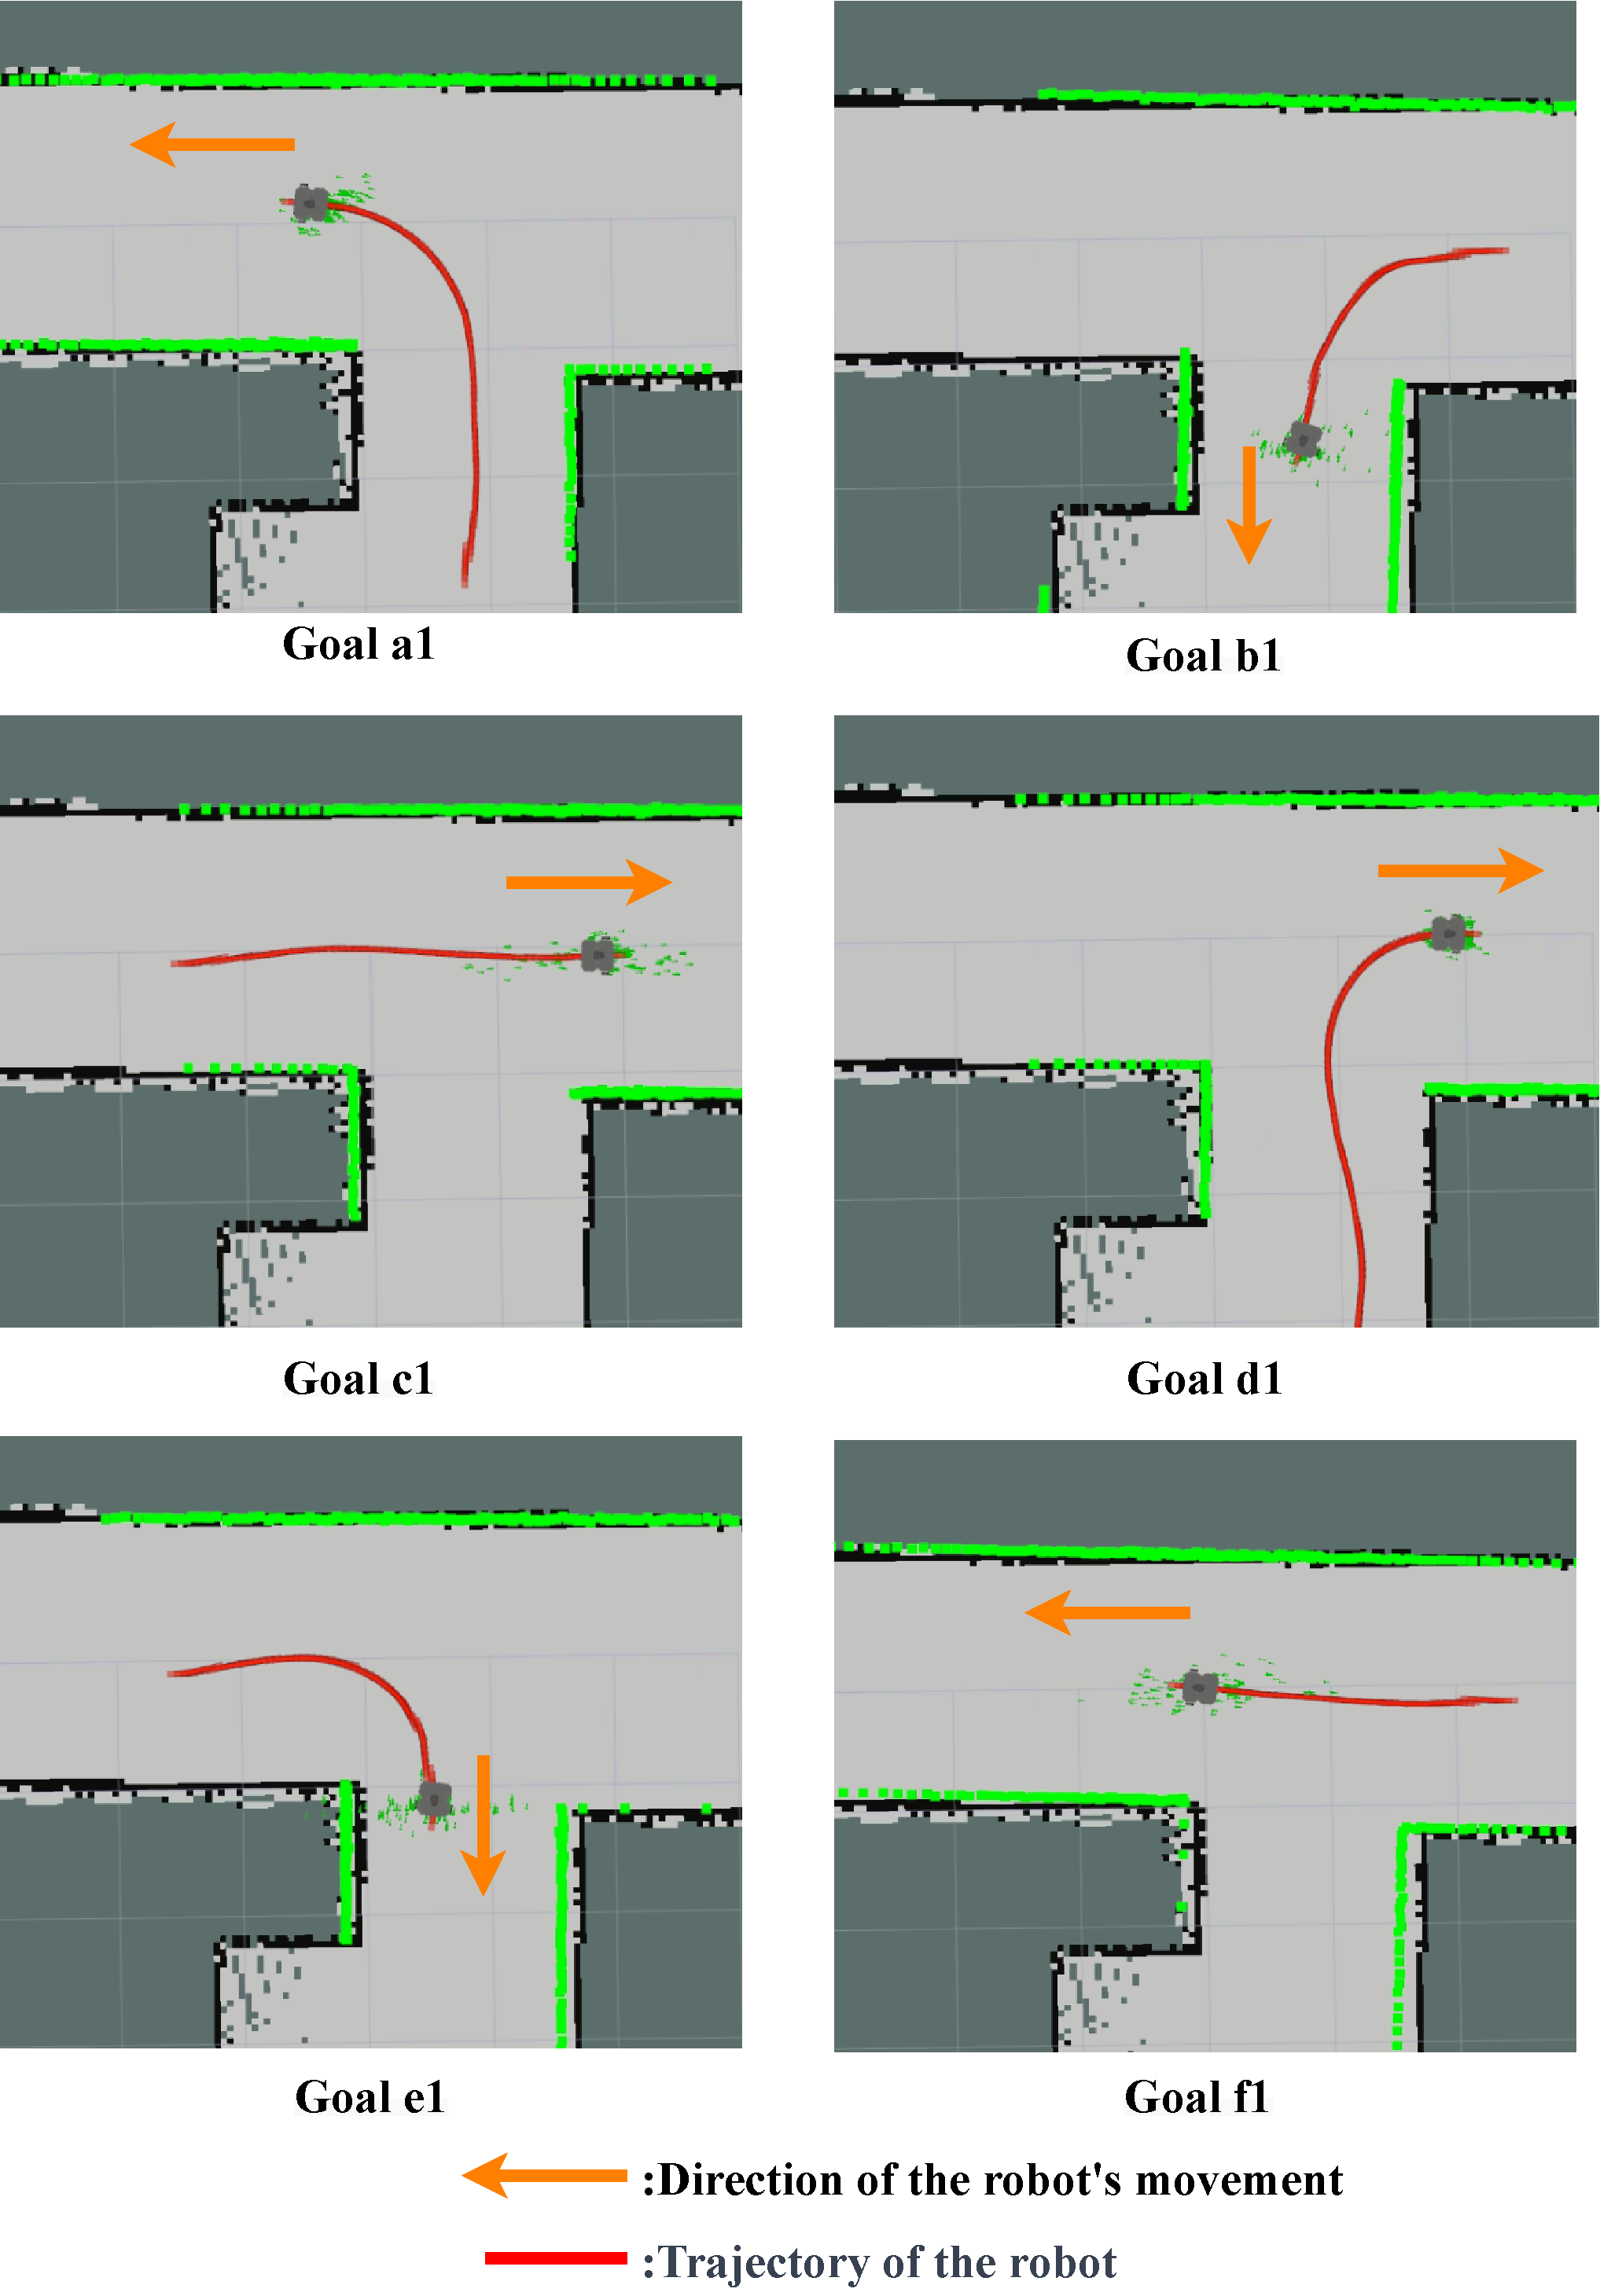
\includegraphics[width=130mm]{images/pdf/zyuziroute-select_a.pdf}
     \caption{The robot moving while selecting a path (Quoted from \cite{haruyama2022})}
     \label{fig:haru_mech_a_select}
\end{figure}

%
%% Main Matter
\mainmatter{}
%
\chapter{序論}
\label{chap:introduction}
%
%\input{introduction/preface}
%
%!TEX root = ../thesis.tex

\section{背景}
一般的に,移動ロボットを目的地まで誘導する制御はナビゲーションと呼ばれ,工場内の巡回や,警備.配送業務などを行う
自律移動ロボットに活用されている.
これらの多くのロボットは,ナビゲーションに
占有格子地図などの事前に作成したメトリックマップを用いている.
% に基づいて
% 自己位置推定,経路計画するナビゲーションにより目的地まで自律移動している.
例として,つくば市内の公道で行われる技術チャレンジである
つくばチャレンジにおいて,
原らが行なった技術調査\cite{hara2019}によると,参加した57チームの中で,50のチームが
メトリックマップに基づくナビゲーションを用いている.
また,これらのチームの多くは,メトリックマップに基づくナビゲーションに
LiDARやIMUなどのセンサ,ホイールエンコーダから算出したオドメトリを利用している.

これらのLiDARやオドメトリ,メトリックマップを基づくナビゲーション
の他に,カメラ画像と深層学習に基づくナビゲーションが研究\cite{kendall2018learning}\cite{sauer2018conditional}されている.
その中で,本研究室の岡田ら\cite{okada2020}\cite{okada2021}は\figref{fig:imi_abs}に示すように
メトリックマップを基づくナビゲーションによる行動を,
視覚を入力とした行動に模倣することで,視覚に基づくナビゲーションを
獲得する手法を提案した(以後,岡田らの従来手法と呼ぶ).
また,提案した手法の有効性を,シミュレータと実ロボットを用いて
検証する実験を行い,視覚に基づいて一定の経路を追従できることを確認している.
この手法の利点として,一般的な模倣学習が人の挙動を模倣するのに対して,
本手法では,メトリックマップに基づくナビゲーションの行動を模倣するため,データセットを収集する手間を省くことが可能という特長がある.
% 学習後はカメラ画像(視覚)のみをセンサ入力として自律移動が可能なことが挙げられる.
% また,メトリックマップに基づくナビゲーションと視覚に基づくナビゲーションを併用し,
% 状況に応じて高い信頼性が見込まれる方を選択することで,経路追従を継続できる可能性が高まる.

岡田らの従来手法では,経路を追従する行動の獲得を目的としていた.
そのため,走行する経路は一定という制限があり,任意の目的地に向けて移動することはできない.
\figref{fig:nav_need}に示す目的地に向けて移動するためには,
環境中の分岐路を検出する機能,分岐路で適切な進行方向を提示する機能,
動的に経路を選択して移動する機能が必要と考えられる.

そこで,本論文では,岡田らの従来手法に対し,
\figref{fig:haru_select}のような分岐路を視覚に基づいて検出する機能,
分岐路で目的地に向けた進行方向を提示する機能,
動的に経路を選択して移動する機能を追加する.
これにより,走行する経路を一定から,任意の目的地に向けた経路へ拡張することで,
視覚に基づいて,経路を追従して目的地へ到達できる可能性がある.
% 目的地までの経路の指示
% また,分岐路といった「通路の特徴」を検出する機能の
% 分岐路で経路が選択できること.
% 目的地までの経路の指示

% カメラ画像
% 実世界では,LiDARやGNSSなどのある特定のセンサが機能しない状況に
% おちいり.ロボットの自律移動を継続することが困難になる場合がある.
% この問題の対処には,複数のセンサを統合して利用する方法や,ロボットに
% ナビゲーション手段自体を複数持たせる(冗長化)する方法が考えられる.

% ナビゲーション手段の冗長化に向けて,
% 本研究室の岡田らは,\ref{fig:imi_abs}に示すように
% 一般的に用いられるLiDARやオドメトリ,
% メトリックマップに基づくナビゲーションの行動を
% 視覚を入力としてend-to-endで模倣学習することで,
% 視覚に基づくナビゲーションを獲得する手法を提案している.
% この手法の特長として,学習のデータセットに利用する行動と
% 学習時にロボットを制御する行動を別々にして扱うことで
% ロボットが経路から外れたときでも,常に経路に戻る行動をデータセットに追加できる.
% また実験を通して,視覚に基づいてロボットが学習した経路を周回可能であることが確認した.
% 岡田らはさらに,訓練時に計測したデータの全てをデータセットに加えるのではなく, 学習器の出力
% を監視して, 経路追従できない場所のデータのみ選択してデータセットに追加する手法を追加している.
% これにより,目標角速度のデータセットの偏りを減少し,角の経路でも経路を追従できる可能性が向上することが
% 確認されている.
\vspace{3zh}
\begin{figure}[htbp]
     \centering
      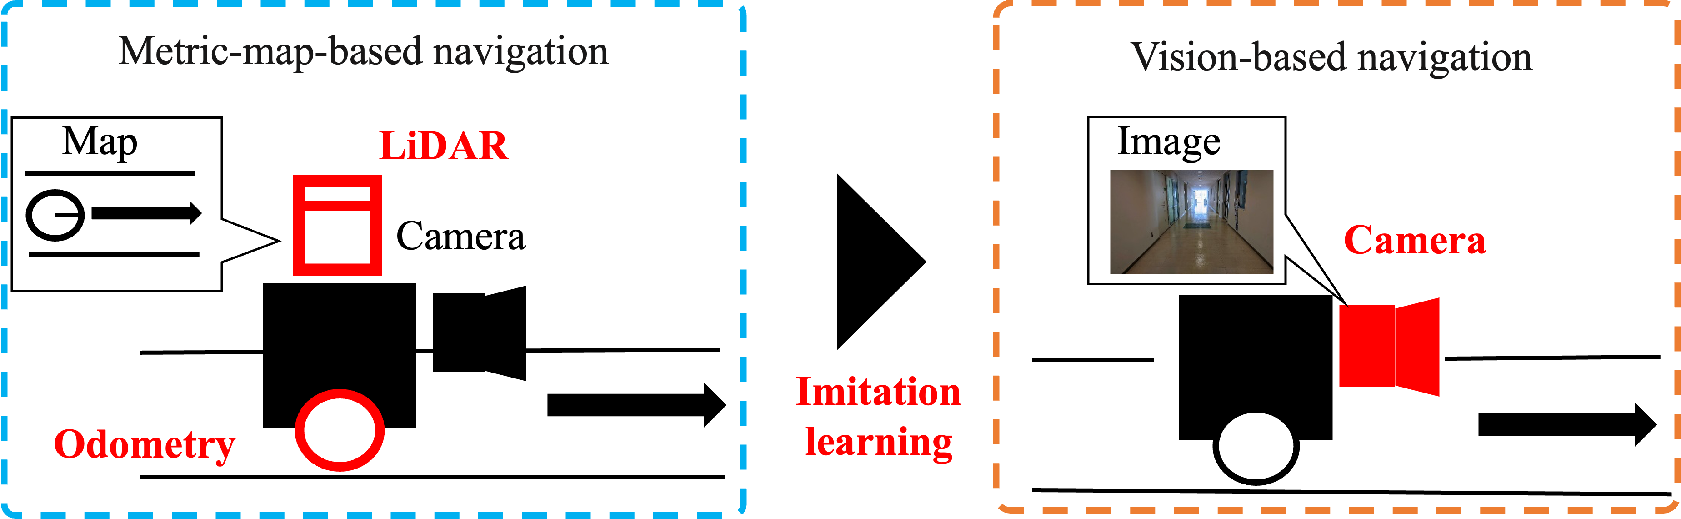
\includegraphics[width=130mm]{images/pdf/imi_abs.pdf}
      \caption{Imitation method of path-tracking behavior}\label{fig:imi_abs}
 \end{figure}


% 春山らは,前述の岡田らの手法に対し,
% 目標とする進行方向の情報(目標方向)を加えることで,
% 視覚に基づくナビゲーションに分岐路で経路を選択して移動する
% 機能を追加している.
% これにより,ロボットは\ref{fig:haru_select}のように
% 指示された方向に移動するように,
% カメラ画像に基づいて経路を移動する
% また,藤原らは,この経路を選択する機能を学習する際に,
% オーバーサンプリングや学習時に積極的に蛇行する手法を取り入れることで,
% 学習時間を短縮する手法を提案している.
% 岡田らの手法では,周回する経路を
\begin{figure}[htbp]
     \centering
      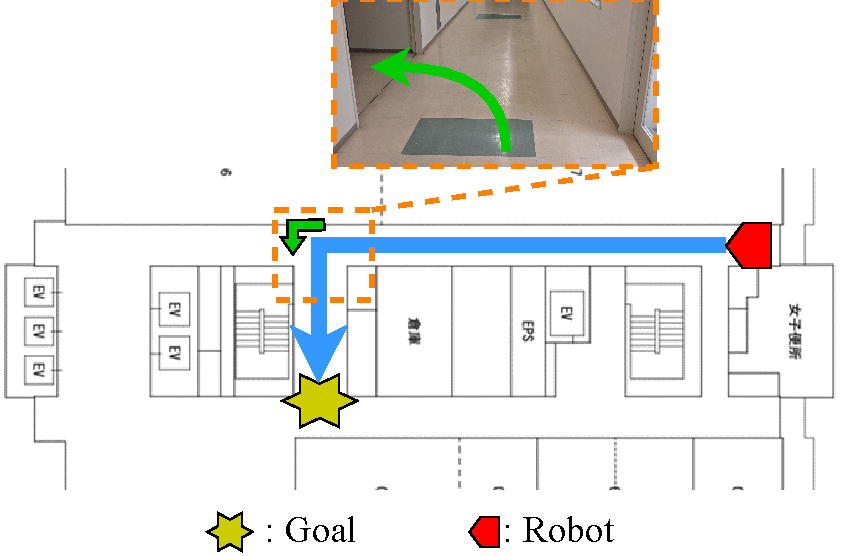
\includegraphics[width=90mm]{images/pdf/nav_need.pdf}
      \caption{Autonomous mobility towards any destination}\label{fig:nav_need}
 \end{figure}
 \begin{figure}[htbp]
     \centering
      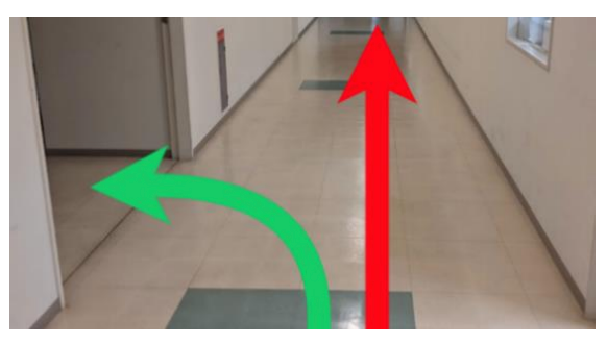
\includegraphics[width=90mm]{images/pdf/branch_path.pdf}
      \caption{Path selection and following behavior based 
      on camera images and target direction by imitation learning}\label{fig:haru_select}
 \end{figure}
% 春山らと藤原らの手法では,目標方向の
% 作成方法は議論の対象としておらず,
% 分岐路における目標方向の生成は,カメラ画像から行っていない.
% つまり,視覚のみで目的まで自律移動することは困難となっていた.
% そこで,本稿では,視覚のみで目的地まで自律移動するために,
% 前述の経路を選択する機能をもつ視覚に基づくナビゲーションに対し,
% 目的の分岐路に到達したかの判定を視覚で行い,目標方向を提示する機能を追加
% を追加する.
% このシステムにより,事前に作成したメトリックマップを必要せずに,
% カメラ画像を入力として目的地まで自律移動できる可能性がある.
\newpage

%
% \section{要素技術}
本章では,本研究に関連する要素技術を述べる
\subsection{深層学習}
\subsection{教師あり学習}
\subsection{end-to-end学習}
\subsection{Convolutional Neural Network (CNN)}
\subsection{Long Short Term Memory(LSTM)}
\subsection{メトリックマップに基づくナビゲーション}
ナビゲーションは
本稿では,事前にLiDARやオドメトリなどのセンサを使用して作成したした占有格子地図を用いた目的地までの
自律移動手法をメトリックマッベースの自律移動と呼ぶ.
ROS Navifation stackを用いている.
自己位置推定
自己位置推定ではパーティクルフィルタによって自己位置推定を行うモンテカルロ自己位置推定(MCL)
経路計画
経路計画では占有格子地図からコストマップ ダイクストラ法やA*による
速度指令
本稿では,模倣学習やデータセットの作成に使用している.
\subsection{トポロジカルマップ}
トポロジカルマップは,環境中のランドマークなどの特徴的な箇所(ノード)とその繋がり(エッジ)によって
環境を表現したマップである.
トポロジカルマップをロボットのナビゲーションに適応した研究は〜や〜がある.
本稿でのトポロジカルマップは前述の島田らが提案した形式のものを指す

\subsection{シナリオ}
シナリオはトポロジカルマップ上での,目的地までの経路を
単語の組み合わせで表現したものである,
シナリオは条件と行動で構成される
このシナリオの形式は,人の道案内に関する情報のアンケートによって得られた情報に基づき決定された.


\newpage
\clearpage
\section{関連研究}
分岐路で動的に経路を選択して移動する機能を有する視覚に基づくナビゲーションを,模倣学習により
獲得する手法はいくつか提案されている.
Felipeら\cite{codevilla2018endtoend}は視覚を入力とする模倣学習を,
左折や右折などの行動ごとにモデルを分けて行った.
このモデルを目標とする経路方向のベクトルによって切り替えることで,\figref{fig:felipe}に示す
経路選択が可能な視覚に基づく自律移動を行なっている.
\begin{figure}[htbp]
    \centering
     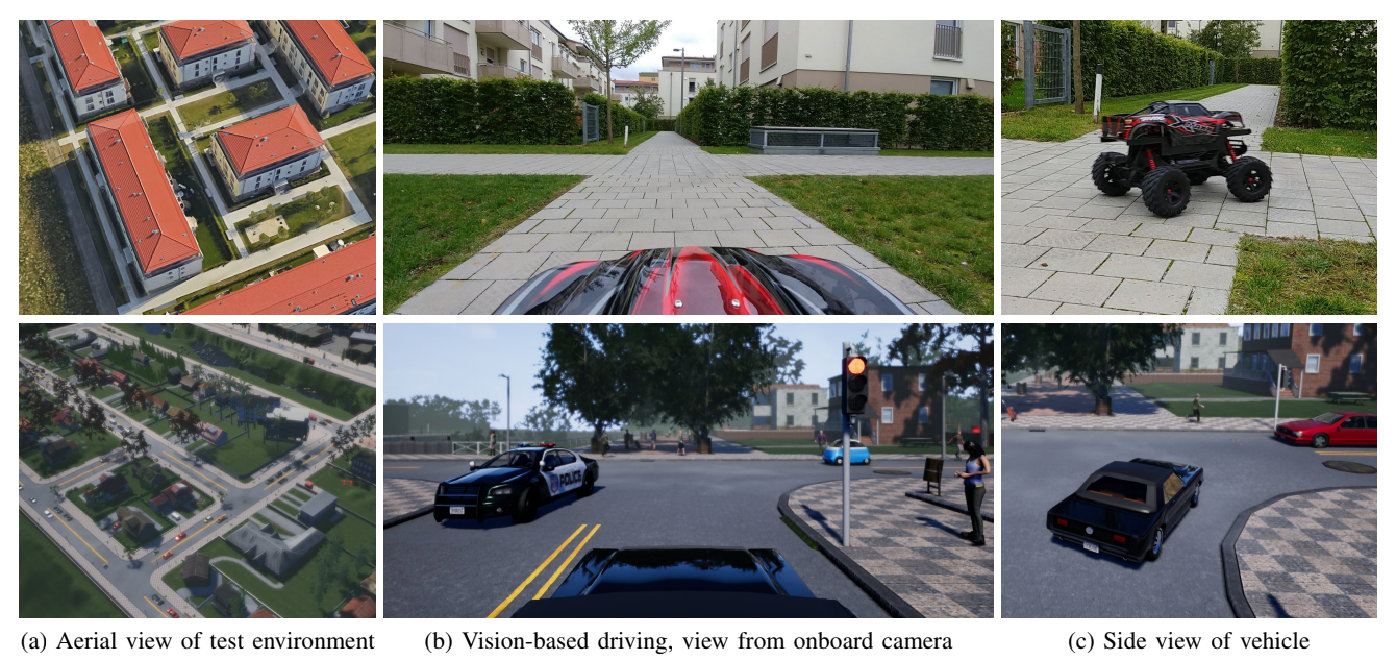
\includegraphics[width=120mm]{images/pdf/fleipe.pdf}
     \caption[End-to-end driving via conditional imitation learning]{End-to-end driving via conditional imitation learning(Quoted from\cite{codevilla2018endtoend}}
     \label{fig:felipe}
\end{figure}

Seiyaら\cite{seiya2018}は\figref{fig:seiya}に示すようにカメラ画像と目的地への方向を示すベクトルを入力,
ステアリングの角度を出力として模倣学習を行なった.
これにより視覚に基づくナビゲーションにおいて,屋内外の分岐路で目的地への方向を示すベクトルを与えることで,
特定の経路が選択できることを確認している.
\begin{figure}[htbp]
    \centering
     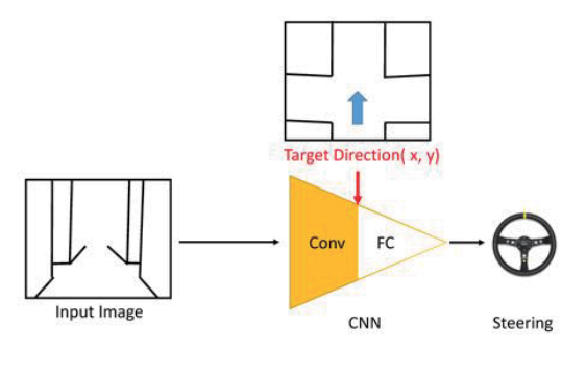
\includegraphics[width=100mm]{images/pdf/seiya.pdf}
     \caption[Overview of Seiya and others proposed method]{Overview of Seiya and others proposed method(Quoted from\cite{seiya2018}}
     \label{fig:seiya}
\end{figure}

これらの研究により,経路の情報を含めて模倣学習することで,経路選択が可能な
自律移動を獲得できることが確認されている.
\chapref{chap:path_select}ではこれらの
研究を参考に,岡田らの従来手法に対し,経路を選択する機能の追加を試みる.
\newpage
次に
任意の目的地に向けて移動が可能な視覚に基づくナビゲーションに
関連した研究について述べる.
Dhruvら\cite{shah2022lmnav}は,
大規模な事前学習モデルを用いて,自然言語指示と画像を組み合わせたナビゲーションを提案している.
この研究では,\figref{fig:lmnav}に示すように,
自然言語で指示されたランドマークを視覚によって検出し,これらのランドマークを経由して目的地へ自律移動する.
% 目的地までランドマークを辿ることでナビゲーションを行う.
実験では,停車中の車,道路標識,曲がり角といった道路の特徴をランドマークとして利用している.

\begin{figure}[htbp]
    \centering
     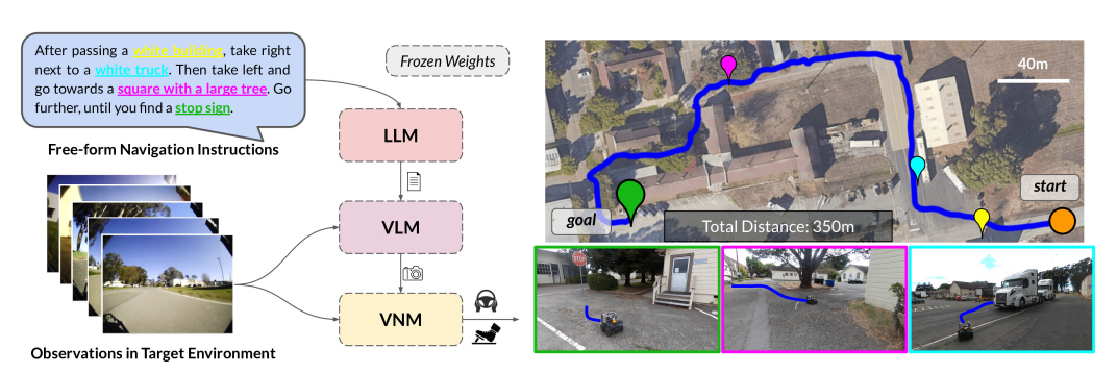
\includegraphics[width=120mm]{images/pdf/lmnav.pdf}
     \caption[Embodied instruction following with LM-Nav]{Embodied instruction following with LM-Nav(Quoted from\cite{shah2022lmnav}}
     \label{fig:lmnav}
\end{figure}
\newpage
Miyamotoら\cite{miyamoto}は環境中のランドマークを含む\figref{fig:topo_meiji}に示すトポロジカルマップと,
\figref{fig:seg_meiji}に示すセマンティックセグメンテーションを用いた,視覚に基づくナビゲーションを提案している.
実験では,木などの植物や,建物,交差点などのランドマークを視覚によって検出し,
これらをトポロジカルマップ上での経路の決定に利用している.


\begin{figure}[h]
    \centering
     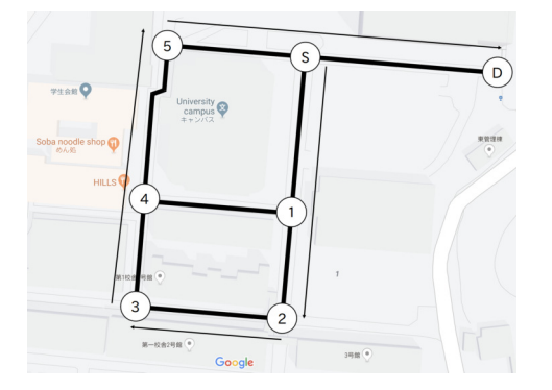
\includegraphics[height=60mm]{images/pdf/topo_meiji.pdf}
     \caption[Miyamoto and others used topological map]{Miyamoto and others used topological map(Quoted from\cite{miyamoto})}
     \label{fig:topo_meiji}
\end{figure}
\begin{figure}[h]
    \centering
     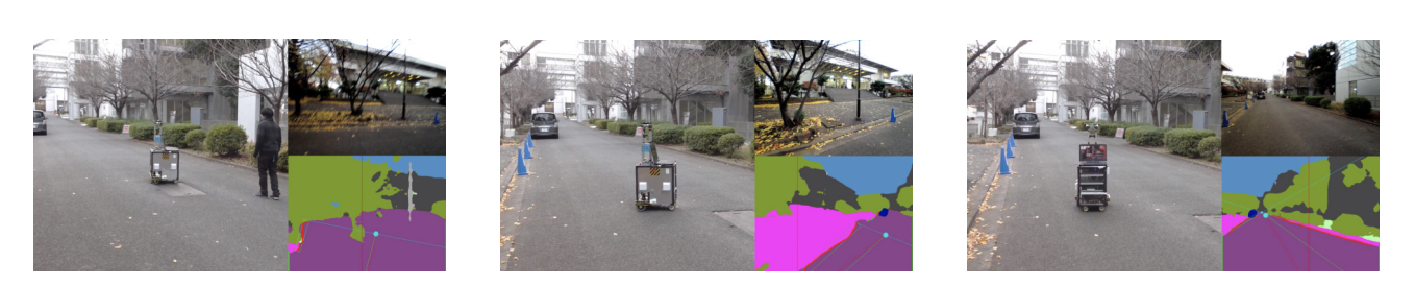
\includegraphics[width=120mm]{images/pdf/seg_meiji.pdf}
     \caption[Observation of robot behavior using semantic segmentation]{Observation of robot behavior using semantic segmentation(Quoted from\cite{miyamoto})}
     \label{fig:seg_meiji}
\end{figure}

% これらの研究から,視覚に基づくナビゲーションにおいて,
% 設定した目的地まで自律移動するためには,標識や交差点といったランドマークの検出が
% 必要な要素であることが明らかになっている.
% 本論文では,分岐路において動的に経路を選択して移動することから
% 「分岐路」などの通路の特徴をランドマークとして扱い,これを視覚に基づいて検出する.

これらの研究では,視覚に基づくナビゲーションにおいて,目的地への自律移動に
標識や交差点といったランドマークを用いている.
本論文では,分岐路で動的な経路を選択した移動を行うことから,「分岐路」などの通路の特徴を
ランドマークとして扱い,これを視覚に基づいて検出する.

% 手法では,補助的ではあるが,Global Navigation Satellite System(GNSS)や
% ホイールオドメトリといった情報を必要としている.
% センサ入力という観点で比較すると,\chapref{chap:scenario_vision}で述べるシステムは
% カメラ画像のみで目的地まで移動できるという違いがある.
\newpage
\section{目的}
本論文では,カメラ画像のみで目的地に移動するために,
視覚に基づくナビゲーションに対して,
視覚から分岐路の判別,目標方向を提示する機能を追加する.
これにより,カメラ画像とトポロジカルマップから
作成されるシナリオに基づいて,目的地まで自律移動するシステムを構築,提案する.
また,提案するシステムにより
目的地までカメラ入力のみで自律移動できるかを,
実ロボットを用いた実験により検証する.

\section{論文構成}
\ref{chap:introduction}章では本論文における,背景や関連研究,目的を述べた.
\ref{chap:elemental}章では本論文に関連する要素技術を述べる,
\ref{chap:method}章では本論文で提案するシステムについてのべ,
\ref{chap:experiment}章では提案するシステムの有効性を
実ロボットを用いて検証する実験に関して述べる.
\ref{chap:end}章では,本論文の結論と展望を述べる.
%ここにディレクトリのパスを追加していく
\chapter{要素技術}
\label{chap:elemental}
本章では,本研究に関連する要素技術を述べる
\section{深層学習}
\subsection{教師あり学習}
教師あり学習は,機械学習の一種であり,
データセットと呼ばれる
ラベル付きのデータの集合を使用してモデルを訓練する手法である.
データセットには,入力データとそれに対応する正解(ラベル)が含まれている.
モデルはデータセットを利用して,正解となる出力を得られるように学習を行っていく.

\subsection{end-to-end学習}
\ref{fig:e2e}に示すように,入力されるデータから目的の出力を得るために必要なデータを得るために必要な
他段階の処理をニューラルネットワークを用いて直接学習する手法である.
自律移動を例に述べる.
人物や障害物などの物体認識,走行レーンの検出,
経路計画,ステアリング制御などの複数個のタスクを解く必要があるが, 
end-to-end学習では先程のタスクを人間が直接設定せずに
カメラ画像をニューラルネットワークに入力することで,
直接ステアリング操作を学習する.
\begin{figure}[htbp]
    \centering
     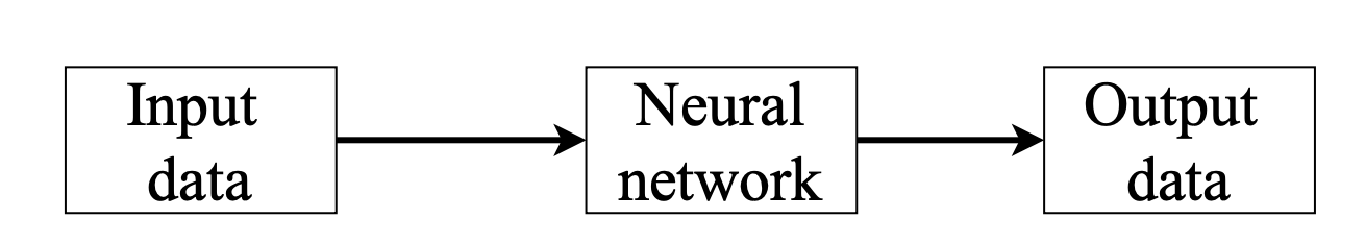
\includegraphics[width=90mm]{images/pdf/e2e.pdf}
     \caption{Structure of end-to-end learning}
     \label{fig:e2e}
\end{figure}

\newpage
\section{メトリックマップに基づくナビゲーション}
一般的に,移動ロボットを目的地まで誘導する制御はナビゲーションと呼ばれている.
その中で,事前にLiDARやオドメトリなどのセンサを使用して作成した占有格子地図などの
地図を用いたナビゲーション手法がある.
本稿ではこの地図に基づくナビゲーションを
「メトリックマップに基づくナビゲーション」と呼ぶ.
このメトリックマップに基づくナビゲーションを提供するルールベース制御器として
ROS Navigation stack\cite{ros}がある.
\begin{quote}
    \begin{itemize}
     \item パーティクルフィルタによって自己位置推定を行うモンテカルロ自己位置推定(MCL)
     \item 障害物認識などの局所的または地図全体の大域的なコスト計算と,その結果に基づく経路計画
     \item 経路に追従する並進速度や角速度などの速度指令
    \end{itemize}
   \end{quote}
この中で,経路を追従する行動を「経路追従行動」と呼ぶ.
本論文では,Navigation stackをこの模倣学習やデータセットの作成に使用している.
% \vspace{5zh}
\begin{figure}[htbp]
    \centering
     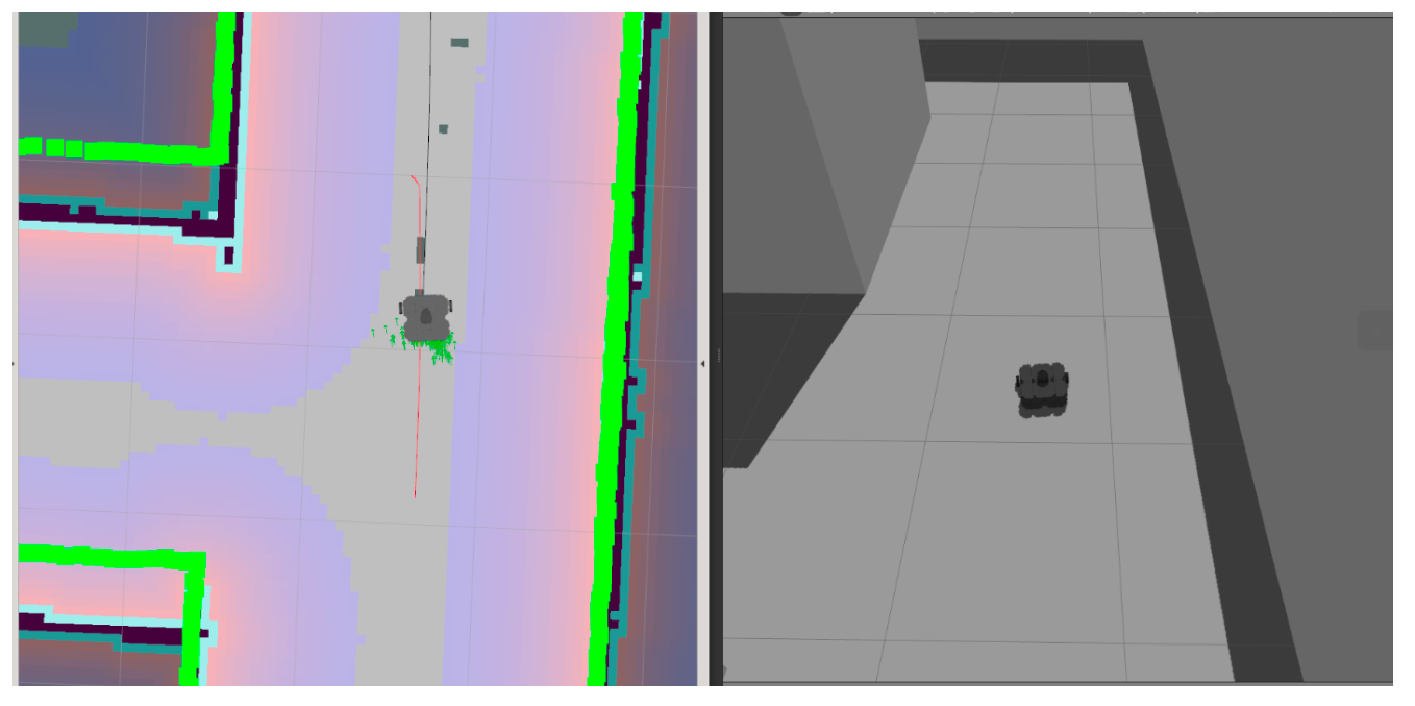
\includegraphics[width=100mm]{images/pdf/nav.pdf}
     \caption{Path-following module system Quoted from\cite{shimada2020}}
     \label{fig:nav}
\end{figure}

\newpage
\section{トポロジカルマップ}
トポロジカルマップは,環境中のランドマークなどの
特徴的な箇所(ノード)とその繋がり(エッジ)によって
環境を表現したマップである.
島田らは\ref{fig:topo}に示すようなトポロジカルマップの形式\cite{shimada2020}を提案している
トポロジカルマップのノードは,
人の道案内に関するアンケートにおいて,
通路の特徴が多用されていたため,該当する位置に配置され,
その位置がどのような通路の特徴であるかという情報を
持っている.また,「直進」や「右折」といった~で述べるシナリオの行動から
移動するエッジを選択するために,ノードはエッジのIDと相対角度の情報を
持っている.エッジはノードの接続関係を表すように
ノード同士を結んでいる.多くの研究では距離に関する情報を持っていることが
多いが,島田らの形式ではIDのみを持っている.
本稿で用いるトポロジカルマップは,島田らが提案した形式を指す.
\begin{figure}[htbp]
    \centering
     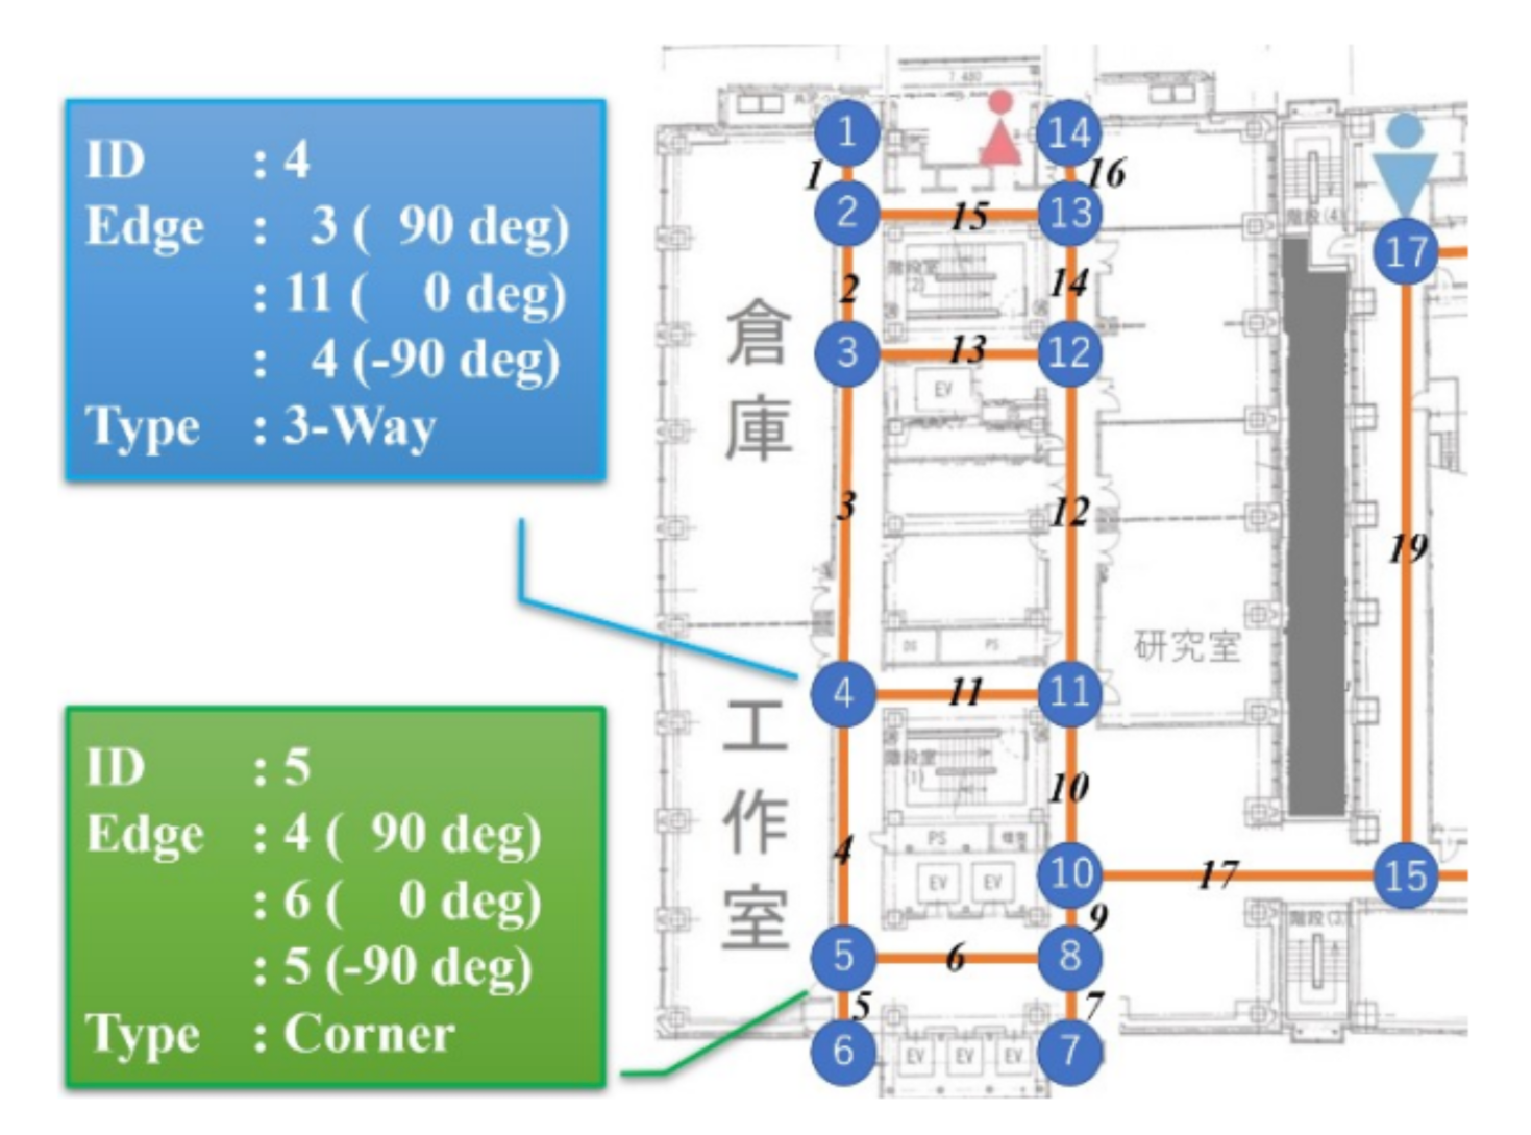
\includegraphics[width=90mm]{images/pdf/topo.pdf}
     \caption{Path-following module system Quoted from\cite{shimada2020}}
     \label{fig:topo}
\end{figure}
\newpage
\section{シナリオ}
シナリオはトポロジカルマップ上での,目的地までの経路を単語の組み合わせで表現したものである,
シナリオは「次の角」や「突き当たり」のような「条件」と「直進」,「右折」のような「行動」の組み合わせにより作成される.
このシナリオの形式は,トポロジカルマップと同様に
人の道案内に関するアンケートで得た,
「次の角まで」のような「条件」と「左折」などの「行動」を組み合わせているという
情報を基に決定している,
例えば,\ref{fig:scenario01}に示すような経路をシナリオで表すと,「3番目の三叉路まで直進.停止」となる,
\begin{figure}[htbp]
    \centering
     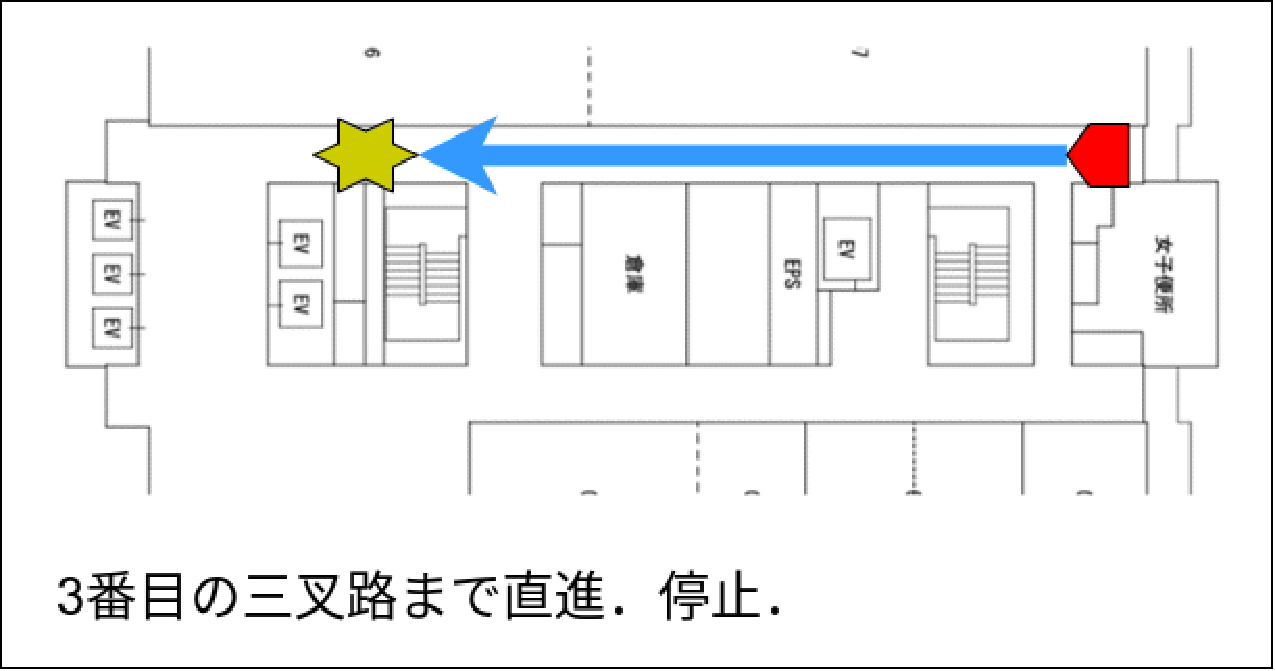
\includegraphics[width=90mm]{images/pdf/scenario/scenario01.pdf}
     \caption{Path-following module system Quoted from\cite{shimada2020}}
     \label{fig:scenario01}
\end{figure}
\chapter{先行研究}
本論文の議論のベースとなる,岡田らの従来手法と
島田らが提案したトポロジカルマップの形式,単語の組み合わせで経路を表現したシナリオについて述べる

\section{視覚と行動のend-to-end学習により経路追従行動を
オンラインで模倣する手法}
岡田らの従来手法について述べる.
岡田らの従来手法では,メトリックマップに基づくナビゲーションの経路追従行動をend-to-end学習により,
視覚を入力とした行動へ模倣する.
これにより,視覚に基づくナビゲーションを獲得できる.
手法に基づいて構築されたシステムを\figref{fig:okada_sys}に示す.

まずはじめに,学習器の訓練を行う.
学習器の訓練時,LiDARやオドメトリを入力とするメトリックマップに基づく
ルールベース制御器を用いて,設定した経路を追従する.
その際,ロボットに取り付けた,カメラから得たRGB画像とルールベース制御器が出力する
ヨー方向の角速度をペアとして0.2秒の周期でデータセットへ加える.
次にデータセットから,バッチサイズを8として教師データを抽出し,0.2秒の周期で
end-to-end学習する.
このデータセットへのデータの追加から学習までの1連の流れを1ステップとしている.
カメラ画像の収集には,3つのカメラを用いる.
左右のカメラ画像に対するヨー方向の角速度は,経路に戻るようなオフセット(\(\pm 0.2\)rad/s)を加える.

学習器の訓練後は,学習器へ中央のカメラから得たRGB画像を入力し,出力されるヨー方向の角速度を用いて経路を追従する.
この時,並進速度は0.2m/sの一定の値を用いる.
\vspace{10zh}
\begin{figure}[htbp]
    \centering
     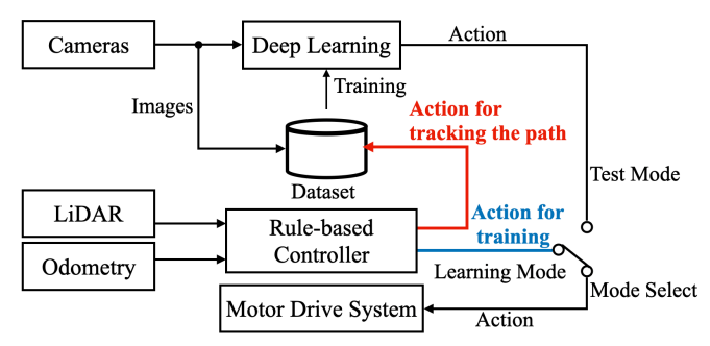
\includegraphics[width=110mm]{images/pdf/okada_method_sys.pdf}
     \caption{Structure of the Okada and others proposed system (Quoted from\cite{okada2020})}
     \label{fig:okada_sys}
\end{figure}
\clearpage
この岡田らの従来手法は,ルールベース制御器を教師データの収集に用いることで,
データセットの収集に人間の操作が不要となること,
\figref{fig:robo_ac}に示すように学習のデータセットに加える行動と
学習時にロボットを制御する行動を別々に
扱うことで,常に経路に戻る行動のみをデータセットに追加できるといった特長がある.
\begin{figure}[htbp]
    \centering
     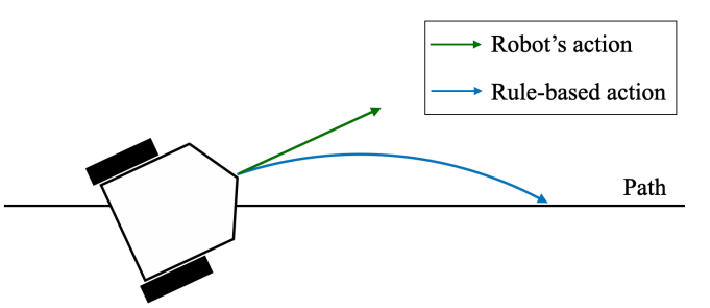
\includegraphics[width=100mm]{images/pdf/robo_action.pdf}
     \caption{Rule-based actions
     apart from the robot's actions Quoted from\cite{okada2020}}
     \label{fig:robo_ac}
\end{figure}

\figref{fig:okada_net}
に岡田らの従来手法における学習器のネットワーク構造を示す.
ネットワークは,入力層 1,畳み込み層 3,全結合層 2,出力層 1 の全7層で構成される.
活性化関数としてReLU\cite{relu},最適化アルゴリズムにAdam\cite{adam},
損失関数としてはSoftmax-cross-entropyを用いる.
学習器は入力を64x48のRGB画像データ,出力をロボットのヨー方向の角速度として
end-to-end学習する.
\begin{figure}[htbp]
    \centering
     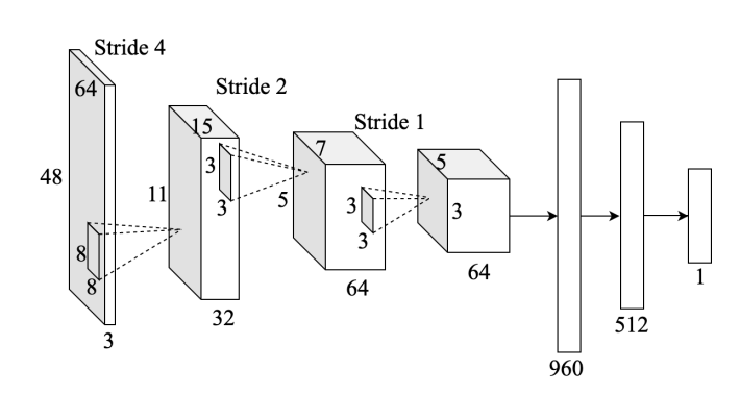
\includegraphics[width=100mm]{images/pdf/okada_network.pdf}
     \caption{Structure of the network used in the method of Okada and others. (Quoted from \cite{okada2020})}
     \label{fig:okada_net}
\end{figure}

\clearpage
\section{トポロジカルマップとシナリオ}
\label{sec:shimada_topo}
ここでは,分岐路で適切な進行方向を提示する機能のベースとなる,
島田ら\cite{shimada2020}が提案したトポロジカルマップの形式とシナリオについて述べる.
\subsection{トポロジカルマップ}
トポロジカルマップは,環境中のランドマークなどの
特徴的な箇所(ノード)とその繋がり(エッジ)によって
環境を表現したマップである.
島田らは\figref{fig:topo}に示すようなトポロジカルマップの形式\cite{shimada2020}を提案している.
島田らのトポロジカルマップでは,ノードは通路の特徴的な箇所に配置され,エッジはそれらのノードを接続するように配置される.
ノードにはID,通路の特徴(Type),エッジのIDと相対角度(Edge)のデータ,エッジにはIDのデータのみが含まれている.
このトポロジカルマップの形式は,人の道案内に関するアンケートを実施し,その結果に基づいて決定された.
アンケートでは,人は道案内において「通路の特徴」や「向いている方向」を重視していることが明らかになっている.
% 人の道案内のデータを収集・解析し,
% その結果から通路の特徴や向きに関する言葉が多用されたことに基づいて決定された.
% 該当する位置に配置され,
% その位置がどのような通路の特徴であるかという情報を
% 持っている.また,「直進」や「右折」といった~で述べるシナリオの行動から
% 移動するエッジを選択するために,ノードはエッジのIDと相対角度の情報を
% 持っている.エッジはノードの接続関係を表すように
% ノード同士を結んでいる.多くの研究では距離に関する情報を持っていることが
% 多いが,島田らの形式ではIDのみを持っている.
% 本稿で用いるトポロジカルマップは,島田らが提案した形式を指す.
% \vspace{5zh}
\begin{figure}[htbp]
    \centering
     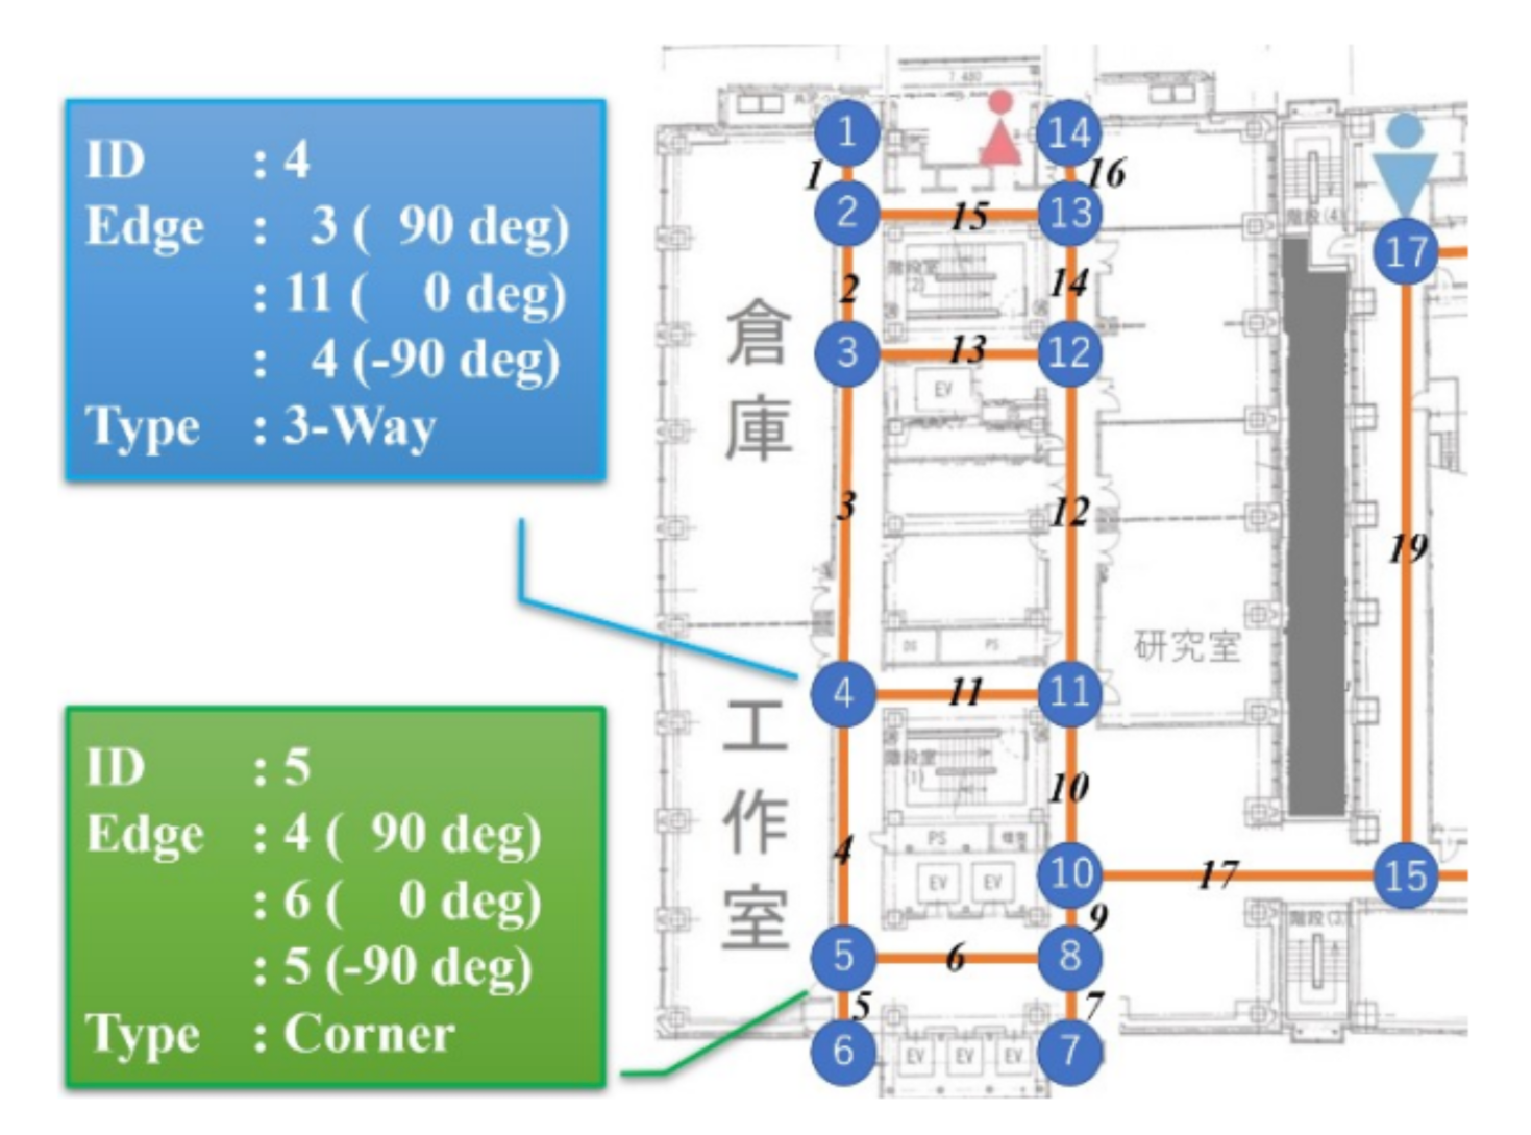
\includegraphics[width=90mm]{images/pdf/topo.pdf}
     \caption{Topological map format proposed by Shimada and others (Quoted from\cite{shimada2020})}
     \label{fig:topo}
\end{figure}
\clearpage
\subsection{シナリオ}
シナリオはトポロジカルマップ上での,目的地までの経路を単語の組み合わせで表現したものである.
具体的には,「次の角」や「突き当たりまで」のような「条件」と「直進」,「右折」のような「行動」の組み合わせにより作成される.
このシナリオの形式は,\secref{sec:shimada_topo}のトポロジカルマップと同様に人の道案内に関するアンケートを実施し
,その結果に基づいて決定された.
アンケートでは,人は「条件」と「行動」を組み合わせて道案内をしていることが明らかになっている.
例として,\figref{fig:scenario01}に示す経路をシナリオで表現すると,「3番目の三叉路まで直進.停止」となる.
\vspace{3zh}
\begin{figure}[htbp]
    \centering
     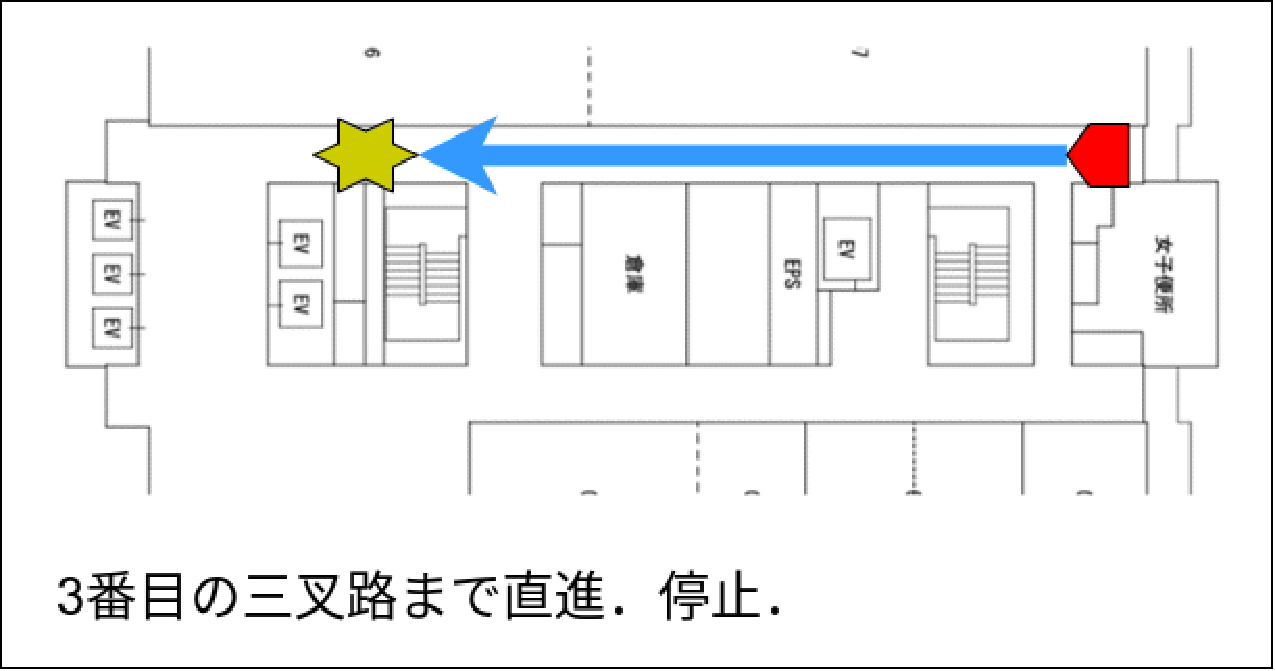
\includegraphics[width=110mm]{images/pdf/scenario/scenario01.pdf}
     \caption{Example scenarios (Quoted from \cite{haruyama2023})}
     \label{fig:scenario01}
\end{figure}
\chapter{動的に経路を選択して移動する機能の追加}
\label{chap:path_select}

\section{概要}
本章では,岡田らの従来手法に対して,目標とする進行方向のデータ
を加えることで,動的に経路を選択して移動する機能の追加を試みる.これにより,視覚に基づくナビゲーション
において,分岐路で「直進」「左折」などの任意の経路への移動
が可能となることを目指す.
以後,この動的に経路を選択して移動する機能を「経路選択機能」と呼ぶ
% \section{手法}
入力に目標方向を足した話
% \section{シミュレータを用いた実験}
シミュレータを用いて
経路選択機能の実験したよ.
% \section{実験結果}
同一の分岐路で,
選択できた

\section{経路選択機能を追加したシステム}
経路選択機能の追加を目的として,
データセットと学習器の入力へ,目標とする進行方向のデータ(以後,目標方向と呼ぶ)を新たに追加した.
\figref{fig:haru_mech_sys}に経路選択機能を追加したシステムを示す.
なお,上記の追加した要素を除き,他の部分は岡田らの従来手法と同様である.
学習時は,カメラ画像とメトリックマップに基づくルールベースの制御器から出力される
目標方向を入力としてデータセットへ加える.
岡田らの従来手法では,データセットの収集法に関して,いくつかバリエーションがある.
本論文では,その中で,最も経路追従の成功率が高い,学習器の出力とルールベース制御器の出力を比較し,
差の絶対値が閾値(0.05rad/s)を超えた場合のみ訓練データへ加える方法\cite{okada2021}を用いる.
学習後は,\figref{fig:path_select_abs}に示すように学習器へ外部から目標方向を入力する.
ロボットは視覚に基づくナビゲーションにおいて,入力された目標方向に従った経路を選択して移動する.

% 場所のデータのみ選択して訓練データに加える.
% 学習器の出力を監視して, 経路追従できない場所のデータのみ選択してデータセッ
% トに追加する手法を用いる.
\begin{figure}[htbp]
    \centering
     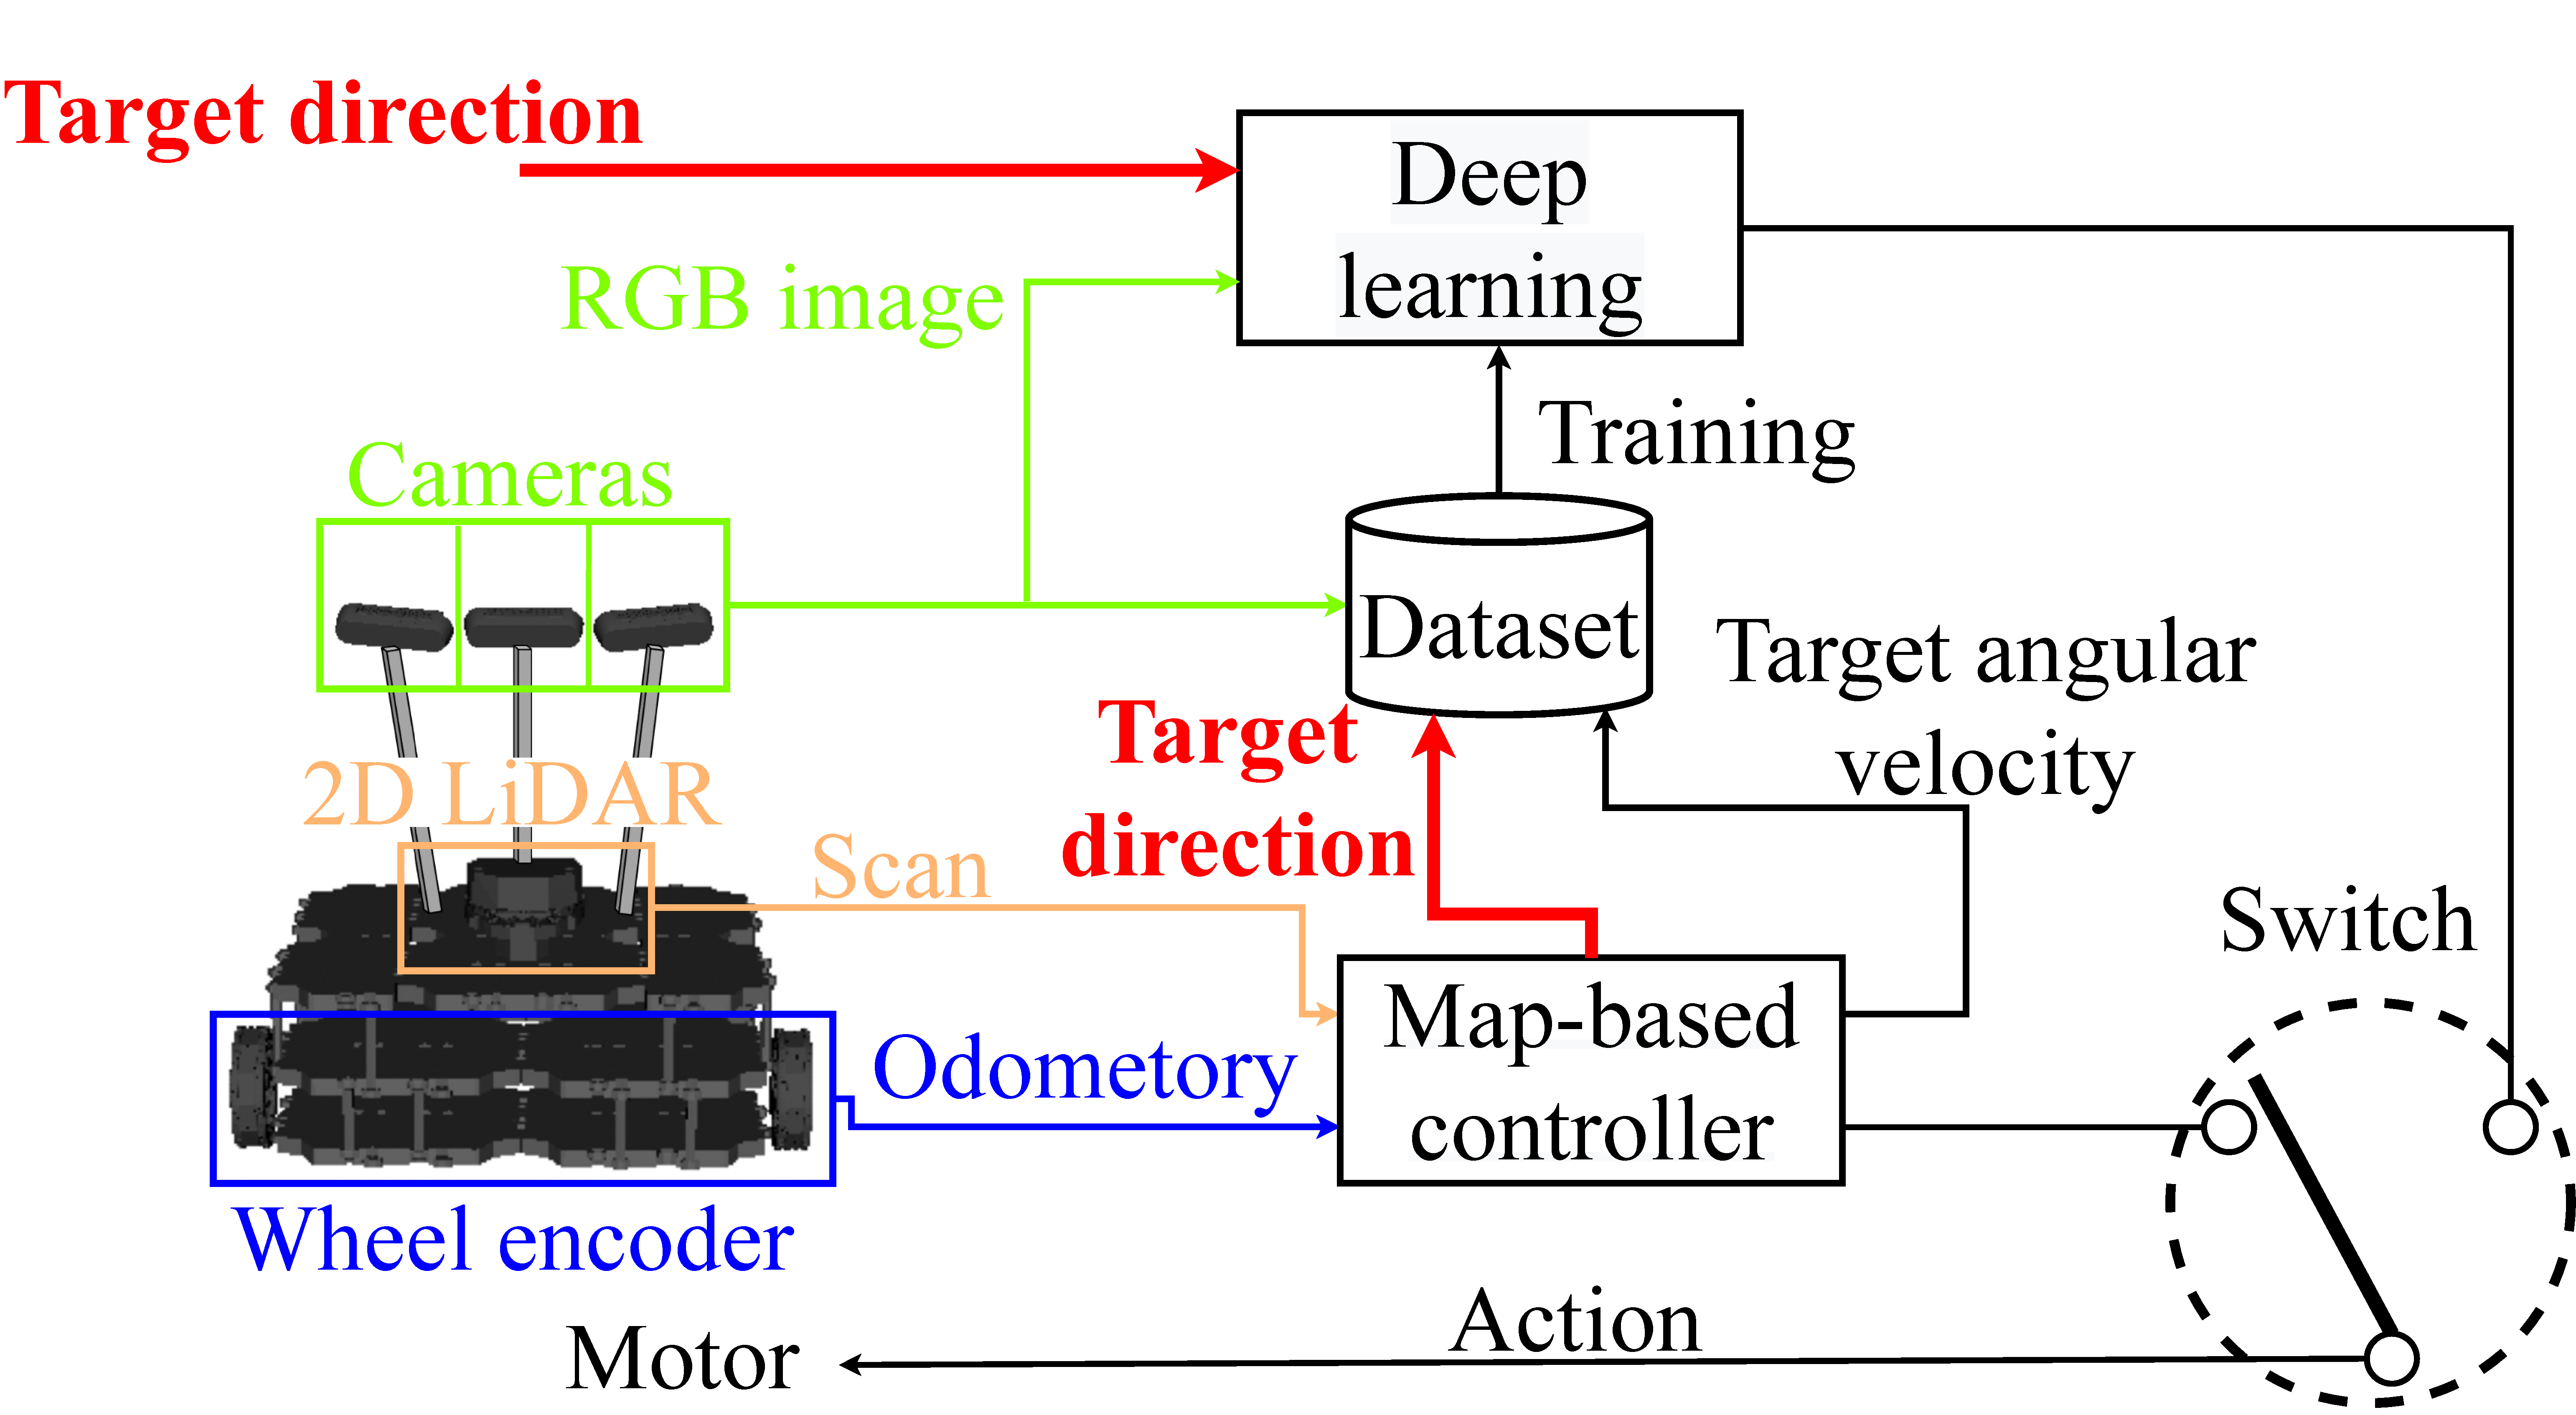
\includegraphics[width=130mm]{images/pdf/haru_mech_sys.pdf}
     \caption{System of the imitation learning with added function of
     selecting path}
     \label{fig:haru_mech_sys}
\end{figure}
\begin{figure}[htbp]
    \centering
     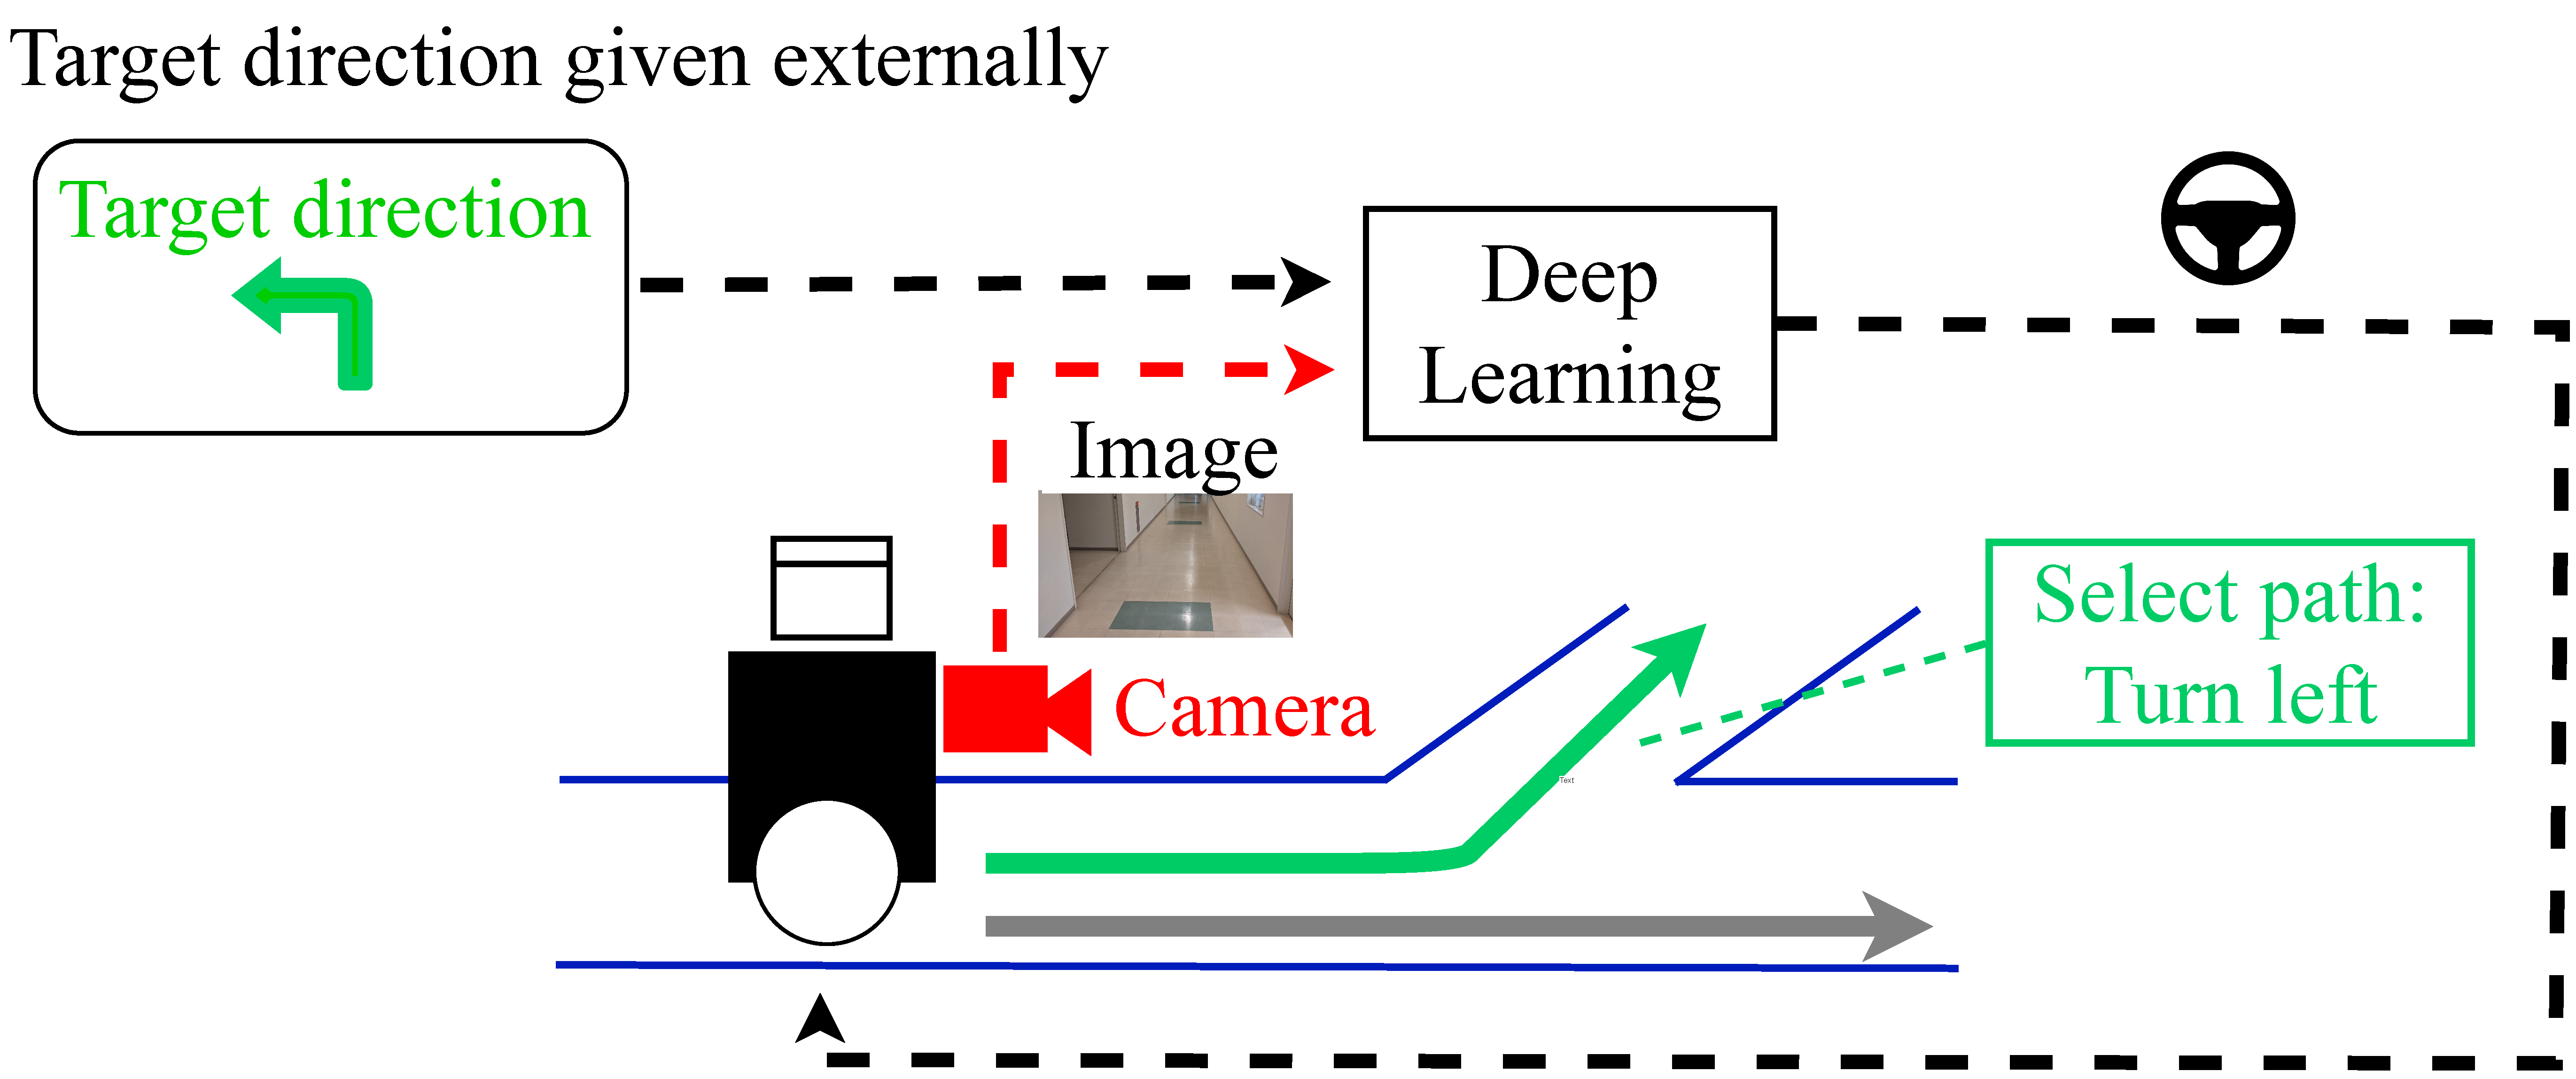
\includegraphics[width=130mm]{images/pdf/learning_gamma.pdf}
     \caption{Path selection and following behavior based on camera images 
     and target direction by imitation learning (Quoted from \cite{haruyama2023})}
     \label{fig:path_select_abs}
\end{figure}

\clearpage
\subsubsection{ネットワークの構造と目標方向のデータ形式}
経路選択機能を追加した学習器のネットワークの構造を\figref{fig:haru_mech_net}に示す.
岡田らの従来手法で用いたネットワークの出力部に,目標方向の入力部を追加した.
この層に\tabref{tab:target_old}に示すワンホットベクトルの
データを入力する.
ネットワークは,画像を処理するCNNアーキテクチャ,
CNNの出力と目標方向を入力とする全結合層で構成されている.
損失関数や活性化関数などのパラメータは岡田らの従来手法と同様である.

学習器はRGB画像と,目標方向を入力,ヨー方向の角速度を出力として
end-to-endで学習する.
つまり,視覚を入力とした行動を.目標方向によって条件付けながら学習する.
% 目標方向の
% 継続,直進,左折,右折の4つを
% ワンホットベクトルで表現する.
\begin{figure}[htbp]
    \centering
     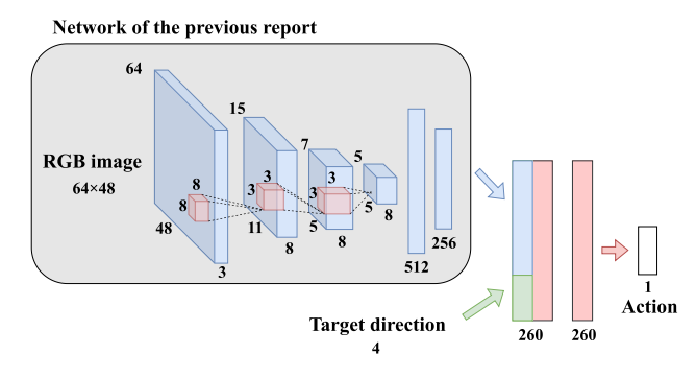
\includegraphics[width=130mm]{images/pdf/haru_mech.pdf}
     \caption{Structure of network with added function of
     selecting path}
     \label{fig:haru_mech_net}
\end{figure}

\begin{table}[htbp]
    \centering
    \caption{Target direction and data for imitation learning}\label{tab:target_old}
    \begin{tabular}{|c|c|}
    \hline
    Target direction & Data        \\
    \hline
    Continue   & {[}100,0,0,0{]} \\
    Go straight   & {[}0,100,0,0{]} \\
    Turn left   & {[}0,0,100,0{]} \\
    Turn right   & {[}0,0,0,100{]} \\
    \hline
    \end{tabular}
    \end{table}

\newpage
\section{シミュレータを用いた経路選択機能を確認する実験}
経路選択機能を追加したシステムで,指定した進行方向にロボットが移動できることを
シミュレータを用いた実験により確認する.
\subsubsection{実験装置}
実験はシミュレータ上で行い,シミュレータにはGazebo\cite{Gazebo}を使用し,
ロボットには\figref{fig:turtlebot3}に示すTurtleBot3 Waffle Pi\cite{ROBOTIS}へ3つのカメラを追加したモデルを用いる.
実験環境には,\figref{fig:haru_mech_exp}に示す千葉工業大学津田沼キャンパス2号館3階を模したモデルを用いた.
環境中のA,Bの地点においては,\figref{fig:haru_mech_exp_ab}に示すように侵入する方向が3つ,脱出する経路はそれぞれ2つ
あるため,バリエーションは6つある.
つまり,目標方向に従って適切に経路を選択して移動することが求められる場所となる
\begin{figure}[htbp]
    \centering
     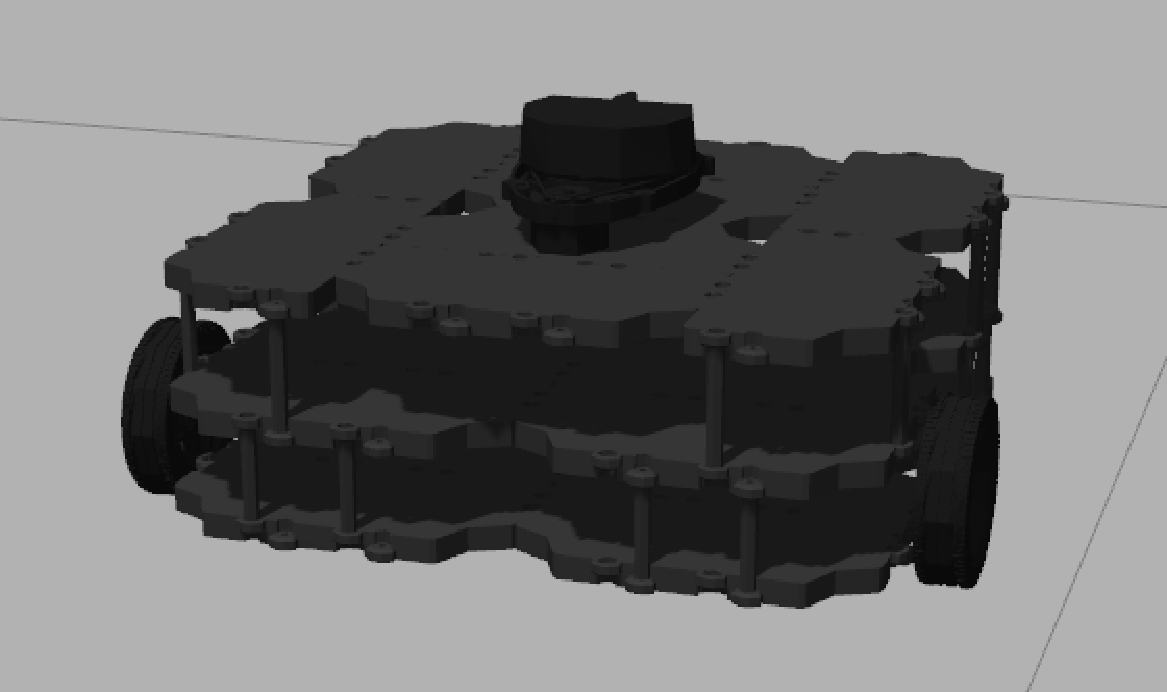
\includegraphics[width=80mm]{images/pdf/turtlebot3.pdf}
     \caption{TurtleBot3 Waffle Pi}
     \label{fig:turtlebot3}
\end{figure}
\begin{figure}[htbp]
    \centering
     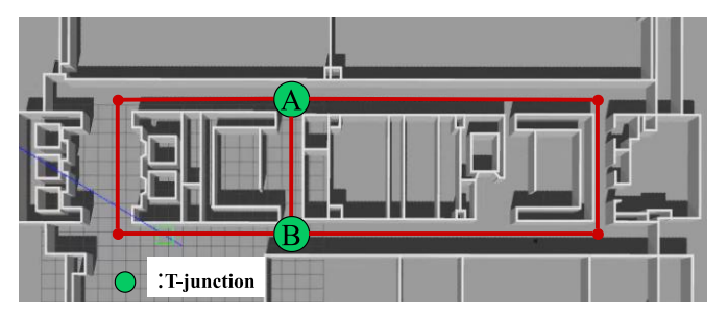
\includegraphics[width=130mm]{images/pdf/haru_mech_exp.pdf}
     \caption{Experimental environment of selecting path (Quoted from \cite{haruyama2022})}
     \label{fig:haru_mech_exp}
\end{figure}
\begin{figure}[htbp]
    \centering
     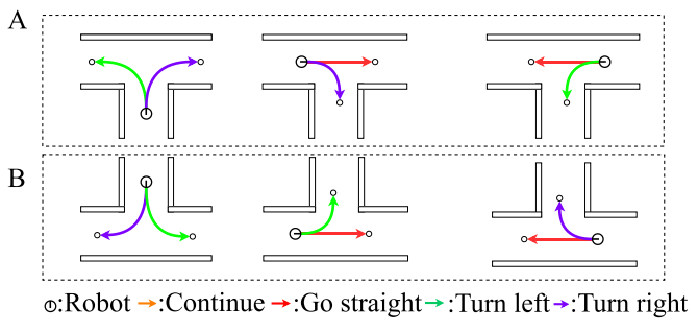
\includegraphics[width=130mm]{images/pdf/haru_mech_exp_ab.pdf}
     \caption{Selecting a path at the T-junction (Quoted from \cite{haruyama2022})}
     \label{fig:haru_mech_exp_ab}
\end{figure}
\vspace{-1zh}
\subsubsection{実験方法}
実験は,\figref{fig:haru_mech_route}に示した経路をaからfの順番で繰り返し走
行しながら,模倣学習を行う.目標方向のデータはメトリックマップに基づくルールベース制御器から出力
され,データセットに加えられる.学習は60000ステップ実行し,
その後視覚に基づくナビゲーションへ移行する.視覚に基づくナビゲーションにおいても
aからfまでの経路をロボットに走行させる.ロボットが壁に衝突した場合は,
ロボットを経路の中央まで戻して実験を継続する.
この実験を10回実施する.

\begin{figure}[htbp]
    \centering
     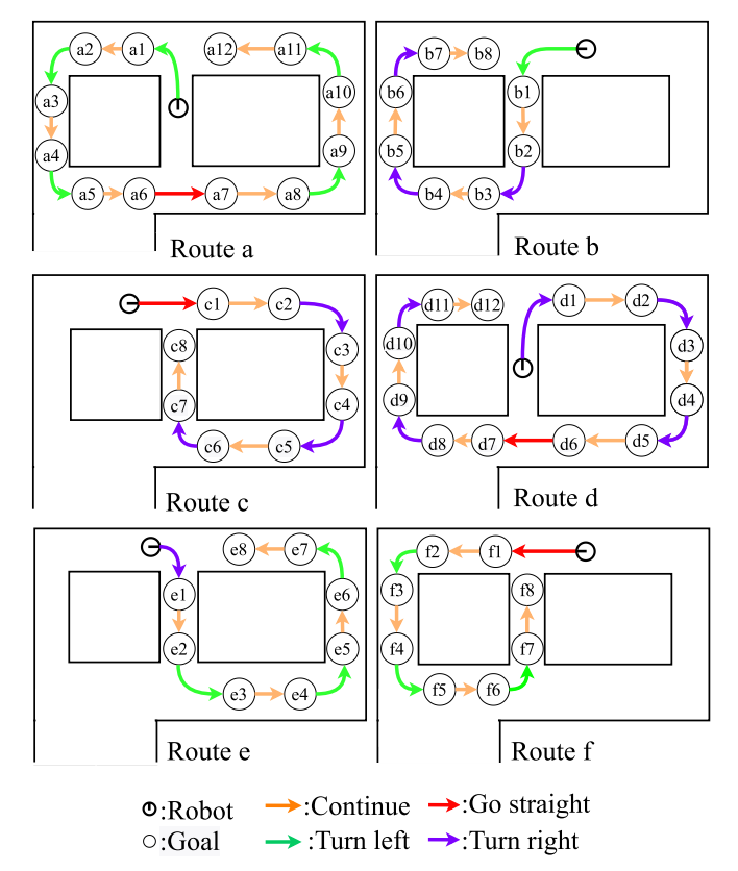
\includegraphics[width=130mm]{images/pdf/haru_mech_route.pdf}
     \caption{Route for experiment of selecting path (Quoted from \cite{haruyama2022})}
     \label{fig:haru_mech_route}
\end{figure}
\clearpage
\subsubsection{実験結果}
実験結果を\figref{fig:haru_mech_ab_res}に示す.
図はA,Bそれぞれの分岐路で,ロボットが正しく経路を選択した回数を示している.
図に示すように,目標方向に従い113/120回適切に経路を選択する様子が
確認できた.ただし,\tabref{tab:path_res}に示した箇所では,壁に衝突するな
どして自律移動が継続できない様子も見られた.

\figref{fig:haru_mech_a_select}にA地
点で目標方向のコマンドに従い,ロボットが経路を選択して
走行する様子を示す.このように,同一の分岐路であっても目
標方向の入力に従い,ロボットが適切に経路を選択して走行
する様子が見られた.
この結果から,岡田らの従来手法に対し,任意の目的地に向けた移動に必要な,動的に経路を選択した移動する機能を
追加できたと考えられる,
% \vspace{5zh}
\begin{figure}[htbp]
    \centering
     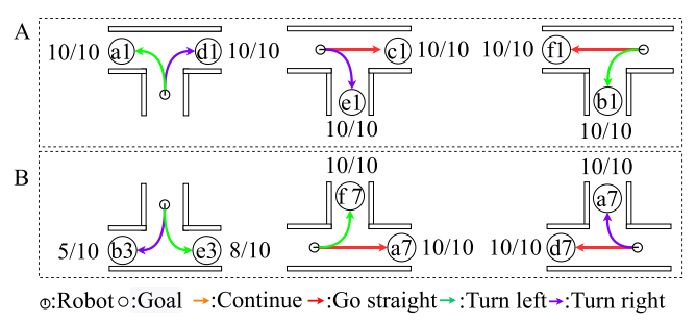
\includegraphics[width=130mm]{images/pdf/haru_mech_res.pdf}
     \caption{Number of times a correct path was selected (Quoted from \cite{haruyama2022})}
     \label{fig:haru_mech_ab_res}
\end{figure}
\vspace{-1zh}
\begin{table}[htbp]
    \centering
    \caption{Location where the robot went off course}\label{tab:path_res}
    \begin{tabular}{|c|c|c|}
    \hline
    Location & Number of Failed        \\
    \hline
    a5   & 2/10 \\
    b3   & 5/10 \\
    d11   & 1/10 \\
    e1  &  2/10 \\
    f5    & 2/10 \\
    \hline
    \end{tabular}
    \end{table}
\begin{figure}[htbp]
    \centering
    %  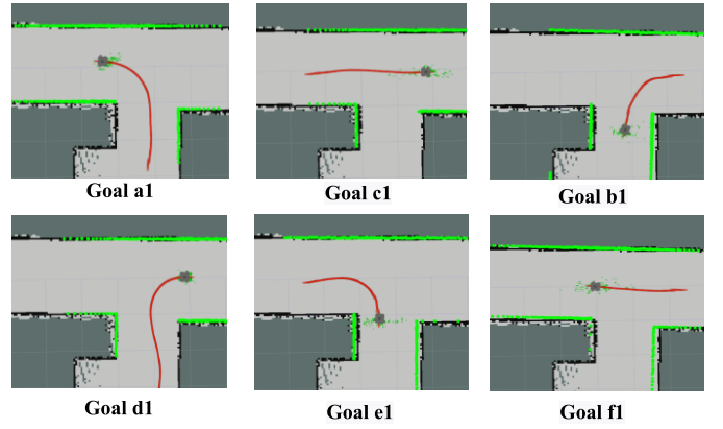
\includegraphics[width=120mm]{images/pdf/haru_mech_a_select.pdf}
     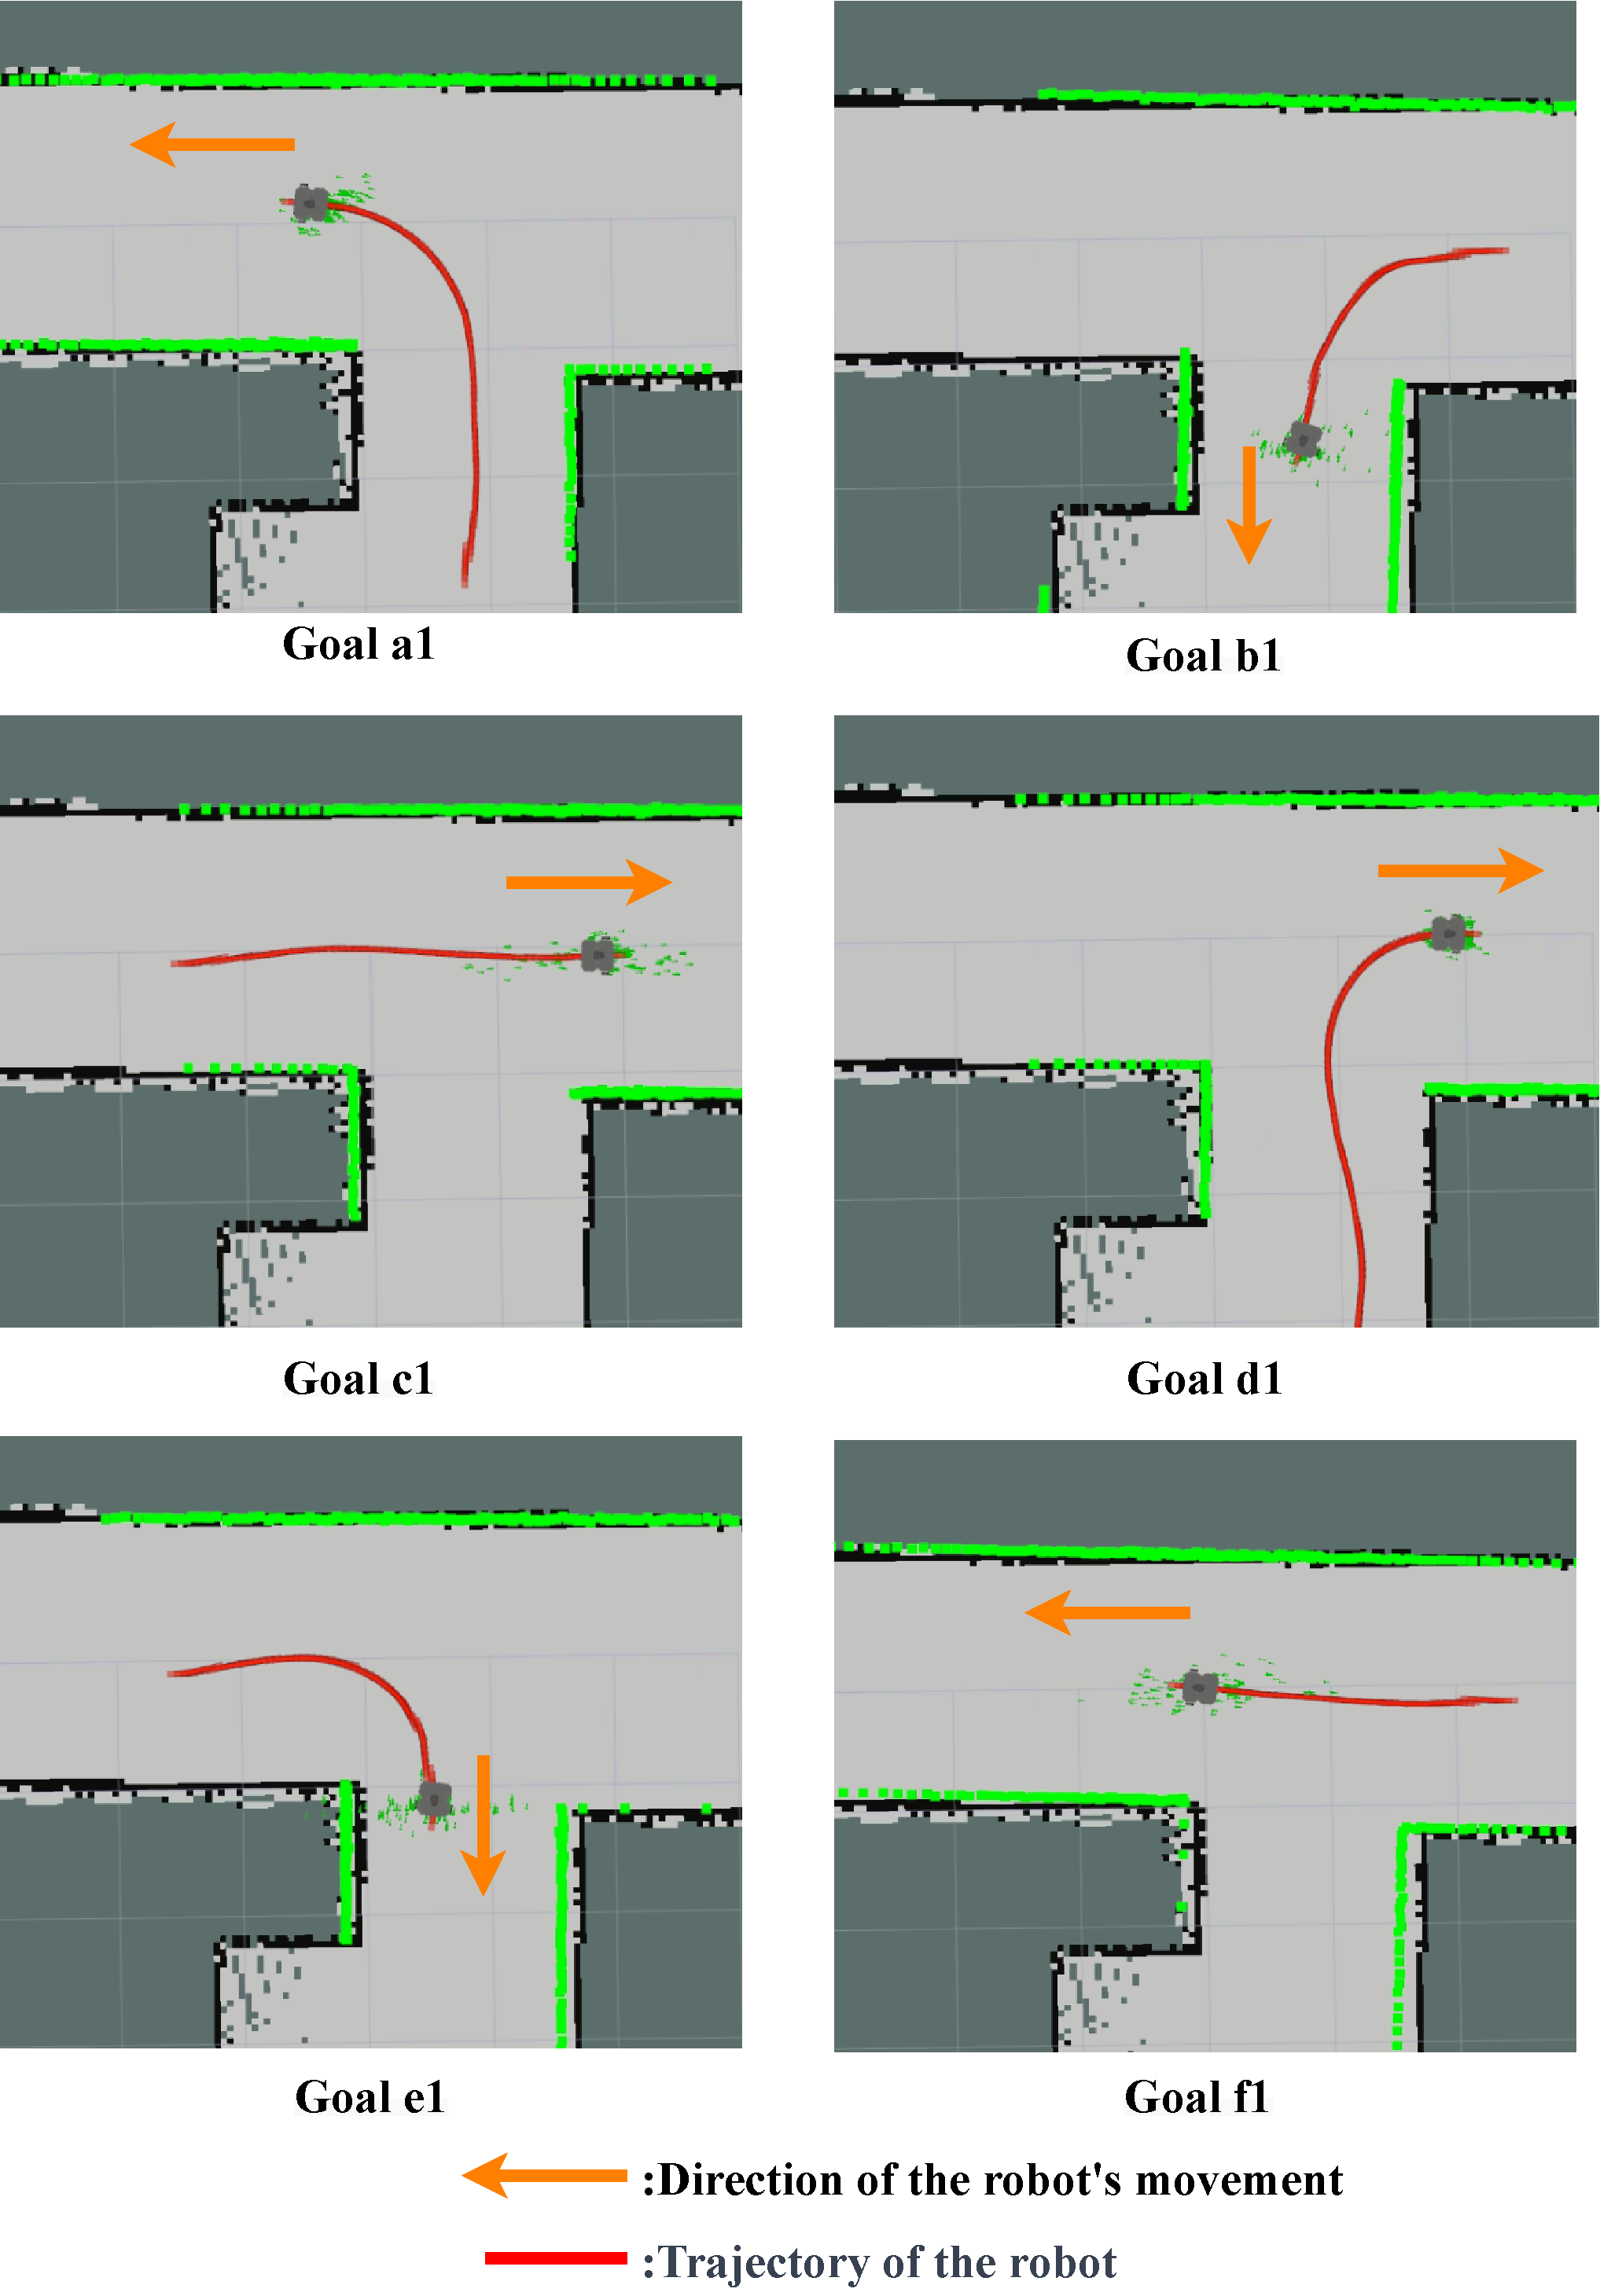
\includegraphics[width=130mm]{images/pdf/zyuziroute-select_a.pdf}
     \caption{The robot moving while selecting a path (Quoted from \cite{haruyama2022})}
     \label{fig:haru_mech_a_select}
\end{figure}

\chapter{視覚に基づいて目的地まで自律移動するシステムの構築}
\label{chap:scenario_vision}
\chapref{chap:path_select}では岡田らの従来手法に対し,経路選択機能を追加した.
これにより視覚に基づくナビゲーションにおいて,
分岐路で目標方向の入力に従った経路を選択して移動できることを確認した.
本章では,視覚に基づいて通路の特徴を検出する機能,目標方向を提示する機能を追加する.
% 目的の分岐路へ到達することを視覚から判断する機能を\secref{sec:intersection},
% 分岐路において目標方向を指示する機能を\secref{sec:scenario}で述べる.
目標方向の提示には島田ら\cite{shimada2020}が提案したトポロジカルマップとシナリオを用いる.
これにより,カメラ画像とトポロジカルマップから作成されるシナリオに基づいて,
目的地まで自律移動するシステムを構築する.
% また,このシステムにより事前に作成したメトリックマップを必要せずに,
% カメラ画像を入力として目的地まで自律移動できる可能性がある.
% 構築するシステムでは,人間が作成した「次の角まで直進.左折.」などのシナリオから
% 指示された道順に従い,カメラ画像に基づいて目的地まで自律移動する.
% で提案するシステムの概要と一連の内容を述べた後,システムを構成する
% モジュールについて詳細に述べる.
%
%\input{introduction/preface}
%
\section{構築したシステムの概要}
構築したシステムでは,人間が作成した
「次の角まで直進.左折.」などのシナリオから指示された道順に従い,カメラ画像に基づいて目的地まで自律移動する.
\figref{fig:abs}に構築したシステムの概要と自律移動の流れを示す.
構築したシステムは\\
1)シナリオを分解し,「条件」と「行動」を抽出するモジュール(以後,シナリオモジュールと呼ぶ)\\
2)カメラ画像と目標方向に基づいて,経路を追従するモジュール(以後,経路追従モジュールと呼ぶ)\\
3)カメラ画像を基に通路の特徴を分類するモジュール(以後,通路分類モジュールと呼ぶ)\\
% 〜で述べるシナリオモジュールと
% 〜で述べる経路追従モジュール
% 〜で述べる通路分類モジュールの
3つのモジュールで構成されている.
ロボットはaからdの一連の流れにより指示された道順に従って目的地まで自律移動する.
\vspace{3zh}
\begin{figure}[htbp]
    \centering
     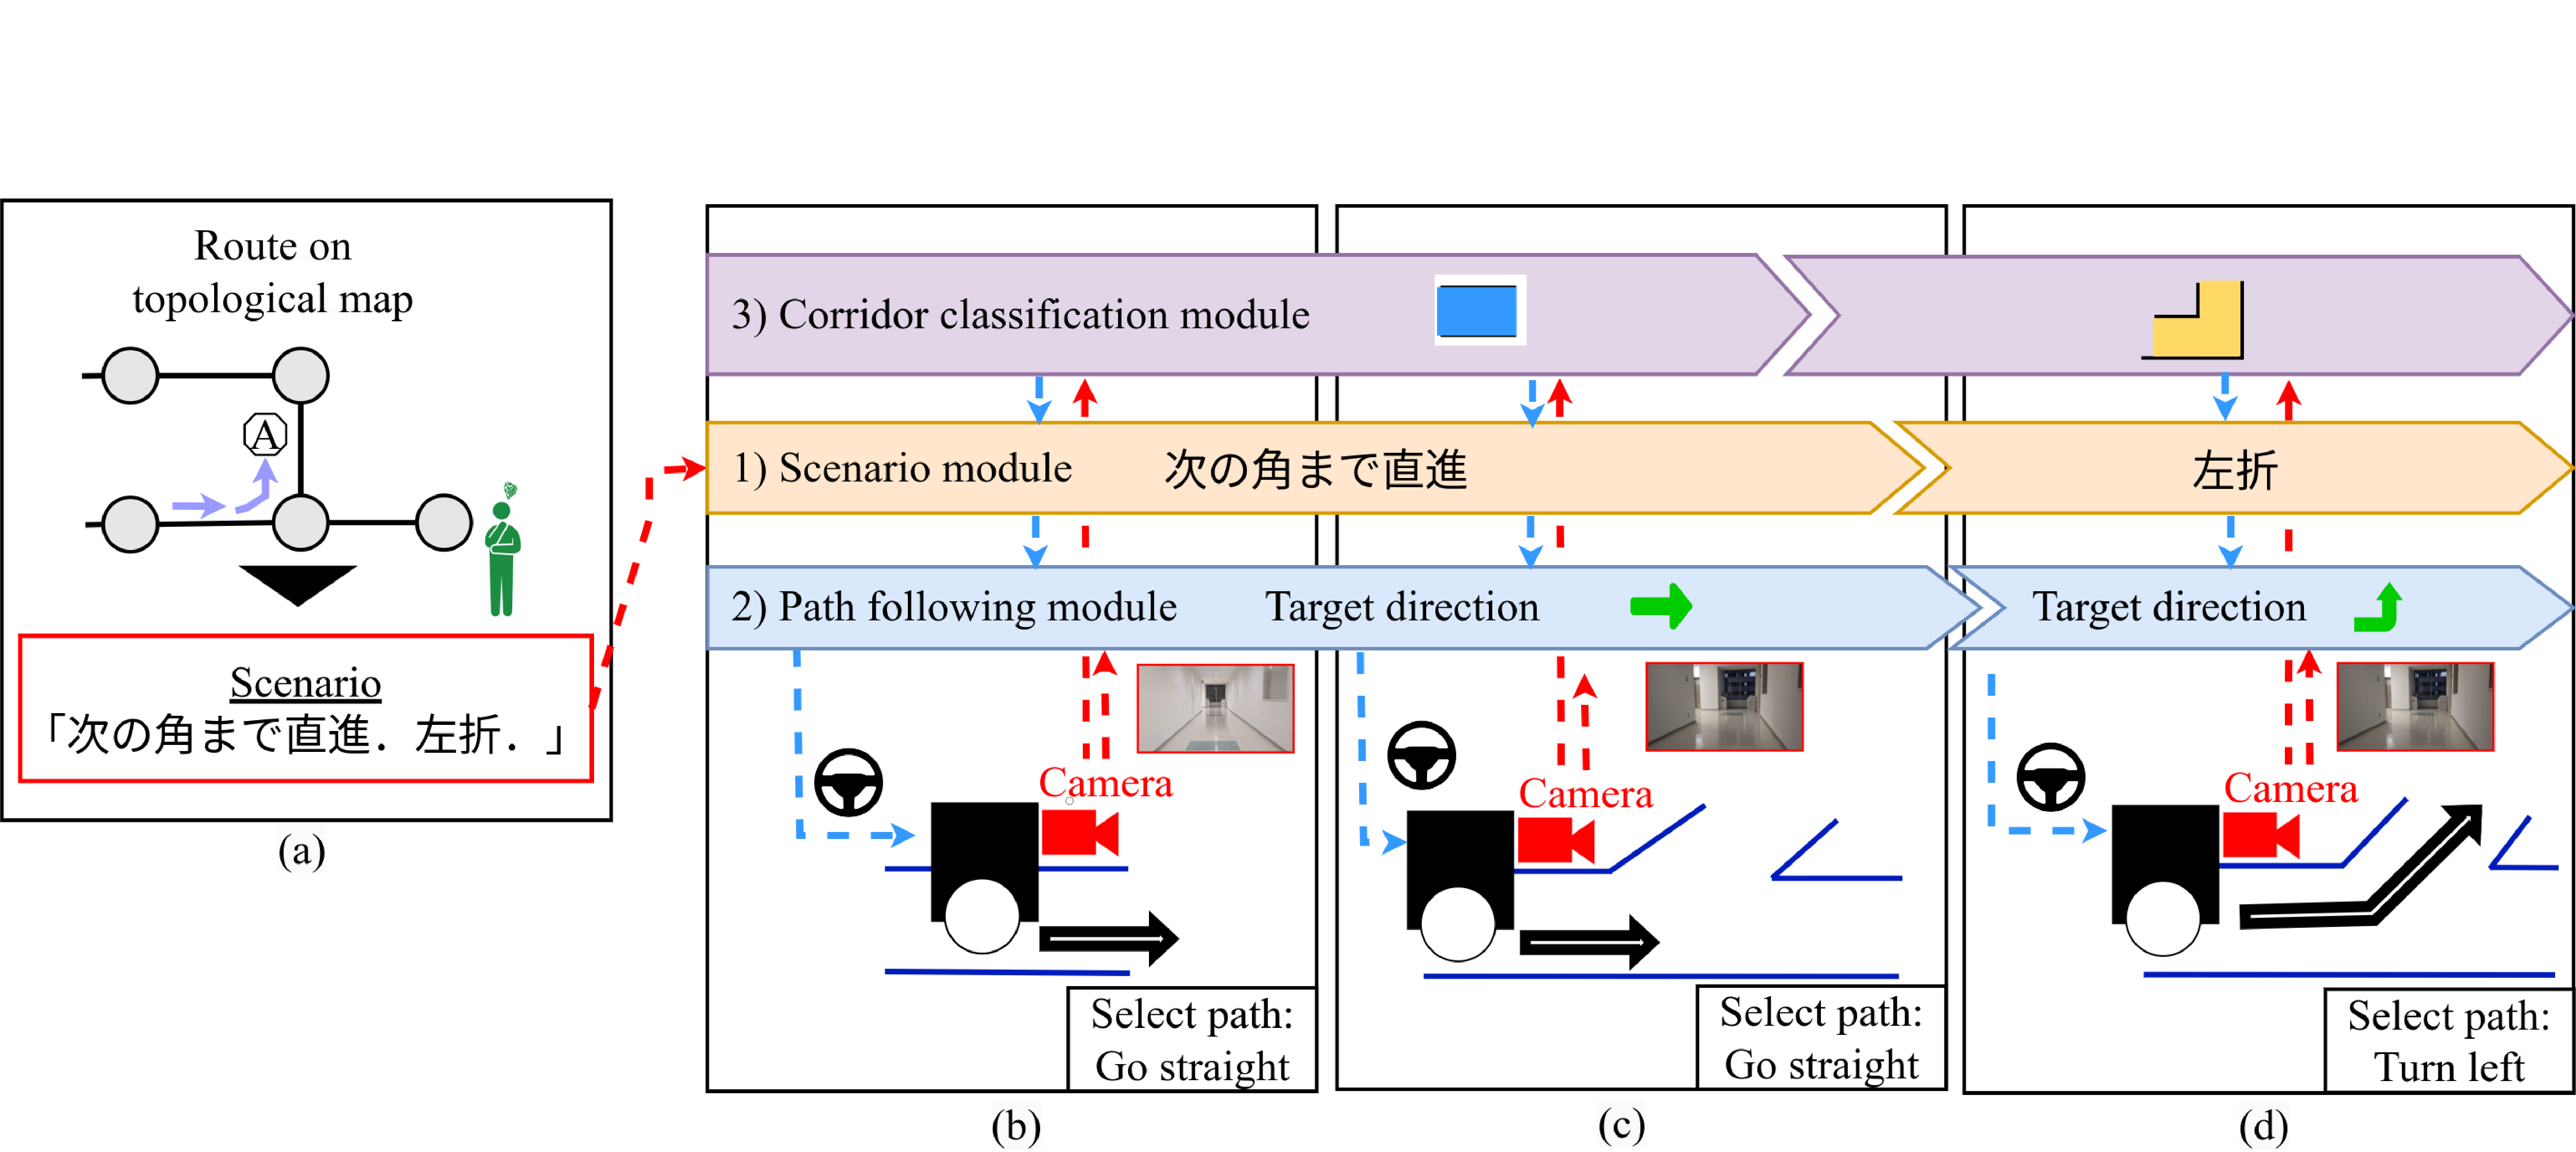
\includegraphics[width=130mm]{images/pdf/absv3.pdf}
     \caption{Overview of constructed system (Quoted from \cite{haruyama2023})}\label{fig:abs}
\end{figure}
\begin{enumerate}
    \item [(a)] トポロジカルマップ上の目的地に応じて,
    人間が「条件」と「行動」で構成されるシナリオを作成する.
    例えば,図のトポロジカルマップ上でAを目的地とするシナリオは「次の角まで直進.左折.」となる.
    \item [(b)] 作成したシナリオをシナリオモジュールへ入力する.
    シナリオモジュールは入力されたシナリオを分解し,「条件」と「行動」を抽出する.
    1つ目の条件と行動のセットは「次の角まで」と「直進」となる.
    この「直進」を目標方向として経路追従モジュールへ与える.
    経路追従モジュールは,カメラ画像と与えられた
    目標方向に基づいて,経路に沿って直進する.
    \item [(c)] ロボットが角に近づくと,
    % 通路分類モジュールの分類結果が角となり,
    通路分類モジュールがカメラ画像に基づいて
    通路を「角」と分類して,それをシナリオモジュールに与える.
    シナリオモジュールはそれを基に「次の角まで」という条件を満たしたかを判定する.
    この場合は条件を満たしているため,2つ目の行動である「左折」
    へ遷移する.
    \item [(d)]「左折」に基づいて,経路追従モジュールは
    経路に沿って角を左折する.
\end{enumerate}

% なお3つのモジュールはRobot Operating System(以下,ROS)\cite{ros}のフレームワーク上で作成している.
% また,通路分類モジュールと経路追従モジュールでは
% 機械学習のフレームワークとしてpytorch\cite{torch}を使用している

\newpage
\section{経路追従モジュール}
\label{sec:imitation}
経路追従モジュールについて述べる.
このモジュールは\ref{chap:path_select}章で述べたシステムに倣って構築した,
カメラ画像に基づいて経路を追従するモジュールであり,
分岐路では入力された目標方向によって経路を選択して走行する.
なお,\ref{chap:path_select}章で述べたシステムに対し,
目標方向とネットワークのパラメータ変更,データセットの収集方法の追加をしている.

% 次に追加した,データセットの収集方法について述べる.
% \ref{chap:path_select}章では,学習器の訓練に60000stepを必要とし,
% 実ロボットを用いた実験に向けて,必要となる学習の量を削減することが望まれる.
% 藤原らが提案する
% データセットに加えるデータの不均衡を改善する手法
% 学習時に積極的に蛇行する手法
% 次に
% \ref{fig:learning_sys}に経路追従モジュールのシステムを示す.


% 学習時は,2D-LiDARやオドメトリ,
% 事前に作成したメトリックマップに基づいた
% ルールベース制御器(ROS Navigation stack)によって,設定した経路を追従する.
% その際,入力をカメラ画像と目標方向,
% 出力をヨー方向の角速度とするデータを,0.2秒周期でデータセットに加える.
% このヨー方向の角速度はメトリックマップに基づいたルールベース制御器が
% 出力する信号である.カメラ画像の収集では
% 中央, 左,右に傾けて取り付けた3つのカメラを用いる.
% 左と右のカメラ画像に対する角速度には,経路に戻るようにオフセットを加える.
% さらに,バッチサイズを8として
% 教師データを抽出し,0.2 秒の周期でオンラインで学習する.
% このデータセットへのデータの追加から学習までの1連の流れを1ステップとする.
% 学習時のデータセットへ加える目標方向には,
% メトリックマップに基づいたルールベースの制御器からの出力を用いる.

% 学習後,モジュールはカメラ画像と目標方向を基に,
% 出力したヨー方向の角速度により経路を追従する.
% このとき,並進速度は 0.2m/s である.
% なお,目標方向が「停止」の場合は,0.0m/s となる.
% \begin{figure}[htbp]
%     \centering
%      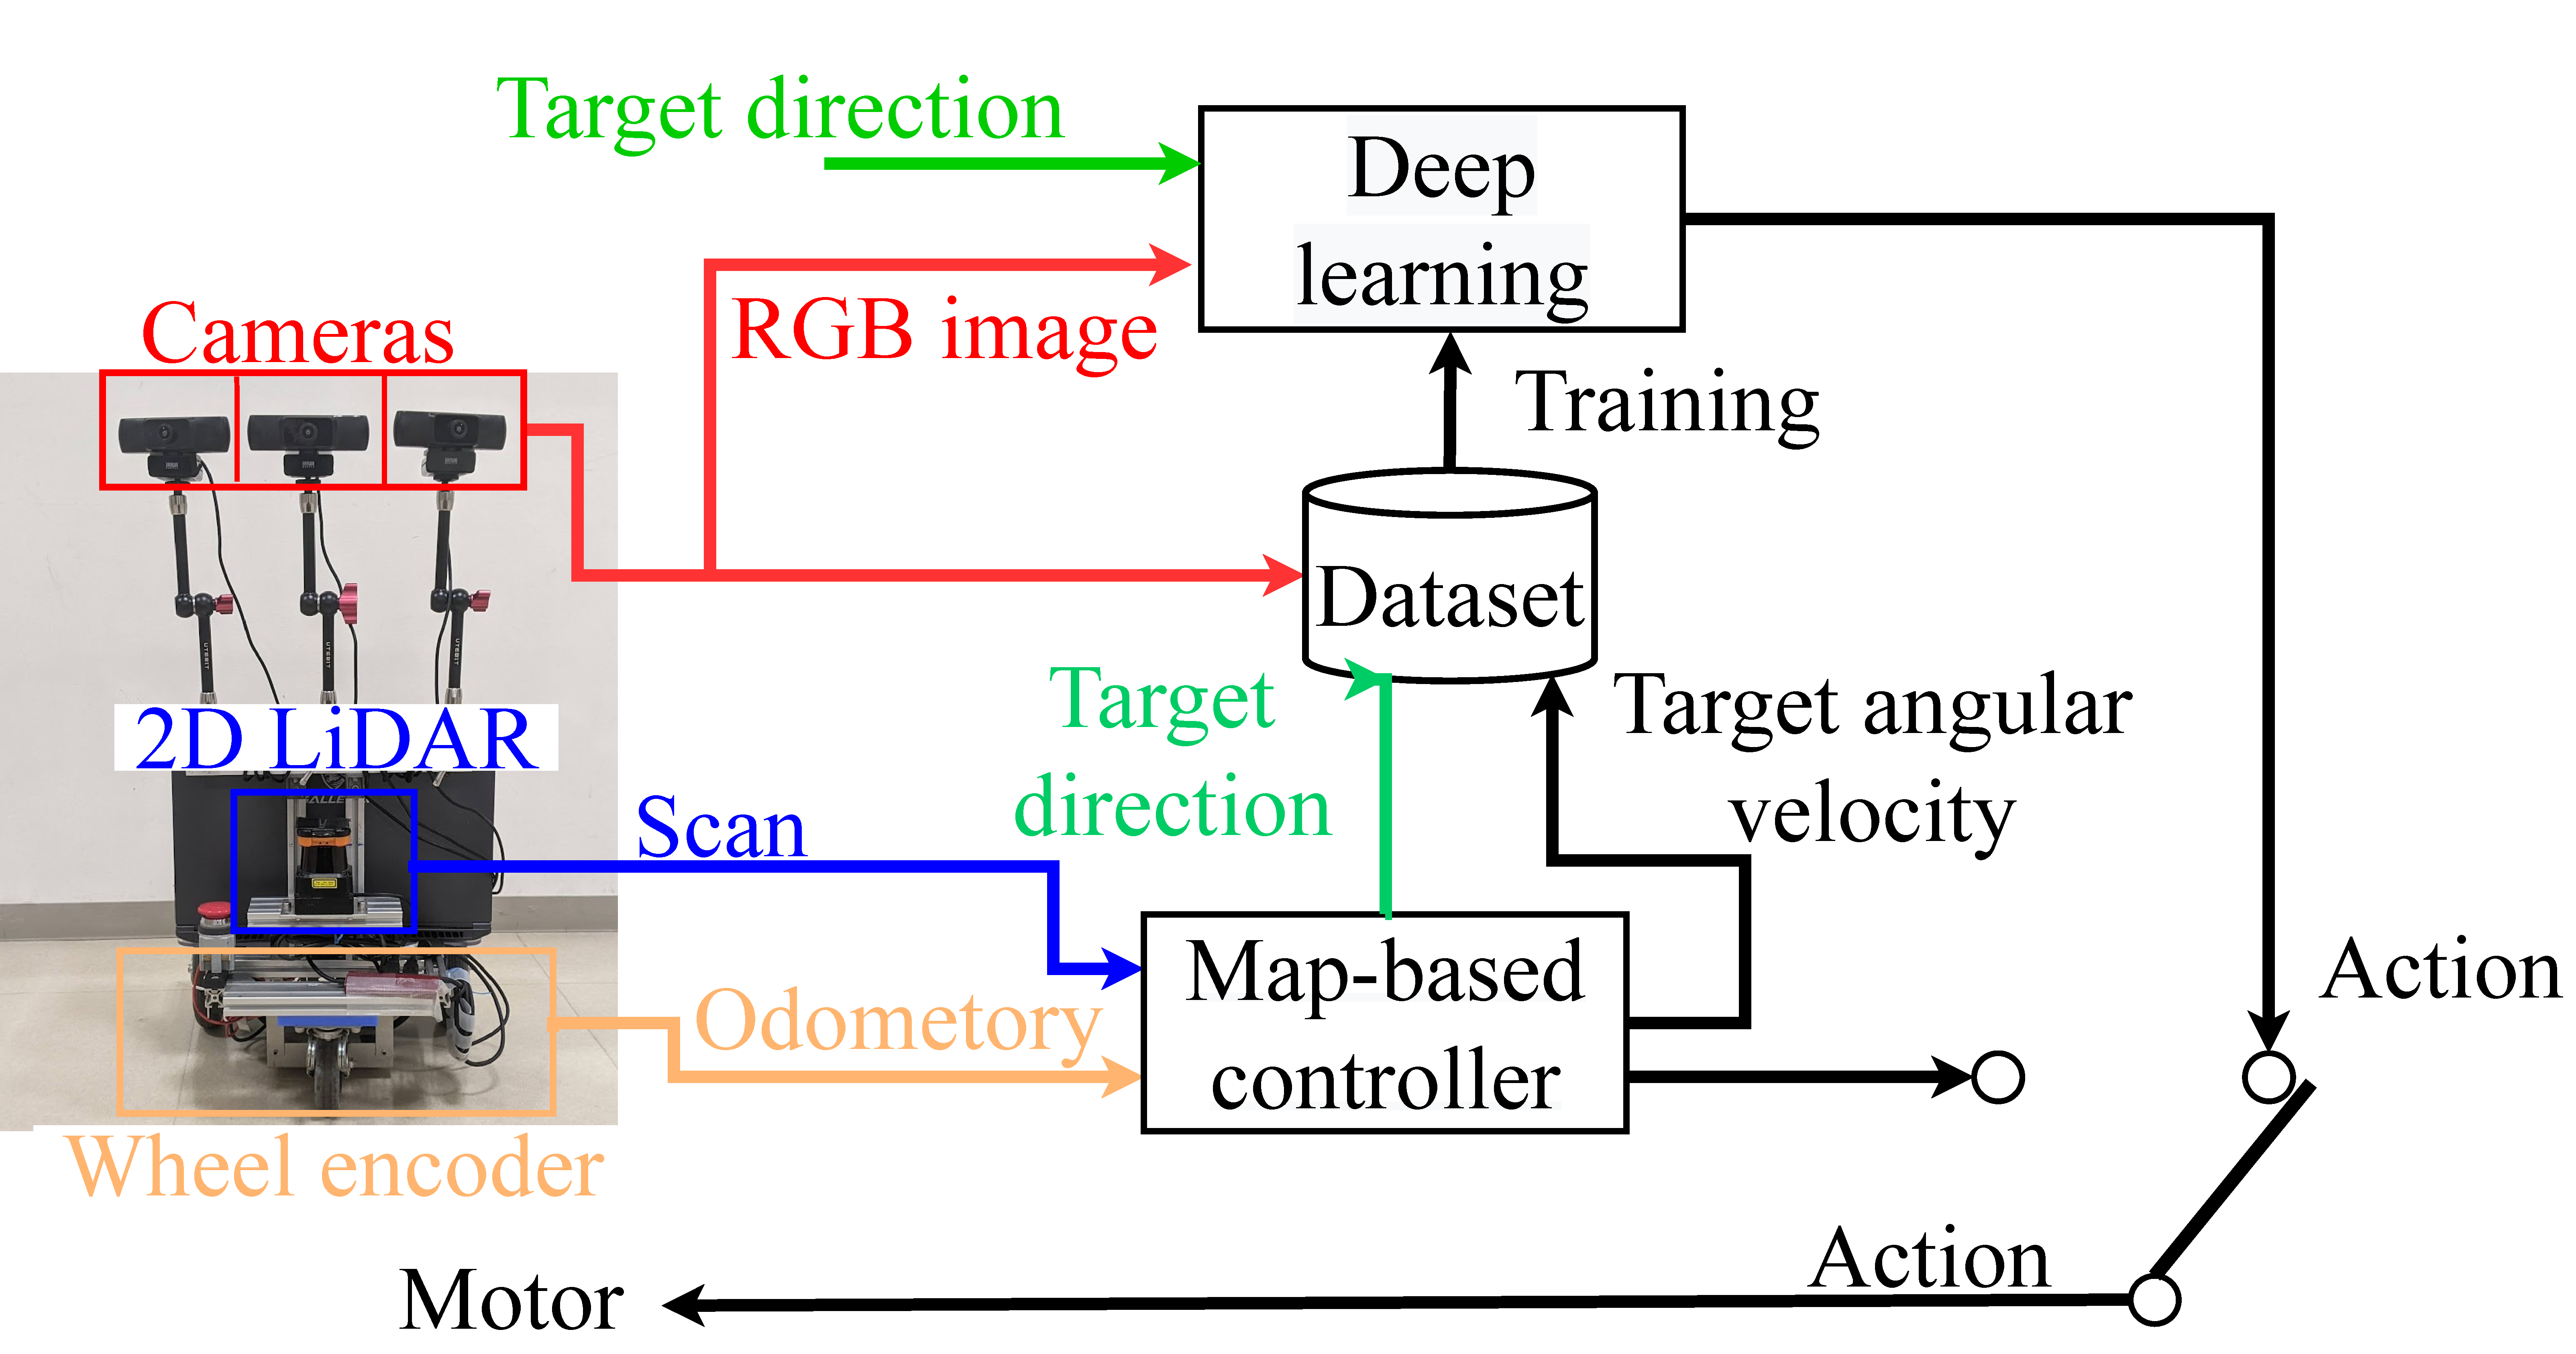
\includegraphics[width=130mm]{images/pdf/system_learning.pdf}
%      \caption{Path-following module system}\label{fig:learning_sys}
% \end{figure}

追加した学習時のデータセットの収集方法は,
% % 岡田ら\cite{okada2021}が提案した
% % \begin{quote}
% %     \begin{itemize}
% %      \item 学習器の出力を監視して,経路追従できない場所のデータのみ選択してデータセ
% %      ットに追加する手法
% %     \end{itemize}
% %    \end{quote}
% の他に
藤原ら\cite{fujiwara2023}が学習量の削減を目的に行った以下の2つの手法である.
\begin{quote}
    \begin{itemize}
     \item データセットに加えるデータの不均衡を改善する手法
     \item 学習時に積極的に蛇行する手法
    \end{itemize}
   \end{quote}


データセットに加えるデータの不均衡を改善する手法について述べる.
\figref{fig:oversmple}に,\chapref{chap:path_select}の実験における10000ステップあたりの目標方向
を青で示す.直進のデータが他に比べ圧倒的に多く,不均衡あることが分かる.
Haiboらの調査\cite{hukinko}では,ほとんどの標準的な学習アルゴリズムは,データの不均衡によりパフォー
マンスが大幅に低下するとされている.
そこで,データ前処理手法であるオーバーサンプリングを用いて,データの偏りを改善する.
具体的には,図中赤で示すように左折と右折を7倍に複製する.
\vspace{3zh}
\begin{figure}[htbp]
    \centering
     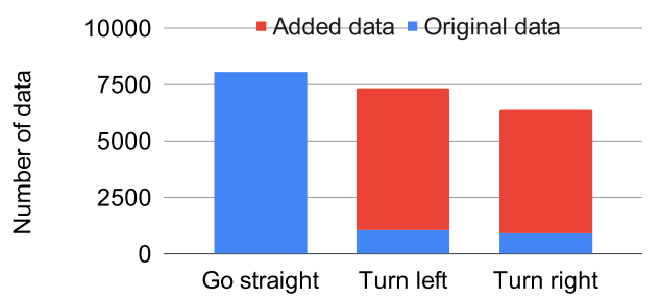
\includegraphics[width=100mm]{images/pdf/oversmple.pdf}
     \caption{Number of data in the target direction per 10000 steps
     in the previous experiment Quote from \cite{fujiwara2023}}\label{fig:oversmple}
\end{figure}
\clearpage
次に,学習時に積極的に蛇行する手法について述べる.
学習時に経路から離れた状態が増加すると,訓練済みの学習器での走行時に経路から
外れることが減少し,より少ない学習時間で成功率が高いモデルができる可能性がある.
そのため,学習時に積極的に蛇行する手法では\figref{fig:dakou}に示すように,
学習時のロボットの制御に用いるヨー方向の角速度を1.5倍にする.
これにより,大きく蛇行して,目標経路から離れた状態を多く収集する.

藤原らは実験により,これらの2つのデータセットの収集手法によって,
経路追従の成功率を下げること無く,必要な学習量を60000ステップから
20000ステップまで削減できることを確認している.
\begin{figure}[htbp]
    \centering
     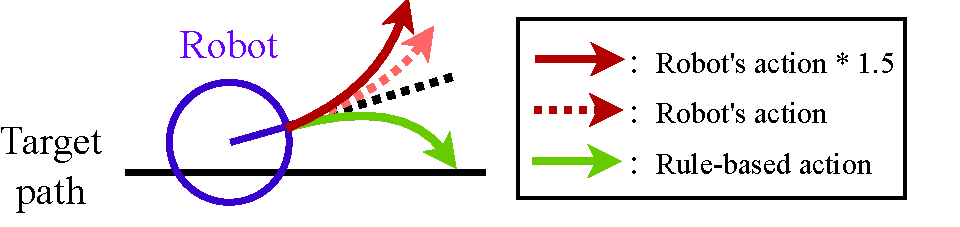
\includegraphics[width=130mm]{images/pdf/dakou.pdf}
     \caption{Aggressive meandering (Quote from \cite{fujiwara2023})}\label{fig:dakou}
\end{figure}
\newpage

\tabref{tab:target}に変更した目標方向とそのデータ形式を示す.
\chapref{chap:path_select}における
目標方向の中で,ContinueとGo straightは同じ方向を指しているため,本章ではこれらを1つとして扱う.
これに伴い,ワンショットベクトルの次元数を4から3へ変更している.
さらに,目的地に到着後,ロボットを停止させることを目的として,
Stop(停止)の目標方向を追加した.
停止の目標方向が入力された際には,ロボットの並進速度は0.0m/sとなり,ロボットはその場で停止する.
% なお,停止以外の目標方向における並進速度は\chapref{chap:path_select}と同様に0.2m/sである.
% 「停止」が入力された場合は0.0m/sとなる.

目標方向の次元数に伴い,変更を加えたネットワークの構造を\figref{fig:imi_net}に示す.
具体的には,CNNの出力と目標方向を入力する全結合層の入力サイズを260から259へ調整している.

\begin{table}[htbp]
    \centering
    \caption{Target direction and data for path-following module}\label{tab:target}
    \begin{tabular}{|c|c|}
    \hline
    Target direction & Data        \\
    \hline
    Go straight   & {[}1,0,0{]} \\
    Turn left   & {[}0,1,0{]} \\
    Turn right   & {[}0,0,1{]} \\
    Stop   & {[}0,0,0{]}\\
    \hline
    \end{tabular}
    \end{table}
% 経路追従モジュールで用いるネットワークの構造を\ref{fig:imi_net}に示す.
% ネットワークはRGB画像と,目標方向を入力,ヨー方向の角速度を出力として
% end-to-endで学習する.
% ネットワークは,画像を処理するCNNアーキテクチャ,
% CNNの出力と目標方向を入力とする全結合層で構成されている.
\begin{figure}[htbp]
    \centering
     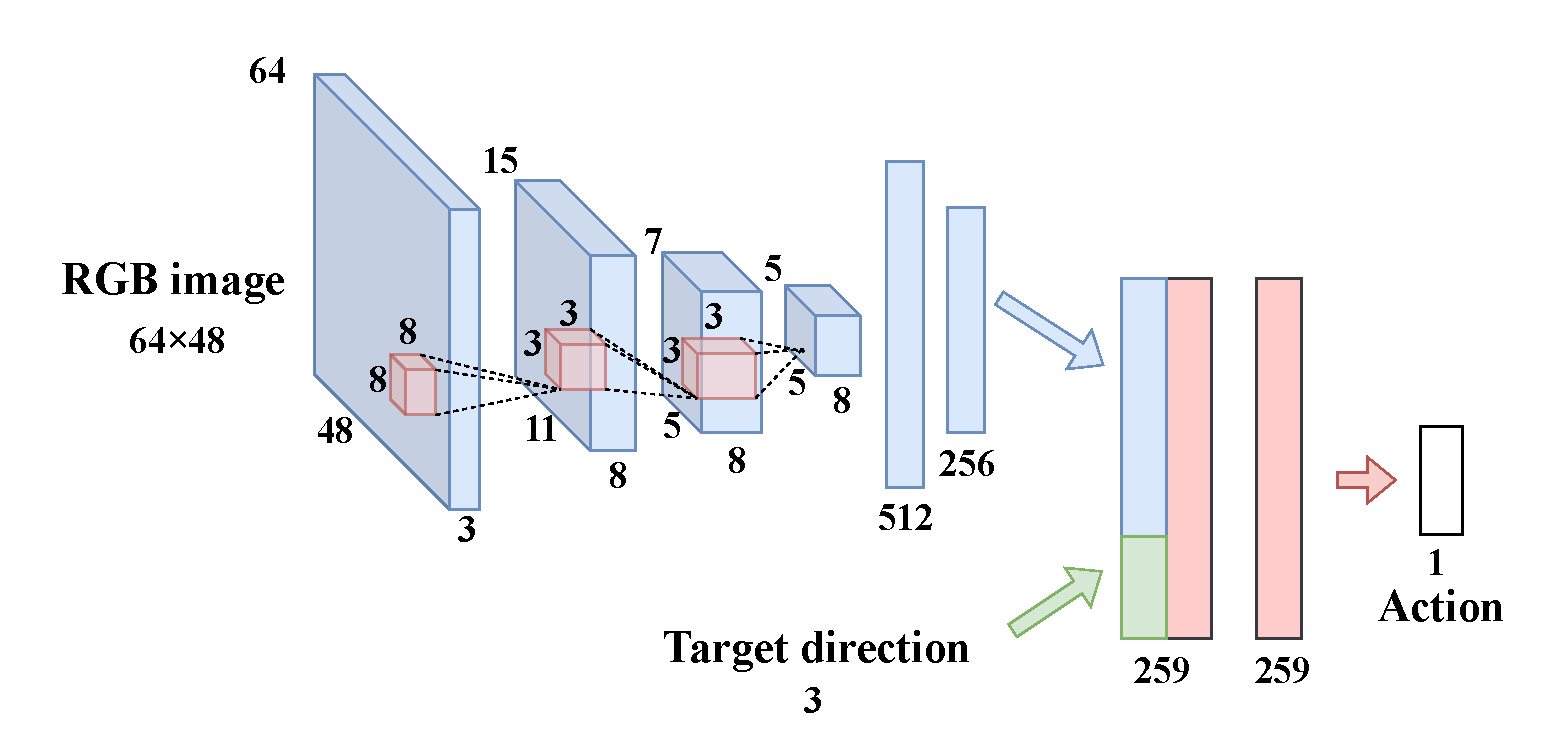
\includegraphics[width=130mm]{images/pdf/imi_net.pdf}
     \caption{Structure of the network of route selection module}
     \label{fig:imi_net}
\end{figure}

% 目標方向は\ref{tab:target}に示す
% 直進,左折,右折の3つをワンホットベクトルとして入力する.
% この中で,停止はネットワークへは入力せず,
% この目標方向が停止の場合には,前述の通り並進速度,角速度ともに0.0m/sとする.

\newpage
\clearpage
\section{通路分類モジュール}
\label{sec:intersection}
通路分類モジュールについて述べる.
このモジュールは,
シナリオの「条件」が満たされたかの判定に必要な
通路の特徴を,カメラ画像を入力として分類する.
通路分類モジュールの概要を\figref{fig:intersection_abs}に示す.
モジュールはフレーム数16,画像サイズ64x48の連続した画像データを入力とし,
通路の特徴を分類した結果を出力する.
通路の特徴の分類は,島田らの手法に倣い,\figref{fig:class}に示す8つとしている.
使用するカメラは,経路追従モジュールと同様に,データセットの収集時は3つ,
学習後は1つである.

% この中で,突き当たりは
% 行き止まり,角(右),角(左),三叉路(中央)
% 右手に通路が〜角(右)十字路 三叉路(右)三叉路(中央)
% 左手に通路が〜角(左)十字路 三叉路(中央)三叉路(左)
\begin{figure}[htbp]
    \centering
     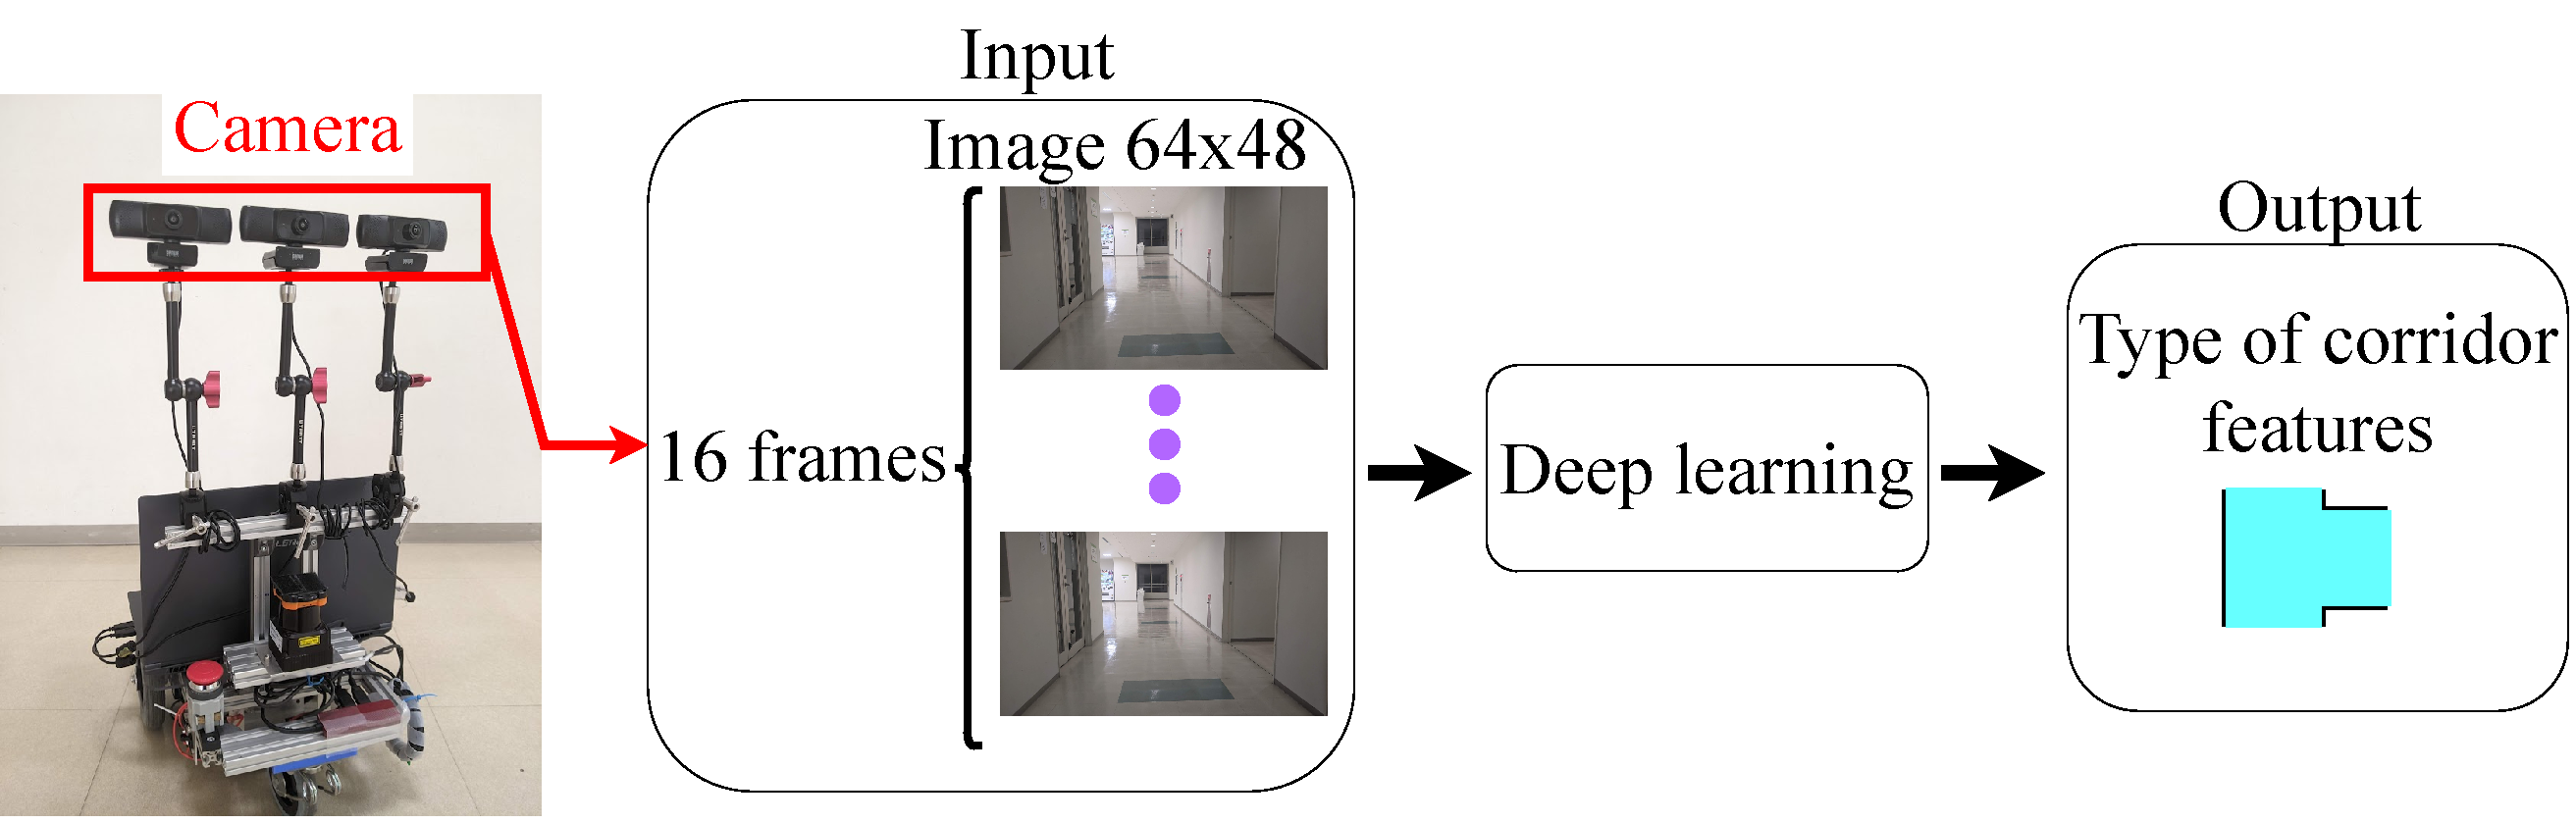
\includegraphics[width=100mm]{images/pdf/intersection_abs.pdf}
     \caption[Overview of the corridor classification module]{Overview of the corridor classification module(Quoted from \cite{haruyama2023})}
     \label{fig:intersection_abs}
\end{figure}
\begin{figure}[htbp]
    \centering
     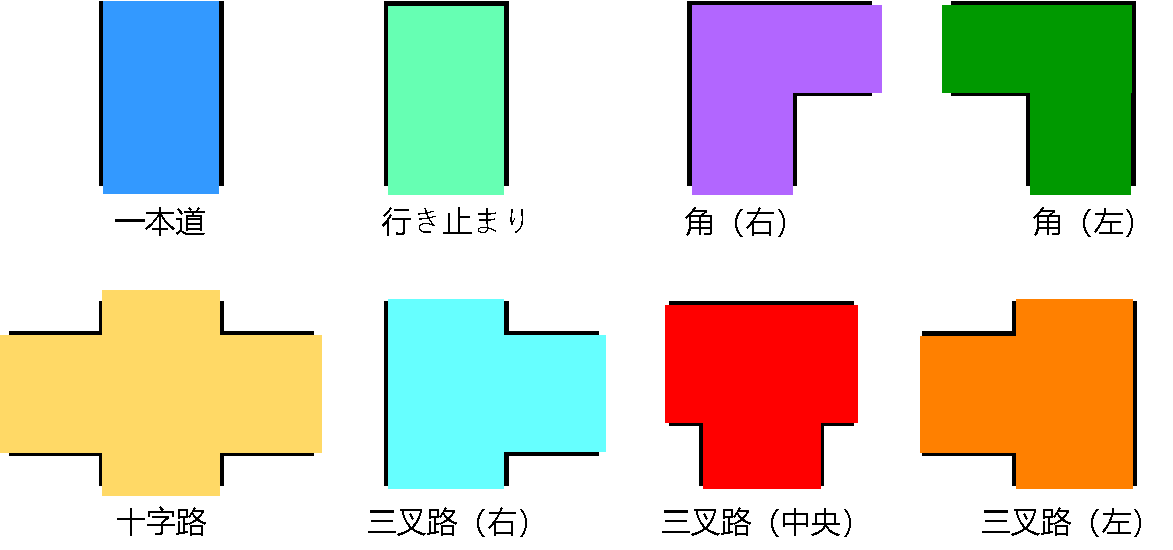
\includegraphics[width=100mm]{images/pdf/class.pdf}
     \caption[Types of corridor features]{Types of corridor features(Quoted from \cite{haruyama2023})}
     \label{fig:class}
\end{figure}
\newpage

ネットワークの構成を\figref{fig:int_net}に示す.
このネットワークアーキテクチャはDhaivatら\cite{lrcn}が提案するCNNとLSTMを組み合わせた
IntersectNetに倣って構築した.
なおCNNアーキテクチャは実時間性の観点からAlexNet\cite{alex}からMobileNetV3-Large\cite{v3}へ変更している.

ネットワークはフレーム数16,画像サイズ64x48の連続したRGB画像データを入力とする.
画像データは各フレームごとにCNNで処理され,この特徴ベクトルはLSTMへ入力される.
各LSTMの出力は分類層(全結合層)へ渡される.
最後に,すべての分類層の出力を融合層へ渡し,融合層は入力の平均を取ることで,
最終的な分類結果を出力する.
活性化関数としてReLU,最適化アルゴリズムにはAdam,損失関数としてCrossEntropyLossを使用する.
\begin{figure}[htbp]
    \centering
     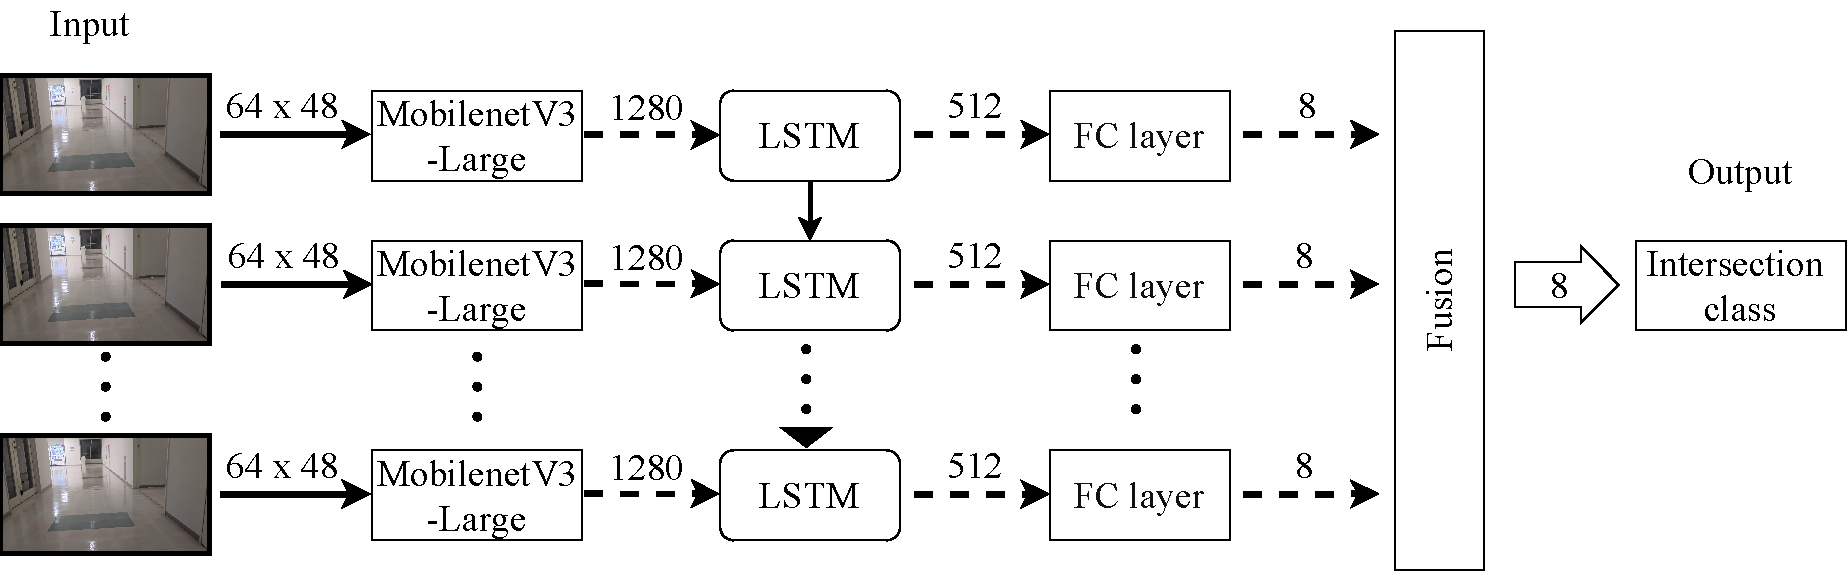
\includegraphics[width=120mm]{images/pdf/network-intersect.pdf}
     \caption{Network of corridor classification module}
     \label{fig:int_net}
\end{figure}

\newpage
次に通路分類モジュールのデータセットの作成について述べる.
データの作成では,経路追従モジュールの学習と同様に,
メトリックマップに基づいたルールベース制御器によって経路を走行する.
その際,フレーム数 16 の連続したカメラ画像と通路の分類ラベルを1組とし,
0.125秒周期でデータセットへ加える.分類ラベルのアノテーションは,
\figref{fig:int_net}に示すように,通路の特徴を予めメトリックマップに登録しておくことで,自動的に行う.
\begin{figure}[htbp]
    \centering
     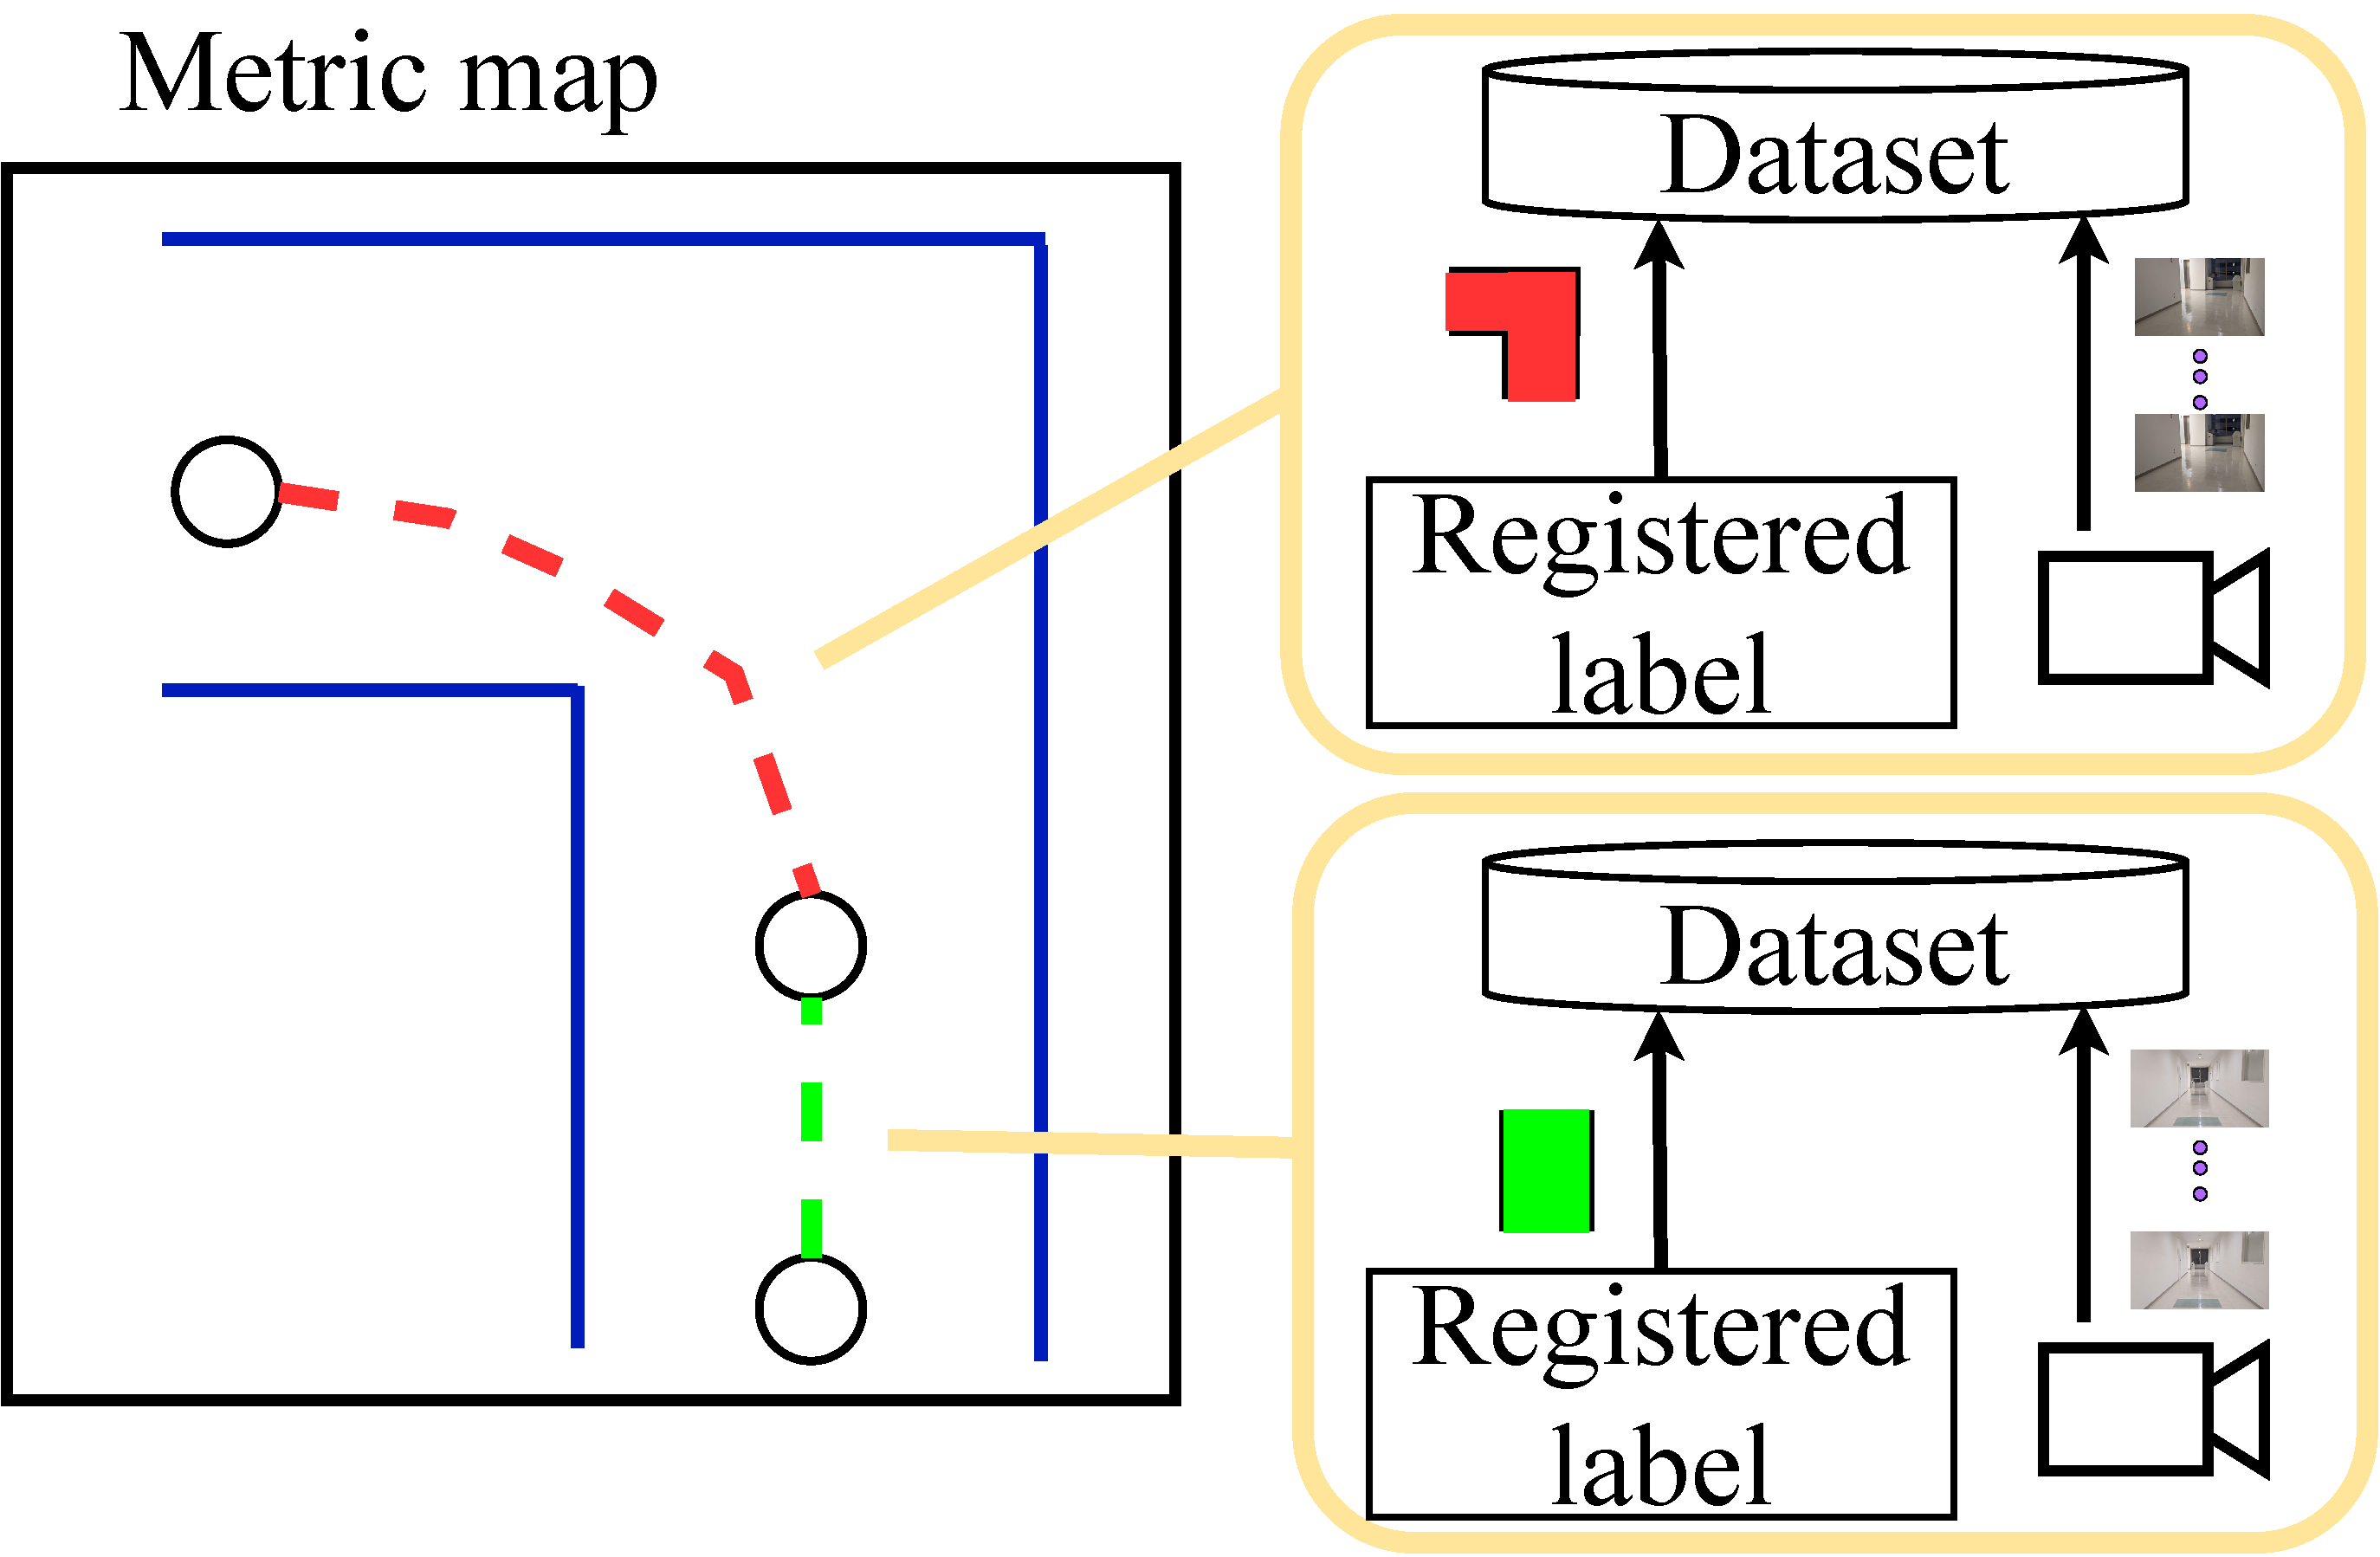
\includegraphics[width=100mm]{images/pdf/map_label.pdf}
     \caption[Classification labels registered in the metric map]{Classification labels registered in the metric map(Quoted from \cite{haruyama2023})}
     \label{fig:int_net}
\end{figure}

\secref{sec:imitation}では不均衡データへの対策として,オーバーサンプリングを行った.
この通路文類モジュールでは,不均衡データへの対策として,
データセット内のクラス間のデータ数によって重み付けを行うコストアプローチ\cite{cost}を行う.
具体的には,損失関数(CrossEntropyLoss)で用いるクラスごとの重みをデータ数を基に調整する.
\newpage
\section{シナリオモジュール}
\label{sec:scenario}
シナリオモジュールについて述べる.
シナリオモジュールはトポロジカルマップから作成されたシナリ
オから「突き当りまで」という「条件」や「左折」なとの「行動」を解釈し,
単語で構成された経路を分岐路での目標方向へ変換して出力する.

\figref{fig:topo2sce}にトポロジカルマップとそれをもとに作成されるシナリオを示す.
図の例では出発地点をエッジ2,目的地をノード2として,その間のエッジとノードを移動する.
エッジ2からノード1は「三叉路まで」という条件と「直進」という行動,
ノード1からエッジ1は「右折」という行動,
エッジ1からノード2は「突き当り(三叉路)まで」という条件と「直進」の行動で表現される.
これらを統合すると,
最終的に「三叉路まで直進.右折.突き当たりまで直進.停止.」
のシナリオが作成される.

次に作成したシナリオを目標方向に変換する処理を述べる.
はじめにシナリオを句点ごとに分解し,部分シナリオというものを作成する.
この部分シナリオには,次の部分シナリオに遷移するための「条件」とロボットが行う必要がある「行動」
が含まれている.
この部分シナリオを形態素分析(MeCab\cite{2004ConditionalRF})を用いて単語へ分割する.
分割した単語は,「条件」と「行動」を示す以下の項目に分けて登録される.
\begin{enumerate}
    \item [1)] 通路の特徴 例えば,「三叉路」「角」など
    \item [2)] 順番 例えば,「3 つ目の」「2 番目の」など 
    \item [3)] 方向 例えば,「左手に」「右手に」など
    \item [4)] 行動 例えば,「右折」「停止」など
\end{enumerate}
先に示した例は句点ごとに,
三叉路まで直進/ 
右折/   
突き当たりまで直進/  
停止/ 
と分解される.

1つ目の条件と行動は 
1)通路の特徴 三叉路,4)行動 直進,

2つ目の行動は 4)行動 右折となる.

3つ目の条件と行動は
1)通路の特徴 突き当たり 4)行動 直進

4つ目の行動は
4)停止となる.

この4)行動を\tabref{tab:target}で示したデータ形式で表現し,分岐路での目標方向として,経路追従モジュールへ与える.
ここで,「三叉路まで」といった条件を達成したかの判定は,
\secref{sec:intersection}の通路分類モジュールの分類結果を用いて行う.
\vspace{3zh}
\begin{figure}[htbp]
    \centering
     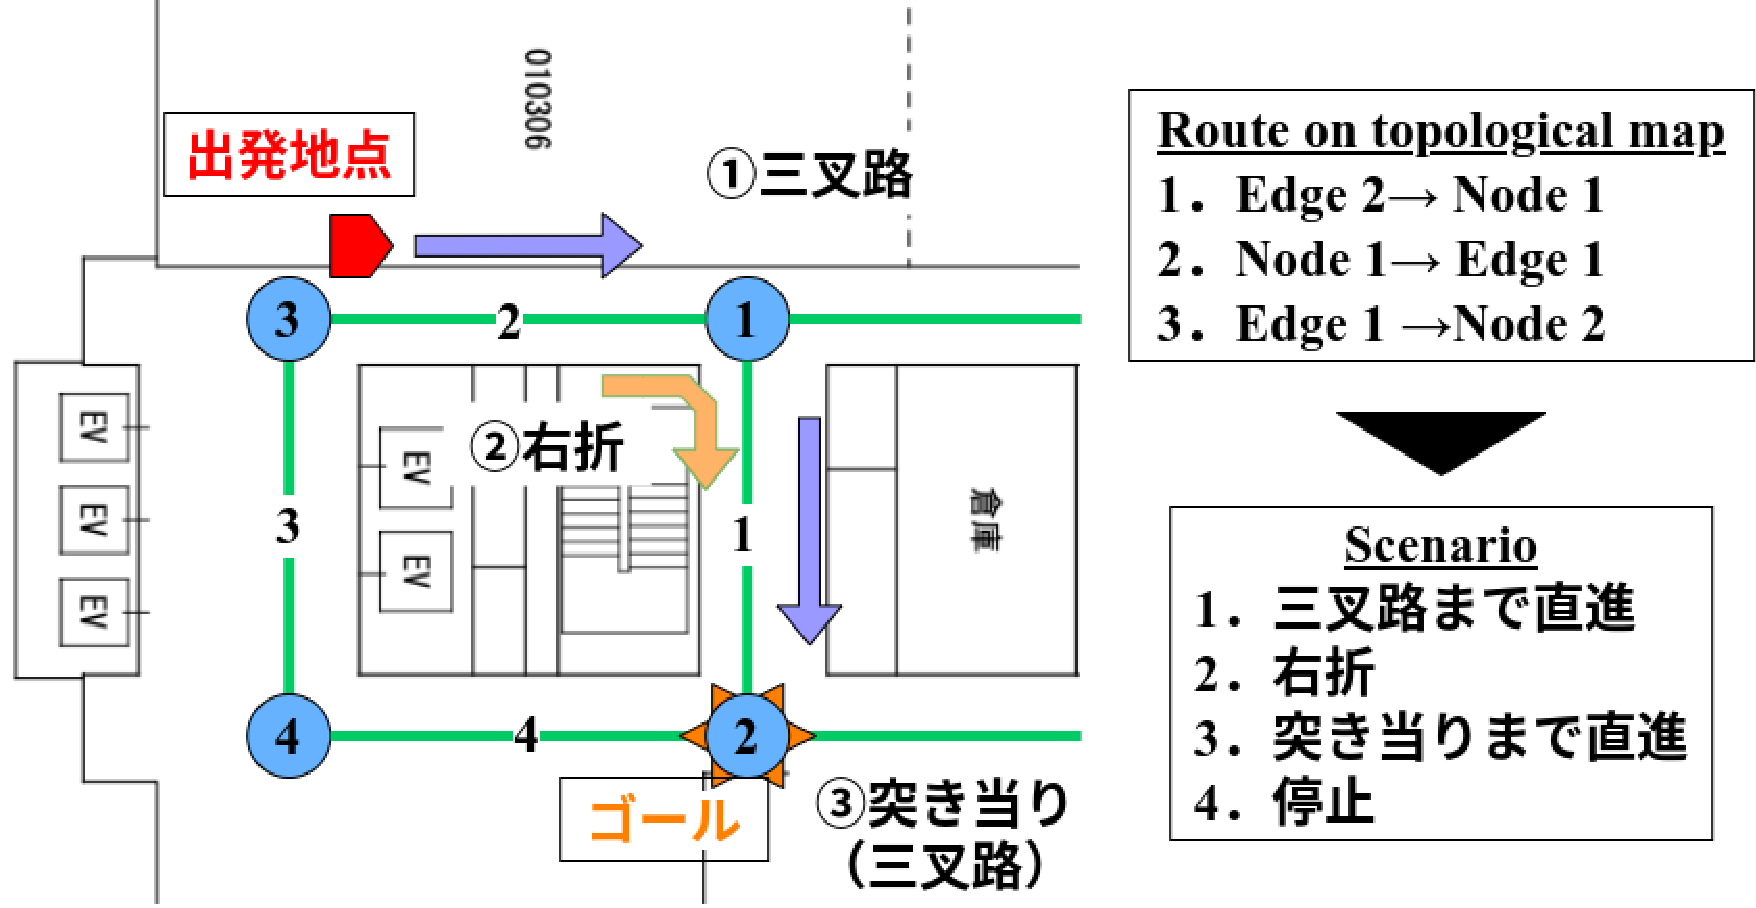
\includegraphics[width=90mm]{images/pdf/topo2sce.pdf}
     \caption[Example of topological map and created scenario]{Example of topological map and created scenario(Quoted from \cite{haruyama2023})}
     \label{fig:topo2sce}
\end{figure}
\newpage
\section{実ロボットを用いた実験}
実ロボットを用いて, 構築したシステムにより, 
ロボットが目的地へ到達可能であるか検証する.
\subsection{実験装置}
実験で用いるロボットを\figref{fig:gamma}に示す.
ロボットはicart-mini\cite{icart}をベースに開発したロボットを用いる.
センサとして,単眼のウェブカメラ(サンワサプライ株式会社 CMS-V43BK)を3つ,
2D-LiDAR(北陽電機 UTM-30LX)を1つ,左右のモータにそれぞれパルス付きエンコーダを搭載している.
制御用の PC には GALLERIA GCR2070RGF-QC-Gを使用している.
メトリックマップに基づくルールベース制御器には,本学でROS Navigation stackをもとに開発した
orne\_navigation\cite{orne_nav}を使用する
\begin{figure}[htbp]
    \centering
     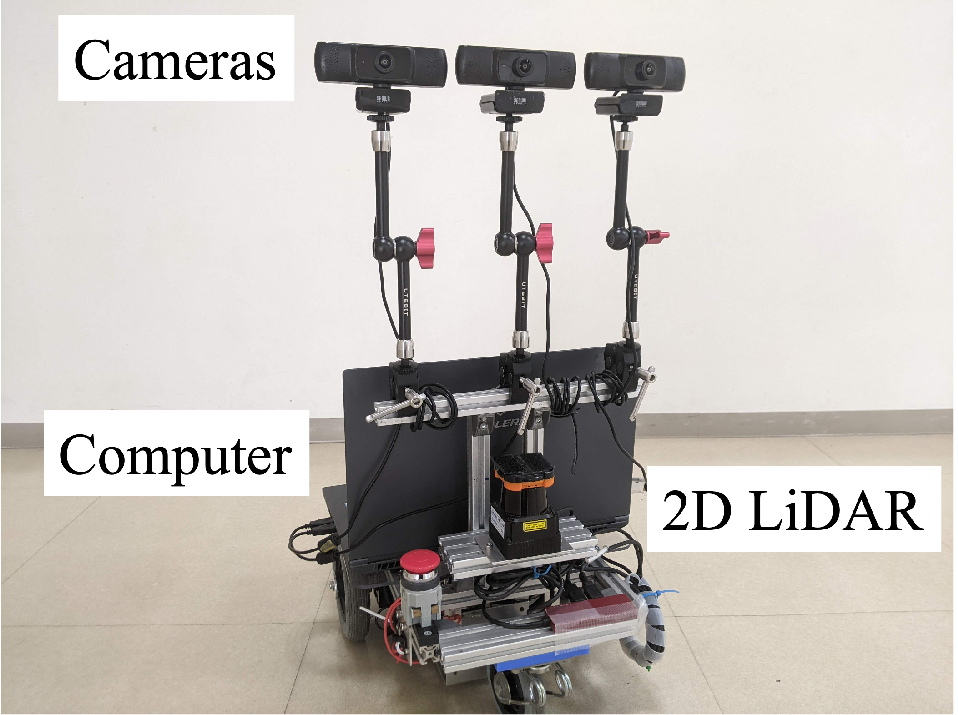
\includegraphics[width=80mm]{images/pdf/gamma_sensor.pdf}
     \caption{Experimental setup (Quoted from \cite{haruyama2023})}\label{fig:gamma}
\end{figure}

\newpage
\subsection{実験方法}
実験環境として\figref{fig:cit3f}に示す千葉工業大学津田沼キャンパス2号館3階の廊下を用いる.
環境中には,三叉路が4つ,角が2つ,突き当たりが2つ含まれている.
経路追従モジュールの訓練および通路分類モジュールのデータセット収集では,
\figref{fig:newroute}で示すaからnの経路を順番に走行する.
\begin{figure}[htbp]
    \centering
     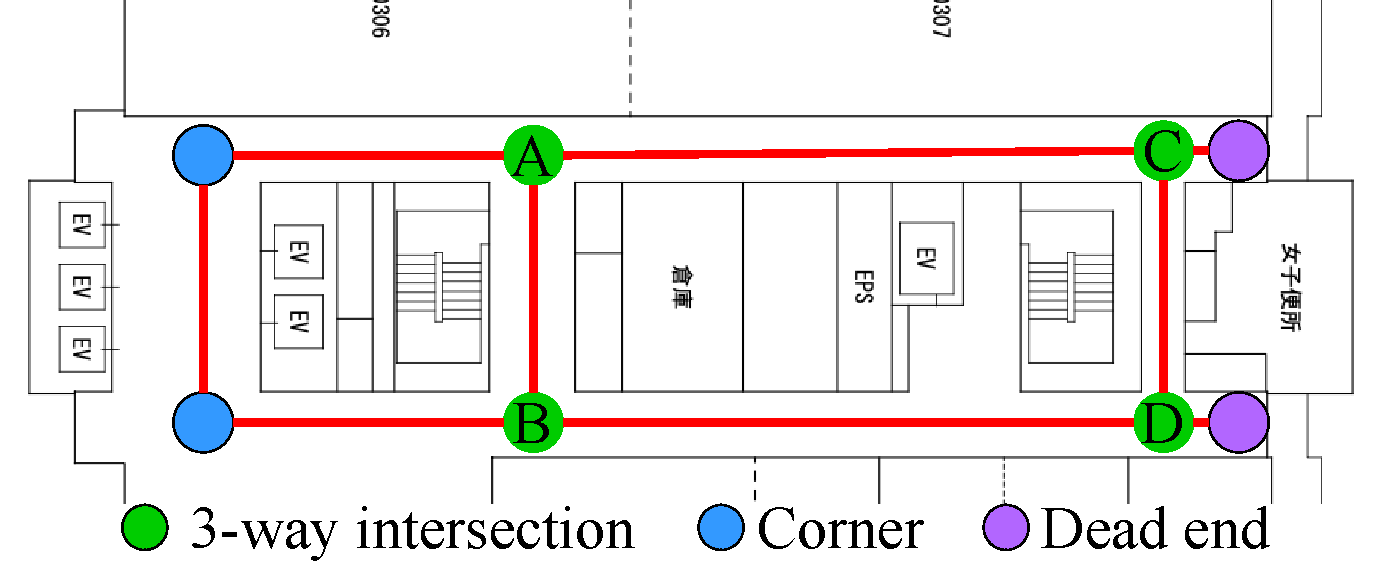
\includegraphics[width=100mm]{images/pdf/cit3f.pdf}
     \caption{Experimental environment (Quoted from \cite{haruyama2023})}\label{fig:cit3f}
\end{figure}
\begin{figure}[htbp]
    \centering
     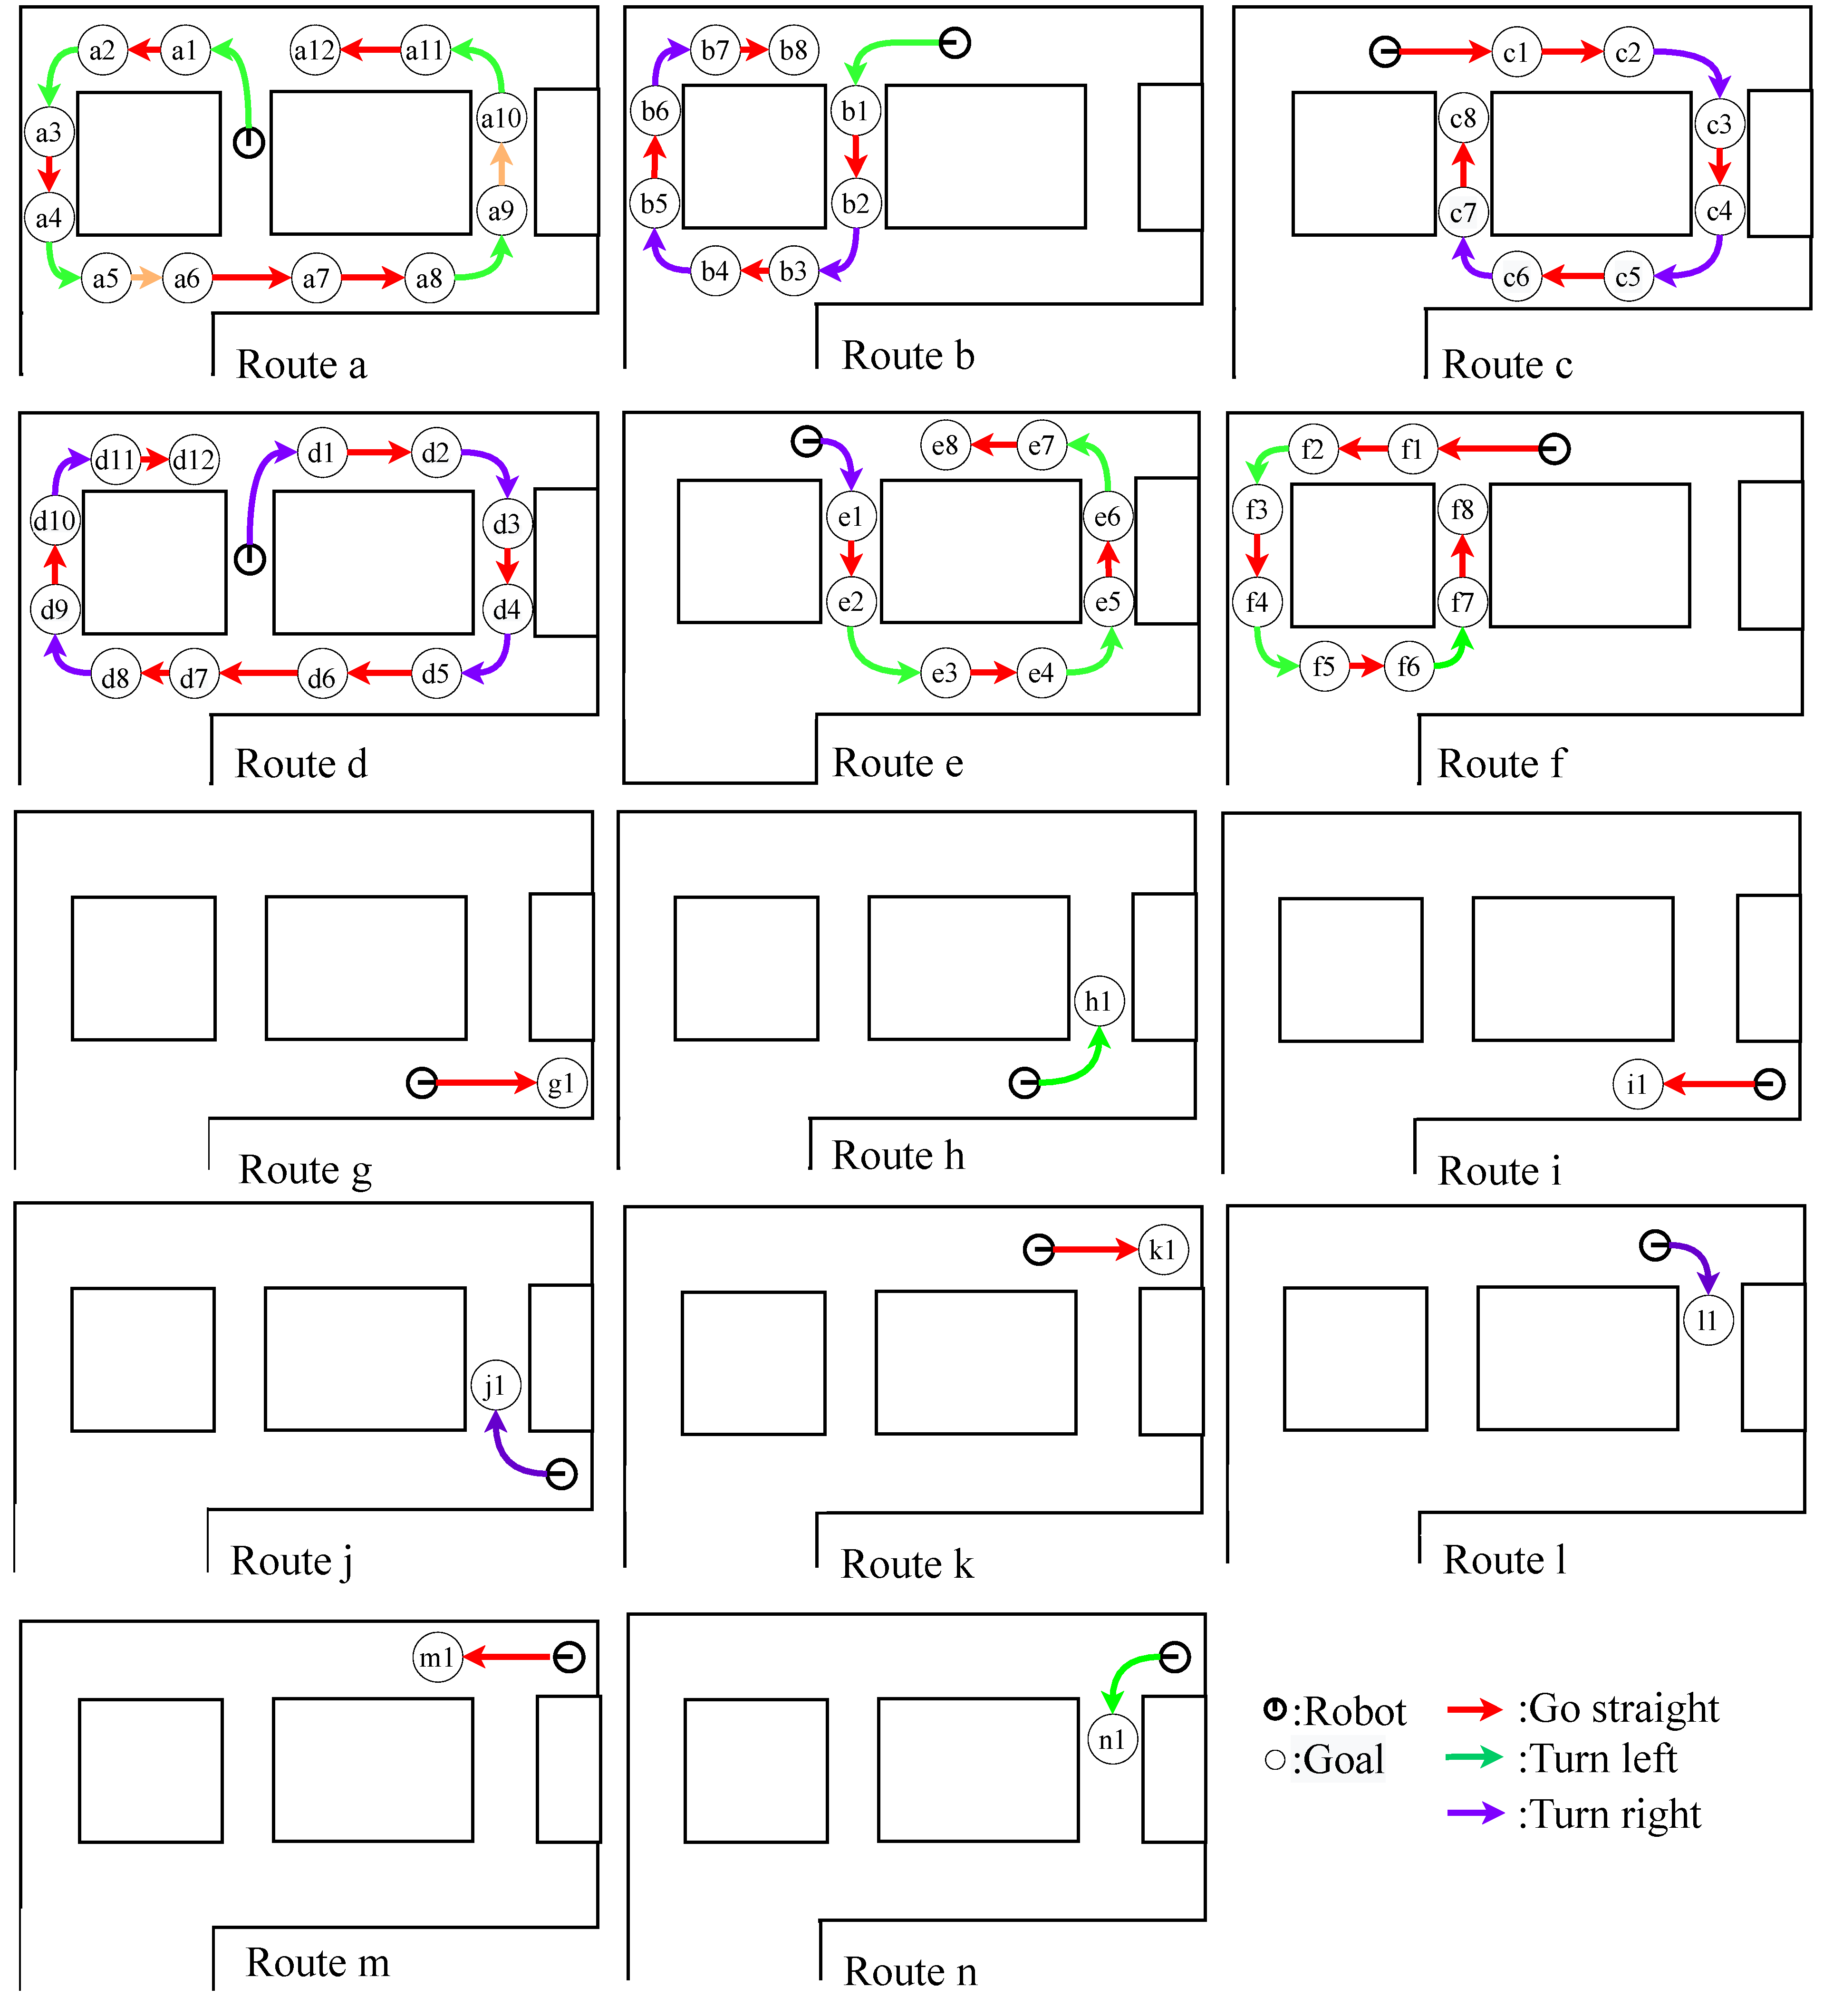
\includegraphics[width=130mm]{images/pdf/si_route.pdf}
     \caption{Route used for learning (Quoted from \cite{haruyama2023})}\label{fig:newroute}
\end{figure}


\subsubsection{シナリオの選定}
実験では島田らが用いた50例のシナリオの中から,
\figref{fig:scenario_exp}に示す7例を用いた.
このシナリオは以下の3つの基準に従って,選定した.
% \ref{fig:cit3f}の場所を対象としていること.
% ロボットが移動困難な\ref{fig:semai}の箇所のような狭い通路が含まれていないこと.
% その場で「後ろを向く」など経路追従モジュールができない行動が含まれていないことである.
\begin{enumerate}
    \item [1)] 2号館3階の廊下において,\figref{fig:cit3f}の場所を対象としていること.
    \item [2)] ロボットが移動困難な\figref{fig:semai}の箇所のような狭い通路が含まれていないこと
    \item [3)] その場で「後ろを向く」など経路追従モジュールができない行動が含まれていないこと
\end{enumerate}

\begin{figure*}[htbp]
    \begin{tabular}{ccc}
        \begin{minipage}[t]{0.5\textwidth}
            \centering
            \includegraphics[keepaspectratio, width=57mm]{images/pdf/scenario/scenario01.pdf}
            \subcaption{Scenario 01}
            \label{composite}
        \end{minipage} &
        \begin{minipage}[t]{0.5\textwidth}
            \centering
            \includegraphics[keepaspectratio, width=57mm]{images/pdf/scenario/scenario02.pdf}
            \subcaption{Scenario 02}
            \label{Gradation}
        \end{minipage} \\
        \begin{minipage}[t]{0.5\textwidth}
            \centering
            \includegraphics[keepaspectratio, width=57mm]{images/pdf/scenario/scenario03.pdf}
            \subcaption{Scenario 03}
            \label{fill}
        \end{minipage} &
        \begin{minipage}[t]{0.5\textwidth}
            \centering
            \includegraphics[keepaspectratio, width=57mm]{images/pdf/scenario/scenario04.pdf}
            \subcaption{Scenario 04}
            \label{fig:scenario21}
        \end{minipage} \\
        \begin{minipage}[t]{0.5\textwidth}
            \centering
            \includegraphics[keepaspectratio, width=57mm]{images/pdf/scenario/scenario05.pdf}
            \subcaption{Scenario 05}
            \label{image1}
        \end{minipage} &
        \begin{minipage}[t]{0.5\textwidth}
            \centering
            \includegraphics[keepaspectratio, width=57mm]{images/pdf/scenario/scenario06.pdf}
            \subcaption{Scenario 06}
            \label{fig:scenario24}
        \end{minipage}\\
        \begin{minipage}[t]{0.5\textwidth}
            \centering
            \includegraphics[keepaspectratio, width=57mm]{images/pdf/scenario/scenario07.pdf}
            \subcaption{Scenario 07}
            \label{imagess}
        \end{minipage}
    \end{tabular}
    \caption{Scenarios used in the experiment (Quoted from \cite{haruyama2023})}\label{fig:scenario_exp}
\end{figure*}

\begin{figure}[htbp]
    \centering
     \includegraphics[width=130mm]{images/pdf/sce_semai.pdf}
     \caption{Example of narrow passage in experimental environment}\label{fig:semai}
\end{figure}

\clearpage
\subsubsection{通路追従モジュールの訓練}
まずはじめに通路分類モジュールの訓練を行う.
前述の経路をメトリックマップに基づいたルールベース制御器の出力を用いて,
3周し,データセットを収集する.
収集したデータは,1,2周目を訓練データとし,
3周目をテストデータとする.それぞれのデータ数は,
訓練データ5781,テストデータ2902であり.2つのデータ内のクラス間のデータ数は\tabref{tab:dataset}である.
訓練は損失関数の重みを\tabref{tab:cost},バッチサイズを32として,30epoch行った.

訓練後,テストデータに対する通路分類モジュールの正解率{(Accuracy)},適合率{(Precision)}を計算する.
\begin{table}[htbp]
    \centering
    \caption{Number of classes in the dataset}\label{tab:dataset}
    \begin{tabular}{c|c|c}
    \hline
    Class & Learning data &Test data        \\
    \hline
    直進   & 2760 & 1377\\
    突き当たり   & 90 & 45 \\
    角(右) & 549 & 279 \\
    角(左)& 567 & 288 \\
    十字路 & 0 & 0 \\
    三叉路(右)& 753 & 387 \\
    三叉路(中央)& 306 & 153 \\
    三叉路(左) & 747 & 369 \\
    \hline
    \end{tabular}
\end{table}

\begin{table}[htbp]
    \centering
    \caption{The weights assigned to each class in the experiment}\label{tab:cost}
    \begin{tabular}{c|c}
    \hline
    Class & Class weights         \\
    \hline
    直進   & 1\\
    突き当たり   & 5\\
    角(右) & 5\\
    角(左)& 5 \\
    十字路 & 1  \\
    三叉路(右)& 5  \\
    三叉路(中央)& 10  \\
    三叉路(左) & 5  \\
    \hline
    \end{tabular}
\end{table}
\subsubsection{経路追従モジュールの訓練}
次に経路追従モジュールの訓練を行う.
通路分類モジュールの訓練と同様の経路を,
オンラインで 模倣学習しながら1周走行する.
その際のステップ数は12000であった.

2つのモジュールを訓練後,シナリオを1例ずつ入力して,
ロボットの挙動を観察する.実験では,ロボットをシナリオの
スタート地点に移動して,自律移動を開始する.

\vspace{5zh}



\newpage
\subsection{実験結果}
テストデータに対する,通路分類モジュールの正解率と適合率を\tabref{tab:result}に示す.
この計算にはモデル評価用ライブラリである
torcheval\cite{torcheval}を用いた.
\begin{table}[htbp]
    \centering
    \caption{Evaluation results of the corridor classification module on test data.}
    \label{tab:result}
    \begin{tabular}{c|c}
    \hline
    Metrics & Value       \\
    \hline
    Accuracy   & 0.98 \\
    Precision   & 0.98 \\
    \hline
    \end{tabular}
\end{table}
% \begin{table}[]
%     \centering
%     \caption{intersection あーだのコーダの}\label{tab:acc}
%     \begin{tabular}{|c|c|}
%     \hline
%     指標 & 値
%     \hline
%     accuraty & 0.98 \\
%     適合率 & 0.4 \\
%     \hline
%     \end{tabular}
% \end{table}
% \newpage

\figref{fig:exp_path}に\figref{fig:scenario21}のシナリオを入力した実験の様子を示す.
キャプションは実行中の部分シナリオと,ロボットが現在位置する通路の特徴である.
図に示すように入力されたシナリオの道順に従い, 三叉路などの分岐路
で適切に経路を選択して自律移動する様子が見られた.
結果として,7例すべてでロボットが, 目的地へ到達した.
以上の結果から, 構築したカメラ画像とシナリオに基づいて, 
経路を追従して目的地まで自律移動するシステムの有効性が確認された.

\begin{figure*}[htbp]
    \begin{tabular}{ccc}
        \begin{minipage}[t]{0.5\textwidth}
            \centering
            \includegraphics[keepaspectratio, width=70mm]{images/exp_path_follow_0.png}
            \subcaption{3つ目の三叉路まで直進(First 3-way)}
        \end{minipage} &
        \begin{minipage}[t]{0.5\textwidth}
            \centering
            \includegraphics[keepaspectratio, width=70mm]{images/exp_path_follow_1.png}
            \subcaption{3つ目の三叉路まで直進(Second 3-way)}
        \end{minipage} \\

        \begin{minipage}[t]{0.5\textwidth}
            \centering
            \includegraphics[keepaspectratio, width=70mm]{images/exp_path_follow_2.png}
            \subcaption{右折(Third 3-way)}
        \end{minipage} &
        \begin{minipage}[t]{0.5\textwidth}
            \centering
            \includegraphics[keepaspectratio, width=70mm]{images/exp_path_follow_4.png}
            \subcaption{突き当たりまで直進(Straight road)}
        \end{minipage} \\
        \begin{minipage}[t]{0.5\textwidth}
            \centering
            \includegraphics[keepaspectratio, width=70mm]{images/exp_path_follow_5.png}
            \subcaption{左折(End)}
        \end{minipage} &
        \begin{minipage}[t]{0.5\textwidth}
            \centering
            \includegraphics[keepaspectratio, width=70mm]{images/exp_path_follow_6.png}
            \subcaption{突き当たりまで直進(Straight road)}
        \end{minipage} \\
        \begin{minipage}[t]{0.5\textwidth}
            \centering
            \includegraphics[keepaspectratio, width=70mm]{images/exp_path_follow_7.png}
            \subcaption{停止(End)}
        \end{minipage}
    \end{tabular}

    \caption{An example of the robot applied the constructed system (Quoted from \cite{haruyama2023})}\label{fig:exp_path}
\end{figure*}
% \chapter{実ロボットを用いた実験}
\label{chap:experiment}
%
%\input{introduction/preface}
%
% \section{通路分類モジュールの}
\section{実験概要}
実ロボットを用いて, 提案するシステムにより, 
ロボットが目的地へ到達可能であるか検証する.
\subsection{実験装置}
実験で用いるロボットを\ref{fig:gamma}に示す.
ロボットはicart-mini\cite{icart}をベースに本研究室で開発した
orne\_gammaを用いる.
センサとして,単眼のウェブカメラ(サンワサプライ株式会社 CMS-V43BK)を3つ,
2D-LiDAR(北陽電機 UTM-30LX)を1つ搭載している. 
また左右のモータにそれぞれパルス付きエンコーダが付属している.
制御用の PC には GALLERIA GCR2070RGF-QC-Gを使用している.
メトリックマップに基づくナビゲーションには,本学でNavigation stackをもとに開発した
orne\_navigation\cite{orne_nav}を使用する
\begin{figure}[htbp]
    \centering
     \includegraphics[width=80mm]{images/pdf/gamma_sensor.pdf}
     \caption{Experimental setup}\label{fig:gamma}
\end{figure}

\newpage
\subsection{実験方法}
実験環境として\ref{fig:cit3f}に示す千葉工業大学津田沼キャンパス2号館3階の廊下を用いる.
環境中には,三叉路が4つ,角が2つ,突き当たりが2つ含まれている.
経路追従モジュールの訓練および通路分類モジュールのデータセット収集では,
\ref{fig:newroute}で示したaからnの経路を順番に走行する.
\begin{figure}[htbp]
    \centering
     \includegraphics[width=100mm]{images/pdf/cit3f.pdf}
     \caption{Experimental environment \cite{haruyama2023}}\label{fig:cit3f}
\end{figure}
\begin{figure}[htbp]
    \centering
     \includegraphics[width=130mm]{images/pdf/newroute.pdf}
     \caption{Experimental environment Quoted from \cite{haruyama2023}}\label{fig:newroute}
\end{figure}


\subsubsection{シナリオの選定}
実験では島田らが用いた50例のシナリオの中から,
〜に示す7例を用いた.
このシナリオは以下の3つの基準に従って,選定した.
% \ref{fig:cit3f}の場所を対象としていること.
% ロボットが移動困難な\ref{fig:semai}の箇所のような狭い通路が含まれていないこと.
% その場で「後ろを向く」など経路追従モジュールができない行動が含まれていないことである.
\begin{enumerate}
    \item [1)] \ref{fig:cit3f}の場所を対象としていること.
    \item [2)] ロボットが移動困難な\ref{fig:semai}の箇所のような狭い通路が含まれていないこと
    \item [3)] その場で「後ろを向く」など経路追従モジュールができない行動が含まれていないこと
\end{enumerate}

\begin{figure*}[htbp]
    \begin{tabular}{ccc}
        \begin{minipage}[t]{0.5\textwidth}
            \centering
            \includegraphics[keepaspectratio, width=57mm]{images/pdf/scenario/scenario01.pdf}
            \subcaption{Scenario 01}
            \label{composite}
        \end{minipage} &
        \begin{minipage}[t]{0.5\textwidth}
            \centering
            \includegraphics[keepaspectratio, width=57mm]{images/pdf/scenario/scenario02.pdf}
            \subcaption{Scenario 02}
            \label{Gradation}
        \end{minipage} \\
        \begin{minipage}[t]{0.5\textwidth}
            \centering
            \includegraphics[keepaspectratio, width=57mm]{images/pdf/scenario/scenario03.pdf}
            \subcaption{Scenario 03}
            \label{fill}
        \end{minipage} &
        \begin{minipage}[t]{0.5\textwidth}
            \centering
            \includegraphics[keepaspectratio, width=57mm]{images/pdf/scenario/scenario04.pdf}
            \subcaption{Scenario 04}
            \label{transform}
        \end{minipage} \\
        \begin{minipage}[t]{0.5\textwidth}
            \centering
            \includegraphics[keepaspectratio, width=57mm]{images/pdf/scenario/scenario05.pdf}
            \subcaption{Scenario 05}
            \label{image1}
        \end{minipage} &
        \begin{minipage}[t]{0.5\textwidth}
            \centering
            \includegraphics[keepaspectratio, width=57mm]{images/pdf/scenario/scenario06.pdf}
            \subcaption{Scenario 06}
            \label{fig:scenario24}
        \end{minipage}\\
        \begin{minipage}[t]{0.5\textwidth}
            \centering
            \includegraphics[keepaspectratio, width=57mm]{images/pdf/scenario/scenario07.pdf}
            \subcaption{Scenario 07}
            \label{imagess}
        \end{minipage}
    \end{tabular}
    \caption{Scenarios used in the experiment Quoted from \cite{haruyama2023}}\label{fig:scenario_exp}
\end{figure*}

\begin{figure}[htbp]
    \centering
     \includegraphics[width=100mm]{images/pdf/sce_semai.pdf}
     \caption{Experimental environment}\label{fig:semai}
\end{figure}

\newpage
\subsubsection{通路追従モジュールの訓練}
まずはじめに通路分類モジュールの訓練を行う.
前述の経路をメトリックマップに基づいたルールベース制御器の出力を用いて,
3周し,データセットを収集する.
収集したデータは,1,2 周目を訓練データとし,
3周目をテストデータとする.それぞれのデータ数は,
訓練データ 5781,テストデータ 2902 である. 
この訓練データ内のクラス間のデータ数は〜であり,訓練は
損失関数の重みを〜,バッチサイズを32として,30epoch行った.

訓練後,テストデータに対する通路分類モジュールの正解率{(Accuracy)},適合率{(Precision)}を計算する.
\begin{table}[htbp]
    \centering
    \caption{Number of classes in the dataset}\label{tab:target}
    \begin{tabular}{c|c|c}
    \hline
    Class & Learning data &Test data        \\
    \hline
    直進   & 2760 & 1377\\
    突き当たり   & 90 & 45 \\
    角(右) & 549 & 279 \\
    角(左)& 567 & 288 \\
    十字路 & 0 & 0 \\
    三叉路(右)& 753 & 387 \\
    三叉路(中央)& 306 & 153 \\
    三叉路(左) & 747 & 369 \\
    \hline
    \end{tabular}
\end{table}

\begin{table}[htbp]
    \centering
    \caption{cost}\label{tab:cost}
    \begin{tabular}{c|c}
    \hline
    Class & Class weights         \\
    \hline
    直進   & 1\\
    突き当たり   & 5\\
    角(右) & 5\\
    角(左)& 5 \\
    十字路 & 1  \\
    三叉路(右)& 5  \\
    三叉路(中央)& 10  \\
    三叉路(左) & 5  \\
    \hline
    \end{tabular}
\end{table}
\subsubsection{経路追従モジュールの訓練}
次に経路追従モジュールの訓練を行う.
通路分類モジュールの訓練と同様の経路を,
オンラインで 模倣学習しながら1周走行する.
その際のステップ数 は 12000 であった.

2つのモジュールを訓練後,シナリオを1例ずつ入力して,
ロボットの挙動を観察する.実験では,ロボットをシナリオの
スタート地点に移動して,自律移動を開始する.

\vspace{5zh}



\newpage
\subsection{実験結果}
テストデータに対する,通路分類モジュールの正解率と適合率を\ref{tab:result}に示す.
この計算にはpytorchのモデル評価用ライブラリである
torcheval\cite{torcheval}を用いて算出する.
\begin{table}[htbp]
    \centering
    \caption{Target direction and data for path-following module}
    \label{tab:result}
    \begin{tabular}{c|c}
    \hline
    指標 & 値        \\
    \hline
    Accuracy   & 0.98 \\
    Precision   & 0.4 \\
    \hline
    \end{tabular}
\end{table}
% \begin{table}[]
%     \centering
%     \caption{intersection あーだのコーダの}\label{tab:acc}
%     \begin{tabular}{|c|c|}
%     \hline
%     指標 & 値
%     \hline
%     accuraty & 0.98 \\
%     適合率 & 0.4 \\
%     \hline
%     \end{tabular}
% \end{table}
% \newpage

\ref{fig:exp_path}に\ref{fig:scenario_exp}のシナリオを入力した実験の様子を示す.
図に示すように入力されたシナリオの道順に従い, 三叉路などの分岐路
で適切に経路を選択して自律移動する様子が見られた.
結果として,7例すべてでロボットが, 目的地へ到達した.
以上の結果から, 提案するカメラ画像とシナリオに基づいて, 
経路を追従して目的地まで自律移動するシステムの有効性が確認された.

\begin{figure*}[htbp]
    \begin{tabular}{ccc}
        \begin{minipage}[t]{0.5\textwidth}
            \centering
            \includegraphics[keepaspectratio, width=70mm]{images/exp_path_follow_0.png}
            \subcaption{3つ目の三叉路まで直進(First 3-way)}
        \end{minipage} &
        \begin{minipage}[t]{0.5\textwidth}
            \centering
            \includegraphics[keepaspectratio, width=70mm]{images/exp_path_follow_1.png}
            \subcaption{3つ目の三叉路まで直進(Second 3-way)}
        \end{minipage} \\

        \begin{minipage}[t]{0.5\textwidth}
            \centering
            \includegraphics[keepaspectratio, width=70mm]{images/exp_path_follow_2.png}
            \subcaption{右折(Third 3-way)}
        \end{minipage} &
        \begin{minipage}[t]{0.5\textwidth}
            \centering
            \includegraphics[keepaspectratio, width=70mm]{images/exp_path_follow_4.png}
            \subcaption{突き当たりまで直進(Straight road)}
        \end{minipage} \\
        \begin{minipage}[t]{0.5\textwidth}
            \centering
            \includegraphics[keepaspectratio, width=70mm]{images/exp_path_follow_5.png}
            \subcaption{左折(End)}
        \end{minipage} &
        \begin{minipage}[t]{0.5\textwidth}
            \centering
            \includegraphics[keepaspectratio, width=70mm]{images/exp_path_follow_6.png}
            \subcaption{突き当たりまで直進(Straight road)}
        \end{minipage} \\
        \begin{minipage}[t]{0.5\textwidth}
            \centering
            \includegraphics[keepaspectratio, width=70mm]{images/exp_path_follow_7.png}
            \subcaption{停止(End)}
        \end{minipage}
    \end{tabular}

    \caption{An example of the robot applied the proposed system Quoted from \cite{haruyama2023}}\label{fig:exp_path}
\end{figure*}
%

\chapter{おわりに}
\label{chap:end}
\section{結論}
本論文では,
岡田らの従来手法に対し,動的に経路を選択して走行する機能や
視覚に基づいて通路の特徴を検出する機能,分岐路において目的地に向けた進行方向を提示する機能を追加することで,
走行する経路を一定の経路から,設定した任意の目的地に向けた経路へ拡張した.

はじめに経路選択機能の追加を目的として,データセットと学習器の入力へ目標方向を加えた.
そして,追加した機能の有効性をシミュレータを用いた実験により検証した.
実験では,視覚に基づくナビゲーションにおいて,
同一の分岐路であっても目標方向の入力に従い, 
ロボットが適切に経路を選択して移動する様子が見られた.

次に,視覚から通路の特徴を検出する機能,分岐路で目標方向を提示する機能を追加した.
目標方向を提示する機能には,島田らが提案したトポロジカルマップと
「条件」や「行動」による経路の表現(シナリオ)を用いた.
これにより,視覚に基づいて任意の目的地まで移動するシステムを構築した.
そして,実ロボットを用いた実験を行い,構築したシステムにより,カメラ画像とシナリオに基づいて, 
経路を追従し,ロボットが目的地へ到達できることを確認した.

% 事前に作成したメトリックマップを用いず, 
% カメラ画像とシナリオに基づいて経路を追従して目的地まで
% 自律移動するシステムを提案した.
% そして, 実ロボットを用いた実験により提案システムの有効性を検証した.
% 実験では, 提案システムにより,ロボットが目的地へ到達可能であることを
% 確認した.
% \section{今後の展望}
% 本論文では,津田沼キャンパス2号館3階の一部の廊下を対象として実験を行った.
% 今後の展望として,2号館3階のすべての廊下や屋外環境での実験が考えられる.
%% Back Matter
\backmatter{}
%
%!TEX root = ../thesis.tex
% \bibliographystyle{junsrt}
% \bibliography{main_bibliography}
% \usepackage[backend=biber,style=numeric, sorting=none]{biblatex} % biblatexを使用するためのパッケージ
% \addbibresource{main_bibliography.bib}
%
% \input{backmatter/appendix}
%
%!TEX root = ../thesis.tex
\chapter*{謝辞}
\addcontentsline{toc}{chapter}{謝辞}

本研究を進めるにあたり,熱心にご指導を頂いた林原靖男教授と上田隆一准教授に深く感謝いたします.
屋外自律移動ミーティングや研究相談で厳しくご指導いただきました.
これにより,研究や技術的,人間的に成長できました.
また,ご指導のおかげで2回の学会発表を行うことができました.
(この修論の有様のように,文章を書く力は疑問が残りますが)

つくばチャレンジを通して実世界でロボットを動かす経験を積むことができました.
この活動を通して,目的に必要な技術をリサーチし,それに基づいて実装する力と,挑戦を恐れず「手を動かして考える」
といった物事に取り組む姿勢を得ることができました.
また,学部3年で配属されてからの,計4年もの間,研究室で活動しました.
その中で,LiDARとIMUを信じられない破壊をしたことについて大変申し訳なく思っています.

研究面での議論やサポート,私生活などで
岡田眞也先輩,清岡優祐先輩には返しきれぬおんがあります.

また,研究室の同期,後輩(特に屋外自律三人衆)には日々の生活の中で,
研究に関する議論や,息抜きをしていただたことに感謝します.
そして,学部生の頃より.精神的に辛い時の支えと生活に潤いをくださった彼女へ
感謝いたします.
最後に,大学院を卒業するまでの24年間,私を育てていただいた両親に謝意を表します.



%

\end{document}